\chapter{Design of an FPGA-based LEKID spectrometer}\label{readout}

The ASU open-source LEKID readout is a 1,000-channel transceiver, consisting of digital and analog electronics, firmware and software. This technology builds on the legacy of previous MKID demonstrator instruments which have used Field Programmable Gate Array (FGPA) platforms (e.g. MUSIC \citep{golwala2012status}, ARCONS \citep{mchugh2012readout}, NIKA \citep{monfardini2014latest}, MUSTANG-2 \citep{dicker2014mustang2}, MAKO \citep{swenson2012mako}, SPACEKIDS \citep{van2016multiplexed}, DARKNESS \citep{strader2016digitial}). FPGAs enable the high speed digital signal processing (DSP) techniques which are required for both time and frequency-domain-multiplexed readout (FDM) of superconducting detectors.

The FPGA board which serves as the foundation for the LEKID readout described in this work is the second generation Reconfigurable Open Architecture Computing Hardware (ROACH2), an open-source DSP board developed by the Collaboration for Astronomical Signal Processing and Electronics Research (\citet{werthimer2011casper, hickish2016decade}). The ROACH2 is a general purpose DSP board whose primary use is as a digital backend for radio astronomy observatories. The ASU LEKID readout, which is the subject of this chapter, is one of several MKID readouts which have used the ROACH1/ROACH2 platform, including MUSIC (ROACH1), MAKO (ROACH2), ARCONS (ROACH1/2) and DARKNESS (ROACH2/DARKNESS board).

The design and creation of the readout system was driven by a philosophy based on adaptability and scalability. Consequently, the system now serves as a core part of several current and upcoming astronomical instruments. Among these are balloon-borne (e.g., OLIMPO \citep{masi2019kinetic}, BLAST-TNG \citep{gordon2016}) and ground-based cameras (e.g., TolTEC \citep{austermann2018millimeter}, SuperSpec \citep{wheeler2018superspec}, MUSCAT \citep{brien2018muscat}).

In the following sections, we describe the design and verification of the LEKID readout system, with a primary focus on the system which has been developed for the BLAST-TNG stratospheric balloon platform. The chapter is organized as follows:

\begin{itemize}[nosep]
  \item Section~\ref{sys overview} provides a brief overview of the principal readout functions.
  \item Section~\ref{sys reqs} describes the primary system requirements.
  \item Section~\ref{firmware} details the design and verification of the ROACH2 firmware and DSP algorithms.
  \item Section~\ref{hardware and elec} describes the design and construction of the BLAST-TNG readout hardware and electronics.
  \item Section~\ref{noise verify} presents the results of noise verification measurements.
\end{itemize}

\section{System Requirements}\label{sys reqs}

The core system requirements for a KID readout system fall under categories of multiplexing factor, data rate, noise performance, size, weight, power and cost (SWaP-C) and timing synchronization. The readout system must be able to read out the required number of LEKID detectors at a rate determined by the telescope scan speed while contributing less noise than the detectors and cryogenic low-noise amplifiers (LNAs). To facilitate map mapping, the detector data packets must be timestamped in such a way that makes it possible to later align them with the timing information provided by the pointing system.

It is important to note that the requirements which are discussed here pertain primarily to sub-mm/FIR/mm-wave KID cameras. O/NIR systems have slightly different requirements (see Section~\ref{onir_systems}). The following sections discuss the motivation behind each system requirement. The requirements are listed in Table~\ref{tab:sys reqs}. We begin with an overview of the system.

\begin{table}[!htbp]
\centering
\begin{tabular}{@{}ll@{}}
\dtoprule{}
Parameter & Requirement \\ \midrule
RF bandwidth (MHz) & 512 \\
\gls{Sphase} / chan (dBc/Hz) & $\lesssim$ -95 \\
1/f corner \gls{fc} (Hz) & $\lesssim$ 0.5 \\
Data rate (Hz) & 200--500 \\
Power dissipation (W) & $\lesssim$ 60 \\
Time stamp precision (ms) & $\lesssim$ 1 \\
DAC Tone Resolution (Hz) & $\leq$ 1000 \\
Multiplexing Factor & $\gtrsim$ 500 \\ \dbottomrule{}
\\
\end{tabular}
\caption{LEKID readout system requirements.}
\label{tab:sys reqs}
\end{table}

\subsection{System Overview}\label{sys overview}

The LEKID readout processes 512~MHz of instantaneous complex baseband and RF (radio frequency) bandwidth using quadrature ($I/Q$) signal processing. The total bandwidth is divided between 1,000 channels, each with readout bandwidth of $\sim$30--500~Hz. For each channel, the system outputs a 64-bit $I/Q$ sample at a configurable data rate of $\sim$60--1,000~Hz. The $I/Q$ pairs represent the total transmission of each resonator ($I + jQ = V_{\mathrm{in}}\gls{S21}$), and contain the AM (amplitude modulation) and PM (phase modulation) of the detectors. If the detectors are properly biased, the PM is proportional to the absorbed optical power. For KID readout, typically only the PM is used.

In order to accurately probe the resonant frequency of each detector, the probe (carrier) tones synthesized by the DAC must have a frequency resolution $f_{\mathrm{res}} \lesssim 1,000$~Hz (this requirement scales with the resonator quality factor \gls{Qr}).


To readout the detectors, the system must do the following:

\begin{enumerate}[nosep]
  \item Synthesize a baseband probe tone ($I_{\mathrm{DAC}} + jQ_{\mathrm{DAC}}$) in software and firmware with a unique amplitude, frequency and phase for each resonator.
  \item Generate the tone comb with the digital-to-analog converters (DACs).
  \item Upconvert the tone comb to the RF band of the detectors and send to the detector arrays.
  \item Receive the detector-modulated tone comb.
  \item Downconvert the modulated tone comb from RF to baseband, amplify/attenuate/filter as needed.
  \item Digitize the tone comb and analyze with a polyphase filterbank/Fourier transform (PFB-FFT, see Section~\ref{pfb}).
  \item Discard unwanted FFT bins (remaining bins are labeled as channels).
  \item Digitally demodulate each channel (digital downconverter, see Section~\ref{ddc}).
  \item Optionally apply a finite impulse response filter (FIR) to the demodulated signals.
  \item Coherently accumulate each demodulated signal to filter and downsample to the desired output rate (see Section~\ref{accum}).
  \item Packetize $I$ and $Q$ for each channel into UDP frames, add timing and checksum information.
  \item Stream packets to the data network.
  \item In software, perform all necessary steps to calculate the FM of each resonator, and convert to absorbed optical power.
\end{enumerate}

\vspace{5mm}

\subsection{White Noise}\label{white noise}

The readout noise is characterized by its power spectral density (PSD), \gls{Sxx} $\left[\mathrm{x}^{2}/\mathrm{Hz}\right]$, which consists of additive white Gaussian noise (AWGN, hereafter WN) and 1/f (`one over f') components. The latter is hereafter referred to as flicker noise (FN). The 1/f knee, or corner-frequency \gls{fc} of the FN sets the lower limit on the telescope scan speed $\omega_{\mathrm{scan}}$ and readout rate $f_{\mathrm{ro}}$ which will permit for adequate mapping of the science targets.

\begin{table}[!htbp]
\centering
\begin{tabular}{@{}lccc@{}}
\dtoprule{}
Array                      & 250~$\upmu$m & 350~$\upmu$m & 500~$\upmu$m   \\ \midrule
Readout Modules            & 3               & 1               & 1  \\ \midrule
Number of Tones per Module & $\sim$500             & $\sim$700             &  $\sim$300   \\ \dbottomrule{}
\\
\end{tabular}
\caption[Detector counts for the three BLAST-TNG wavebands.]{Detector counts for the three BLAST-TNG wavebands. A detailed description of the detector counts is provided in Chapter 4 of this document.}
\label{tab:det counts}
\end{table}

The readout must meet its noise requirements at the highest multiplexing factor set by the pixel count of each detector array. BLAST-TNG's $\sim$2,500 detectors are divided between five independent readout slices: One each for the 350 and 500~$\upmu$m arrays, and three for the 250~$\upmu$m array. Each slice contains a ROACH2 board, DAC/ADC board and a set of both commercial-off-the-shelf (COTS) and custom-made RF electronics (see Section~\ref{hardware and elec}). Although the 250~$\upmu$m array could have been distributed between two readout slices, the array was designed as one chip which contains a set of three identical rhombuses. The $\sim$700 pixels of the 350~$\upmu$m array sets the most stringent multiplexing requirement on a single slice. Approximate detector counts for each BLAST-TNG band are listed in Table~\ref{tab:det counts}.

The requirement on the WN level of each readout channel is that it must be lower than that of both the LNA and detectors, at all multiplexing factors (see Chapter~\ref{kid_model} for a detailed description of the instrumental noise hierarchy). The FM of the resonators is in the phase quadrature of the signal, while the amplifier noise is in the dissipation quadrature. The phase of $I/Q$ is:

\begin{equation}
  \gls{phiIQ} = \arctantwo(Q,I)
\end{equation}

and its PSD \gls{Sphase} has units of $\mathrm{rad}^{2}/\mathrm{Hz}$. It is useful to express \gls{Sphase} in units of dBc/Hz (decibels relative-to-the-carrier, $10\log_{10}(\gls{Sphase})$). The amplifier and detector noise are commonly expressed using the PSD of their fractional frequency fluctuations \gls{Sff} [1/Hz] (see Chapter~\ref{kid_model}). Following \citet{gao2008physics}, \gls{Sphi} can be converted to \gls{Sff} using a known or estimated resonator quality factor, \gls{Qr}:

\begin{equation}\label{eq:Sff est}
  \gls{Sff} = \frac{S_{\phi}}{16 \gls{Qr}^{2}} \qquad \left[ \mathrm{Hz}^{-1} \right]
\end{equation}

by: $\frac{\delta f}{f} = \frac{\delta \phi}{4 \gls{Qr}}$. For LEKID detectors like the ones used in BLAST-TNG, the optically loaded detector noise is $\gls{Sff} \sim 10^{-17}$ $\mathrm{Hz}^{-1}$.

The frequency noise of the LNA \gls{Sff}$_{,\mathrm{amp}}$ can be estimated as \citep{barry2014development}:

\begin{equation}\label{eq:amp freq noise}
  \gls{Sff}_{,\mathrm{amp}} \simeq \frac{kT_{N}}{\gls{Pro}}\frac{\gls{Qc}^{2}}{\gls{Qr}^{4}}
\end{equation}

where $k$ is Boltzmann's constant, $T_{N}$ is the noise temperature of the LNA and \gls{Pro} is the power in the microwave probe tone. For BLAST-TNG, $T_{N} \approx 6$~K. \gls{Pro} ranges from -80 to -90~dBm at the detectors, and \gls{Qr} and \gls{Qc} range from $\sim$1--5 $\times$ 10$^{4}$. Using these ranges in Equation~\ref{eq:amp freq noise} suggests that a lower limit on \gls{Sff}$_{,\mathrm{amp}}$ is $\sim$5 $\times$ 10$^{-20}$ $\mathrm{Hz}^{-1}$. Converting this value to a phase noise using Equation~\ref{eq:Sff est} gives a required phase noise of $\lesssim$~-95~dBc/Hz.

The WN floor for a single probe tone is set by the bit-width of the analog-to-digital converters (ADCs). Given an effective number of bits (ENOB) and ADC sampling frequency $f_{s}$, this floor is:

\begin{equation}
-20\log_{10}(2^{ENOB})- 10\log_{10}(f_{s}/2) \qquad \left[ \frac{\mathrm{dBc}}{\mathrm{Hz}} \right]
\end{equation}

For an ENOB of 10-bits and $f_{s} = 512$~MHz (see Section~\ref{hardware and elec}), this noise floor is $\approx$-144~dBc/Hz. For a multitone comb of $N$ tones, the WN level of each tone can be estimated as:

\begin{equation}\label{eq:whitenoise}
-144 \textrm{ dBc/Hz} + 10\log_{10}(N) + CF
\end{equation}

where CF is the crest factor of the waveform:

\begin{equation}
  CF = 20\log_{10}\frac{ |V_{\mathrm{peak}}|}{V_{\mathrm{rms}}} \qquad [\mathrm{dB}]
\end{equation}

Adding the contribution of the warm IF electronics to Equation~\ref{eq:whitenoise}, the total WN contribution from the readout system is:

\begin{equation}\label{eq:readout_noise}
  WN_{\mathrm{read}} = -144 \textrm{ dBc/Hz} + 10\log_{10}(N) + CF + WN_{IF}
\end{equation}

\subsection{Flicker Noise: Readout Rate and Map Size}\label{flicker noise}

The FN is characterized by a PSD which is proportional to $1/f_{c}^{\alpha}$, where \gls{fc} is the 1/f corner, or knee-frequency, and $\alpha$ is the FN spectral index. Typically, $0 \leq \alpha \leq 2$. In the following analysis, we set $\alpha = 1$. Because FN is colored noise, a correlation can be assumed to exist between some component of the FN of each readout channel. The correlated component of the noise PSDs can be subtracted using the technique of common-mode subtraction, as in \citet{van2016multiplexed}. In this work, we limit our scope to determining how the measured FN level of the readout will impact the scanning strategy of the telescope with which it will be used.

Because the telescope scan speed $\omega_{\mathrm{scan}}$ has a fixed upper limit, \gls{fc} establishes a lower limit for the readout rate, and an upper limit on map size. In the following, we take $\omega_{\mathrm{scan}} = 0.5$~deg/s, which is the approximate upper limit of the telescope scan speed for BLAST-TNG\@. To critically (Nyquist) sample features on the scale of the detector beams, the readout must sample $I$ and $Q$ at a frequency of at least

\begin{equation}\label{eq:readout rate}
  f_{\mathrm{ro}} = 2 \omega_{\mathrm{scan}} / \theta_{\mathrm{beam}}
\end{equation}

where $\theta_{\mathrm{beam}}$ is the beam diameter ($\approx$~30$\arcsec$ for the BLAST-TNG 250~$\upmu$m band). It is preferable to more than critically sample each beam. For $\omega_{\mathrm{scan}} = 1$~deg/s, a twice-critically sampled beam requires that $f_{\mathrm{ro}} \geq 480$~Hz.

The largest spatial scale that can be mapped before the statistics of the noise deviates too far from WN corresponds to \gls{fc}. For example, with $\gls{fc} = 0.5$~Hz, the largest spatial scale that can be mapped is $w_{\mathrm{scan}} / \gls{fc} = 1$~deg (corresponding to a map area of 1~deg$^{2}$). Consequently, smaller maps are better for imaging fainter sources (e.g., diffuse Galactic emission and CMB foregrounds).

The upper limit on map size set by \gls{fc} in turn constrains the amount of time which is required to produce maps at various spatial scales with 1-$\sigma$ error bars on either the polarization fraction $p$ or total intensity of a specified percentage. To see this, we write $NEP_{\mathrm{phot}}$ (W/$\sqrt{\mathrm{Hz}}$) as a function of scan frequency, $f_{\mathrm{scan}}$:

\begin{equation}\label{eq:nep flicker}
  \begin{aligned}
  NEP_{\mathrm{phot}}^{2}(f_{\mathrm{scan}}) &= 2 h \nu \gls{Popt} \left( \frac{1 + m \gls{det_eff}}{\gls{det_eff}}\right) \left(1 + \gls{fc}/f_{\mathrm{scan}} \right) \\
          &= \frac{2 h \nu}{ \gls{det_eff} } \gls{Popt} \left( 1 + \gls{fc}/f_{\mathrm{scan}} \right) \qquad \left[ \frac{ \mathrm{W} }{ \sqrt{\mathrm{Hz}} } \right]
  \end{aligned}
\end{equation}

where $f_{\mathrm{scan}}$ is determind by the telescope scan speed and a spatial scale $L_{\mathrm{spatial}}$ of interest, $f_{\mathrm{scan}} = L_{\mathrm{spatial}} / \omega_{\mathrm{scan}}$, $m$ is a photon-bunching (wave noise) term that can be omitted at the BLAST-TNG observation bands (see Chapter \ref{kid_model}), and \gls{det_eff} is the detector efficiency ($\sim$80\%). The optical power $\gls{Popt}$ corresponds to a source of flux density (intensity) $I_{\mathrm{source}}$ $[\mathrm{MJy}/\mathrm{sr}]$:

\begin{equation}
  P_{\mathrm{source}} = I_{\mathrm{source}} A_{\mathrm{prim}} B_{\mathrm{opt}} \gls{opt_eff} p
\end{equation}

where $A_{\mathrm{prime}}$ is the collecting area of the primary telescope ($\approx$~2.5~m$^{2}$, for BLAST-TNG), $B_{\mathrm{opt}}$ is the optical bandwidth ($\approx 0.3 \nu_{\mathrm{center}}$), \gls{opt_eff} is the system optical efficiency ($\approx$~30\%), and $p$ is the polarization fraction of the source ($\approx$~2\%). Using these approximate values as examples, a source with $I = 200$~$\mathrm{MJy}/\mathrm{sr}$ imaged in the BLAST-TNG 250~$\upmu$m band corresponds to $\gls{Popt} \approx 2.58 \times 10^{-16}$~W.

Assuming the detectors are photon noise limited, the time required to map an area of $A_{\mathrm{map}}$ with a root-mean-square (RMS) uncertainty on the polarization fraction $\sigma_{p}$ is (for a single pixel):

\begin{equation}\label{eq:tmap flicker}
  t_{\mathrm{req},\mathrm{FN}} = 2 \frac{A_{\mathrm{map}}}{A_{\mathrm{beam}}} \frac{NEP_{\mathrm{phot}}}{\sigma_{p}\gls{Popt}}
\end{equation}

where $A_{\mathrm{beam}}$ is the beam area, and the factor of two comes from the fact that $\sigma_{p} = 2 \sigma_{I} / I$, in the case of photon noise limited operation. With $fc = 0.5$~Hz, and the values given above, Equation~\ref{eq:tmap flicker} shows that to map scales of $L_{\mathrm{spatial}} = 1$~deg over a 1~deg$^{2}$ map with $\sigma_{p} = 0.5$\% in the 250~$\upmu$m band will take $\sim$1.35~hr.

\subsection{Multiplexing Factor}\label{multiplexing}

Ideally, the readout system would have a multiplexing factor which is as high as desired. However, the readout electronics have a limited signal processing bandwidth, which is set by the digital electronics (FPGA/DAC/ADC). For the ROACH2 system, the DAC/ADC board is clocked at $f_{\mathrm{DAC}} = 512$~MHz, and the FPGA is clocked at $f_{\mathrm{FPGA}} = 256$~MHz. By virtue of using quadrature signals, the system bandwidth is equal to $f_{\mathrm{DAC}}$.

The number of detectors which can be readout on a single slice is a function of the signal processing bandwidth and resonator quality factors. Assuming that the resonators are equally spaced, a spacing of 500~kHz would allow for $\sim$1,000~channels per slice. In practice, the LEKID resonant frequencies are not evenly spaced, and are sometimes within 100~kHz of each other. The readout architecture is designed to allow for this scenario (see Section~\ref{ddc}).

\subsection{Data Rate}\label{data rate}

Both the rate at which data is saved to disk and the total amount of data which must be saved over the duration of a science observation are important considerations. The packet routing network on the telescope must be able to handle the throughput of each readout channel, and there must be sufficient disk space to store all of the data. The ROACH2 data packets are in User Datagram Protocol (UDP) format. Regardless of the number of active channels, the data packet size is fixed at 8234-B. In BLAST-TNG there are five ROACH2 slices, and packets are output at $f_{\mathrm{packet}} = 488.28125$~Hz. The total data rate is therefore:

\begin{equation}\label{eq:data rate}
  N_{\mathrm{slices}} \times f_{\mathrm{packet}} \times 8234 =  20.1 \qquad \mathrm{MB/s}
\end{equation}

or $\approx$~4~MB/s per readout slice. Over a 24~hr period, the total data payload for BLAST-TNG is $\approx$~1.7~TB\@. Therefore, a 28~day balloon flight requires a storage capacity of at least 50~TB (with no backup storage).

\subsection{Timing and Packet Synchronization}\label{timing}

During a telescope observation, each readout data packet must be timestamped in a way that allows for the detector signals to later be synchronized with the timing information of the other telescope subsystems. Most critically, in order to be able to make maps, it must be possible to align the data packet timestamps with those of the pointing system.

In BLAST-TNG, a GPS card provides the flight computers with the absolute time, which is accurate to within a few microseconds. The BLAST-TNG data frames which are constructed by the flight software contain subsystem data which is sampled at various rates (e.g., 1~s, 2~s, 5~s), with the highest rate being that of the ROACH2 packets ($f_{s} = 488.28125$~Hz). To be able to make accurate science maps, the information from each frame must be synchronized to within a few milliseconds.

To timestamp the ROACH2 data packets, the GPS-disciplined PPS is input into the FPGA and used to flag packets which correspond to the rising edge of each pulse (within one FPGA clock cycle; a period of $\approx$~2~ns). All packets which occur between PPS boundaries are stamped with the number of FPGA clock cycles which have elapsed since the previous pulse. The FPGA clock itself is disciplined by an external 10~MHz reference, which is split between each ROACH2 slice. In addition to the relative timestamp information, an absolute timestamp (containing the flight computer time) can periodically be added to a packet on a PPS boundary.

\subsection{Power}\label{power}

Given an unlimited power supply, the primary requirement regarding power dissipation is that the readout system must be able to operate without melting itself, or any other subsystem. However, from a SWaP-C standpoint it is desirable to minimize the power-per pixel to as low a level as possible. On a space-based or balloon-borne platform, the electronics must be able to passively cool.

By virtue of flying during the Antarctic summer, the BLAST-TNG gondola is provided with 24~hr sunlight. Its total power budget is $\sim$1~kW. Using a thermal model of the BLAST-TNG gondola (see \citet{gordon2016}) it was determined that each readout slice should dissipate $\lesssim{60}$~W. This places the power-per pixel at $\sim$60~mW/pixel.

\section{Readout Electronics}\label{hardware and elec}

The readout electronics for a single readout slice consist of digital and both active and passive analog components. Depending on the system architecture (e.g., its space constraints and thermal considerations), the digital and intermediate frequency (IF) components can be housed in either the same or separate enclosures. For the BLAST-TNG balloon platform, the decision was made to house all five digital and electronics slices in the same enclosure, which is known to the collaboration as the `ROACH2 Motel'\footnote{BLAST-TNG is not the first experiment to use the name `ROACH Motel' for its collection of ROACH boards. See: \url{https://casper.ssl.berkeley.edu/wiki/ROACH_Motel}}.

\subsection{Digital Electronics}\label{digital electronics}

The digital electronics contain a ROACH2 Virtex-6 FPGA board coupled to a MUSIC DAC/ADC board \citep{duan2010open}. An embedded processor (AMCC PowerPC 440EPx, hereafter PPC) acts as an interface between the PPC/FPGA and data acquisition (DAQ) or flight computer (FC). The PPC runs a daemonized Karoo Array Telescope Protocol (KATCP) server, which facilitates communications between the DAQ and FPGA\footnote{KATCP has been developed by the Square Kilometer Array South Africa (SKA SA) collaboration for use on their CASPER hardware-based correlators and beam formers. See
\url{https://casper.berkeley.edu/wiki/KATCP}}. The MUSIC board includes two 12-b 550 Msps ADC chips\footnote{ADS54RF63, Texas Instruments Inc.}, and two 16-bit 1,000~Msps DAC chips\footnote{DAC5681, Texas Instruments Inc.}. Each DAC and ADC is designated to either the $I$ or $Q$ signal quadratures.

Communication between the PPC/FPGA and DAQ/FC is facilitated by one-gigabit (1GbE) Ethernet transceivers (one for the PPC and one for the FPGA). The PPC link is half-duplex. It is used for programming the FPGA firmware, commanding the firmware during readout operation, and receiving small quantities of diagnostic data from various points in the DSP chain using CASPER `snap' blocks which are built into the firmware (see Section~\ref{firmware}). The FPGA Ethernet link is one-way, and is used stream the User Datagram Protocol (UDP) data packets to the DAQ\@.

The clock for the DAC/ADC board and FPGA is driven by one channel of a dual-channel voltage-controlled oscillator (VCO) board (Valon 5009 Synthesizer\footnote{5009 Dual-Frequency Synthesizer, Valon Technology Inc.:\url{https://www.valonrf.com}}). The DAC/ADC board is driven at 512~MHz, and the FPGA divides this frequency by two to produce a 256~MHz clock signal. The second channel of the Valon 5009 is used as a tunable local oscillator (LO) for the quadrature modulator and demodulator (see below). The Valon 5009 has an internal frequency reference, but also accepts an external reference. In order to synchronize the clock phase of each of the readout slices used in the BLAST-TNG ROACH2 Motel, each Valon is driven by an external reference which is generated by an
OctoClock CDA-2990\footnote{Ettus Research: \url{https://www.ettus.com}}. The Octoclock also provides a GPS-disciplined PPS signal, which is input to the ROACH2 `sync-in port' via SMA, and used to timestamp each data pacekt (see Section~\ref{packets}).

To allow for control of the Valon synthesizer and programmable attenuators (see Section~\ref{if electronics}), the BLAST-TNG electronics incorporate a Raspberry Pi 3\footnote{Raspberry Pi:\url{https://www.raspberrypi.org}} single-board computer in each readout slice. The programmable attenuators are also powered via USB through the Pis. Having a Pi in each readout slice reduces the amount of cable routing which is required between the electronics and DAQ/FC\@.

Table~\ref{tab:dig power budget} lists the measured power dissipation of major components on the ROACH2 and MUSIC board with the firmware loaded and running (values taken from \citet{gordon2016}). At 30~W, the FPGA is the dominant power consumer in the readout system. The total power dissipation for the digital electronics is $\approx$47.5~W.

\begin{table}[!htbp]
\centering
\begin{tabular}{@{}lll@{}}
\dtoprule{}
Component & Quantity & Power Dissipation (W) \\ \midrule
FPGA & 1 & 30 \\
Power PC & 1 & 5.0 \\
RAM & 1 & 4.4 \\
ADCs & 2 & 2.6 \\
QDR & 4 & 1.8 \\
PHY & 2 & 1.0 \\
DACs & 2 & 0.5 \\
RASPBERRY PI 3 & 1 & 2.5 \\ \dbottomrule{}
\\
\end{tabular}
\caption[The power budget for the digital electronics used in each BLAST-TNG readout slice.]{The power budget for the digital electronics used in each BLAST-TNG readout slice.}
\label{tab:dig power budget}
\end{table}

\subsection{Intermediate Frequency Electronics}\label{if electronics}

\begin{sidewaysfigure}[!p]
\centering
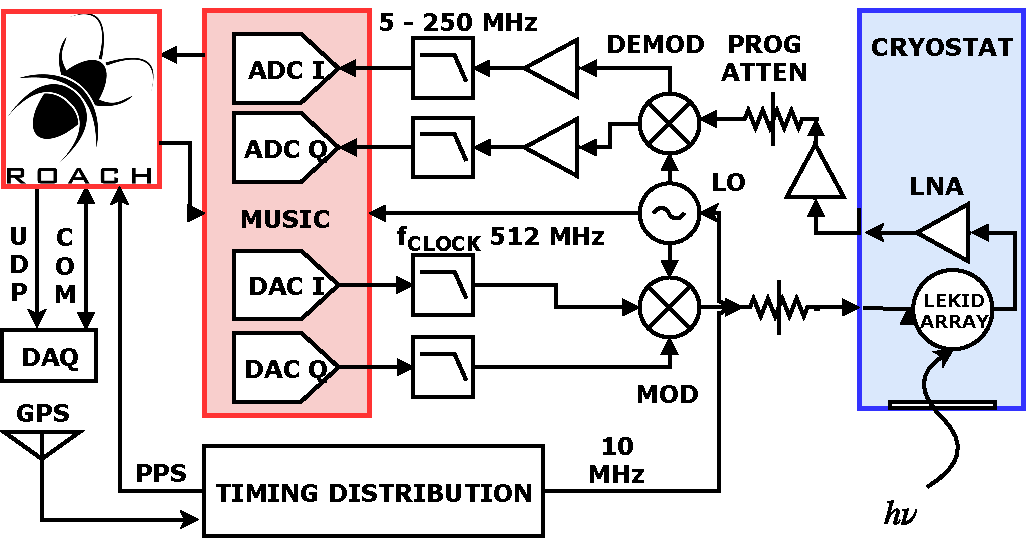
\includegraphics[width=\textwidth]{figures/readout/schematics/readoutHardwareDefense}
\caption{A schematic of the BLAST-TNG readout electronics.}
\label{fig:hw schematic}
\end{sidewaysfigure}

The primary purpose of the IF electronics is to move the signals which are produced by the ROACH2 system between complex baseband (-256 to +256~MHz) and RF ($\sim$500--1100~MHz). Additionally, the signals require amplification after passing through the cryostat. The IF electronics in each readout slice include the following components\footnote{Not included in the list: Several meters of coaxial cable; many handfuls of SMA adaptors.}:

\begin{itemize}[nosep]
  \item Four 1--256~MHz anti-aliasing filters (custom-made at ASU, one each for the $I$ and $Q$ DACs and ADCs)
  \item One quadrature modulator (Polyphase Microwave AM0350A\footnote{Polyphase Microwave:\url{https://polyphasemicrowave.com/}})
  \item One quadrature demodulator (Polyphase Microwave AD0105B)
  \item Two Mini-Circuits\footnote{Mini-Circuits:\url{https://www.minicircuits.com/}} 6000--30 programmable attenuators (steppable between 0--30~dB in 0.25~dB increments)
  \item One room-temperature (RT) LNA, (custom-made at ASU)
  \item Two RT baseband amplifiers (custom-made at ASU, one each for $I$ and $Q$ on the downconversion side.)
  \item One dual-channel synthesizer (the Valon 5009)
  \item Two 1~GHz low-pass filters (Mini-Circuits VLF-1000+, used to filter out LO harmonics and at the RF input of the readout system).
  \item Two baluns (Mini-Circuits ADT2-1T+, used to convert the single-ended $I/Q$ modulator inputs from single-ended to differential.
\end{itemize}

\vspace{5mm}

A schematic of the digital and IF electronics signal processing chain is shown in Figure~\ref{fig:hw schematic}. For explanation purposes, the signal chain can be split into two chains which merge on one end at the ROACH2 system and at the cryostat (or detector arrays) at the other.

\textit{Upconversion chain:} Starting with the ROACH-2 board, the firmware generates a baseband probe tone comb containing the resonant frequencies of each detector in the LEKID array. The signal is output in quadrature ($I$ and $Q$) by the DACs, and low-pass filtered to remove higher-order Nyquist zones (see Section~\ref{tone comb}). The signal is then upconverted to RF in the quadrature modulator, which takes the $I/Q$ quadratures as differential inputs and outputs a single RF signal. To be input into the modulator, the $I$ and $Q$ signals are converted to differential using baluns\footnote{The baluns are not required for this particular modulator. However, it is desirable to have as little LO leakage as possible at the RF output. Using baluns reduces the LO leakage to $\sim$4~dB above the probe tone level. When driven single-ended, the LO is $\sim$20~dB above the probe tones.}. The upconverted signal is then attenuated by the output-side (relative to the ROACH2) programmable attenuator before being fed into the cryostat on a single coaxial cable. The cryostat contains several temperature stages between 300~K and 300~mK, where the detector arrays are kept. Each stage contains a fixed amount of attenuation whose purpose is to reduce the thermal load on the following (colder) stages. The total gain of the cryostat depends on fixed attenuation, cable losses and LNA gain. For BLAST-TNG, the cryogenic gain is $\sim$-20~dB. After being modulated by the LEKID detectors the signal is amplified by a cryogenic 6~K LNA\footnote{A SiGe LNA from Groppi Labs at ASU\@: \url{http://thz.asu.edu/products.html}} with 30--35~dB of gain, and sent back out of the cryostat.

\vspace{5mm}

\textit{Downconversion chain:} The downconversion chain begins when the signal exits the cryostat. It is first low-pass filtered (cutoff frequency at $\sim$1~GHz) to remove any signal above $\sim$1~GHz which was amplified by the high gain of the cryogenic LNA\@. The signal then enters a second-stage amplifier, which for BLAST-TNG is a RT LNA which has been modified to operate on  5~VDC\@. The second-stage amplifier is followed by the programmable input attenuator, which feeds the demodulator. The demodulator splits the signal back into quadratures, which are passed through a third-stage of amplification that provides $\sim$20~dB of gain. The purpose of the third-stage amplifiers is to ensure that enough signal power enters the ADC when the probe tones are on resonance. The amplified quadratures are then low-pass filtered through the second pair of 1--256~MHz anti-aliasing filters, and input to the $I$ and $Q$ ADCs.

The power dissipation for each of the active IF components is listed in Table~\ref{tab:if power budget}. Their total power dissipation is $\approx$~19~W. Adding this value to the $\approx$~45~W which are dissipated by the digital electronics (Section~\ref{digital electronics}) gives a total power dissipation of $\approx$~66~W. This per-readout slice power dissipation is within acceptable range of the BLAST-TNG power requirement of $\lesssim$60~W per slice.

\begin{table}[!htbp]
\centering
\begin{tabular}{@{}lllll@{}}
\dtoprule{}
Part & Quantity & Volts (V) & Current (mA) & Total Power (W) \\ \midrule
Valon 5009 & 1 & 6 & 600 & 3.6 \\
RUDAT 6000-30 & 2 & 5 & 60 & 6 \\
Polyphase AM0350A & 1 & +5/-5 & 250/30 & 2.75 \\
Polyphase AD0540B & 1 & +5/-5 & 290/50 & 3.95 \\
RT LNA & 1 & 5 & 30 & 1.5 \\
Baseband RT Amps & 2 & 5 & 145 & 1.45 \\
 &  &  &  & 18.94 \\ \dbottomrule{}
\end{tabular}
\caption[The power dissipation for the IF electronics used in each BLAST-TNG readout slice]{The power dissipation for the IF electronics used in each BLAST-TNG readout slice}
\label{tab:if power budget}
\end{table}

\subsection{Readout Electronics for the Balloon Platform: The BLAST-TNG ROACH2 Motel}

The ROACH2 Motel, shown fully assembled in Figure~\ref{fig:roach sunset}, is a custom aluminum (Al) enclosure that houses the set of five ROACH2 readout slices, including their digital and IF electronic components. The electronics for each readout slice are mounted to 1/4$\arcsec$ backing plates, which are stacked side by side between two 5/8$\arcsec$ thick Al side panels. To allow for continuous operation at float altitude ($\sim$35~km), where fans have little effect due to the lack of atmosphere, the enclosure itself must provide a thermal link to the inner frame of the balloon gondola to enable the heat generated by the electronics to dissipate and radiate to space. Heat from each slice's backing plate flows through the two Al side panels and into two 8$\arcsec$ $\times$ 5$\arcsec$ $\times$ 1/4$\arcsec$ right angle brackets which secure the enclosure to the inner frame of the gondola (see Figure~\ref{fig:mounting roaches}). All contact joints between metal components within the enclosure are coated with non-conductive thermal joint compound to increase their thermal conductivity.

% Sunset glory
\begin{figure}[!htbp]
\centering
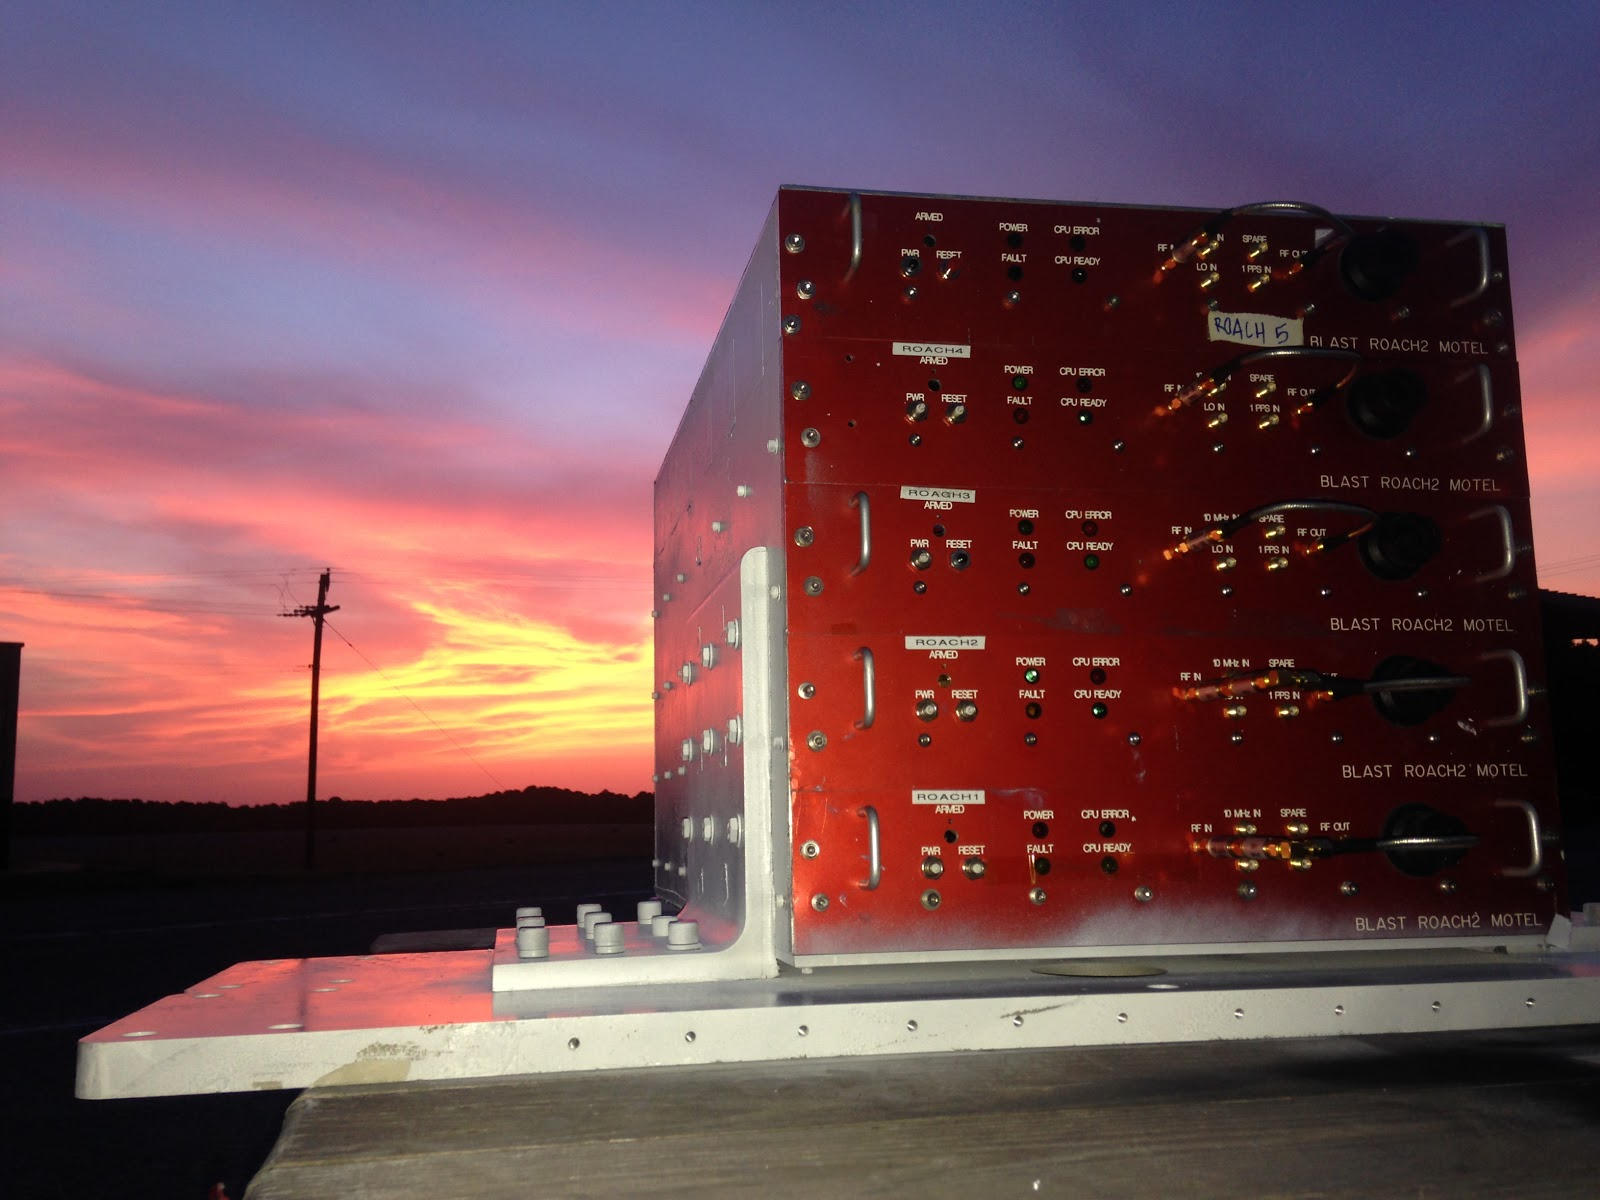
\includegraphics[width=\textwidth]{figures/readout/hardware/roach_sunset}
\caption{The BLAST-TNG ROACH2 Motel, fully assembled and taking in the sunset in Palestine, Texas, USA.}
\label{fig:roach sunset}
\end{figure}

Each of the electronics used in the BLAST-TNG detector readout are rated for operation to at least 85$^\degree$C. In order to stay within their operational temperature limits, the FPGA, PPC and ADCs must be well heat sunk to the inner plates of the enclosure, which in turn must have their own path for dissipating heat. The ROACH2's Xilinx Virtex-6 FPGA is by far the largest producer of heat in each electronics slice. To address this, a copper assembly containing two 5~mm diameter water filled, sintered copper heat pipes\footnote{Enertron Inc:\url{https://www.enertron-inc.com/}} are mounted directly on top of the FPGA chips. The heat pipes are soldered into the heat sink assemblies using bismuth tin (BiSn) solder paste. BiSn is used because its relatively low melting point of 138$^{\degree}$C allows it to liquify during fabrication without damaging the heat pipes.

% Installing ROACH2 Motel
\begin{figure}[!htbp]
\centering
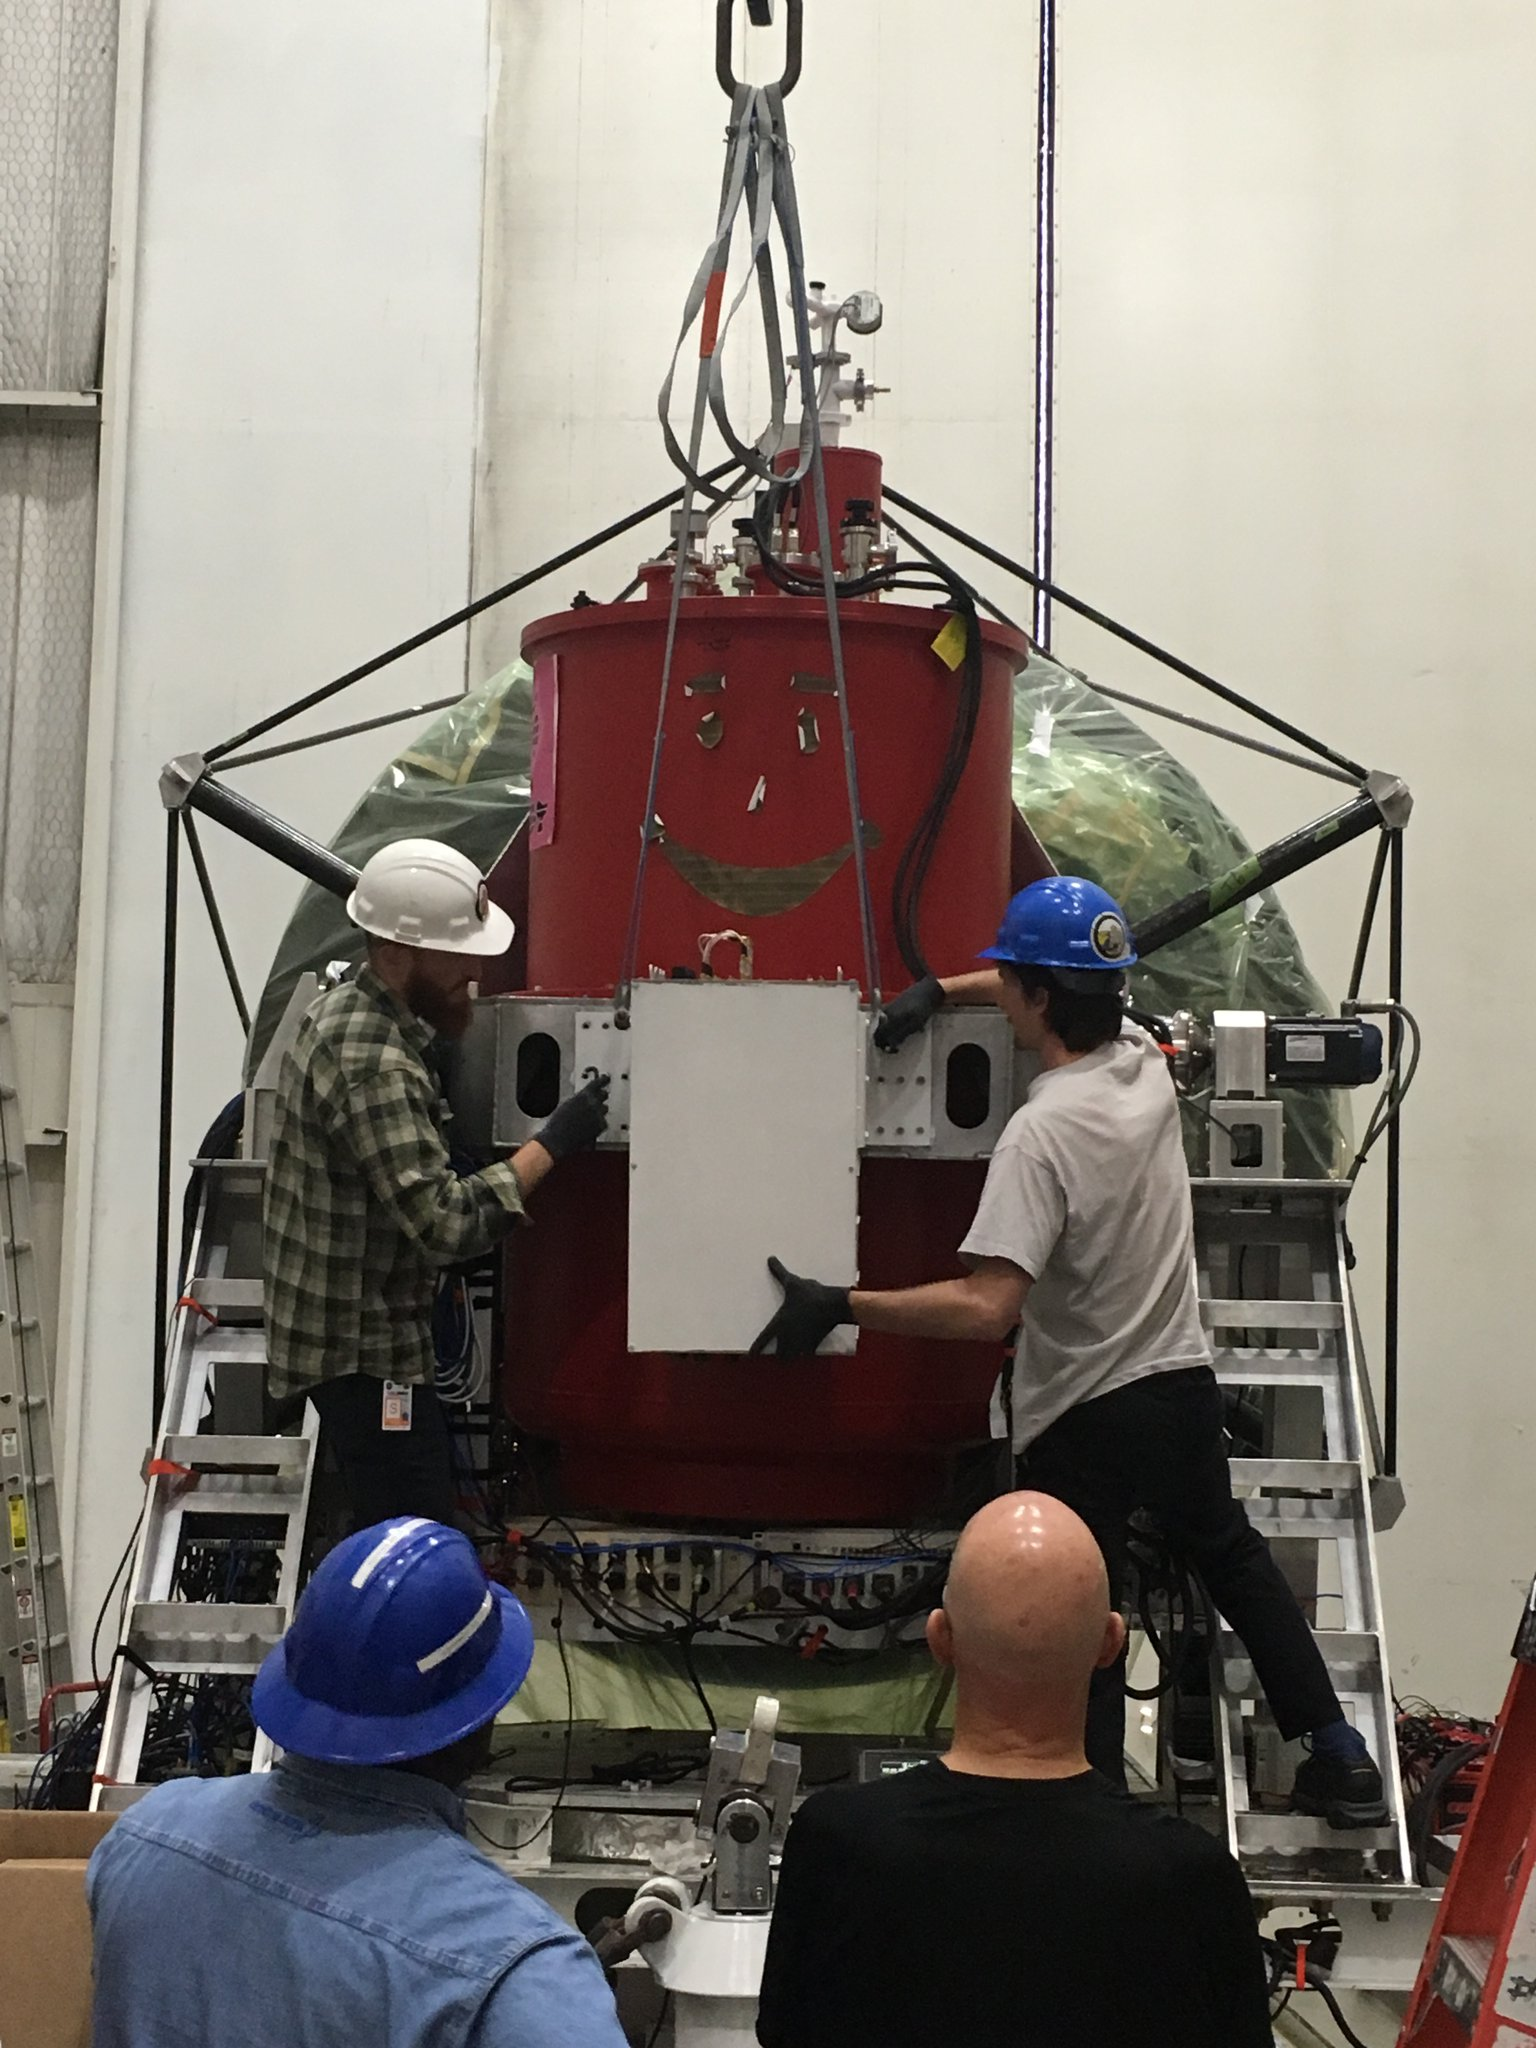
\includegraphics[width=\textwidth]{figures/readout/hardware/installing_roaches}
\caption{The `Roach Boys' installing the Roach2 Motel on the BLAST-TNG gondola in Palestine, Texas, USA (July, 2018).}
\label{fig:mounting roaches}
\end{figure}

Besides the FPGA, the two most sensitive components are the PPC and ADCs. The PPC is heat-sunk to the FPGA's heat pipe assembly using two smaller copper heat pipes, and the the ADCs are heat strapped directly to the 1/4$\arcsec$ Al backing plates using 10 AWG copper wires which are secured to the chips using non-conductive thermal epoxy. The DACs, which run cooler than the ADCs, are connected to the backing plate by a single 14~AWG copper wire. The Raspberry Pi 3 boards are mounted to Al plates which are secured to the backing plate of each slice. The IF electronics are mounted to the same backing plate as the digital electronics.

During operation of the system, the temperature of the FPGAs and PPCs is logged via temperature sensors which are secured to the heat sinking assemblies of each device. The CPU temperatures of each Raspberry Pi 3 board are also logged.

Power suppy and input and output signals are routed through the front and back panels of the ROACH2 Motel. Each slice's front panel includes SMA input ports for: A 10~MHz reference, a PPS signal, an (optional) external LO, RF input and output, and a spare input. The back panel of each slice contains a 4-pin military connector which receives 28~VDC from the balloon gondola’s power distribution system. This voltage is distributed to several Vicor\footnote{Vicor:\url{http://www.vicorpower.com}} DC-DC converters which are mounted to the enclosure's backing plate. The DC converters supply $\pm$5, 6 and 12~VDC to the IF electronics. The back panels also contain Ethernet port for communicating with the PPC, FPGA, and Raspberry Pi 3, as well as a USB port for interfacing directly with the Linux OS (BORPH) which runs on the PPC\@.

Figure~\ref{fig:if slice} is an annotated photograph of one of the five BLAST-TNG ROACH2 slices, taken during the 2018/2019 Antarctic campaign. Critical components are labeled with numbers. These are: 1) ROACH2 board 2) FPGA heat pipe assembly 3) Raspbery Pi 3 4) MUSIC DAC/ADC board 5) anti-aliasing filters 6) programmable attenuators 7) demodulator 8) modulator 9) second-stage LNA (not visible) 10) Valon synthesizer (not visible). A view of the fully assembled motel is shown in Figure~\ref{fig:top roach}. The outside of the enclosure is painted white to increase its albedo. Ethernet ports for the FPGA and PPC can be seen forming two columns that run along the back panel. The power distribution for the exposed ROACH2 slice is routed through a D-sub connector at the lower left corner of the image.

% Installing ROACH2 Motel
\begin{sidewaysfigure}[!htbp]
\centering
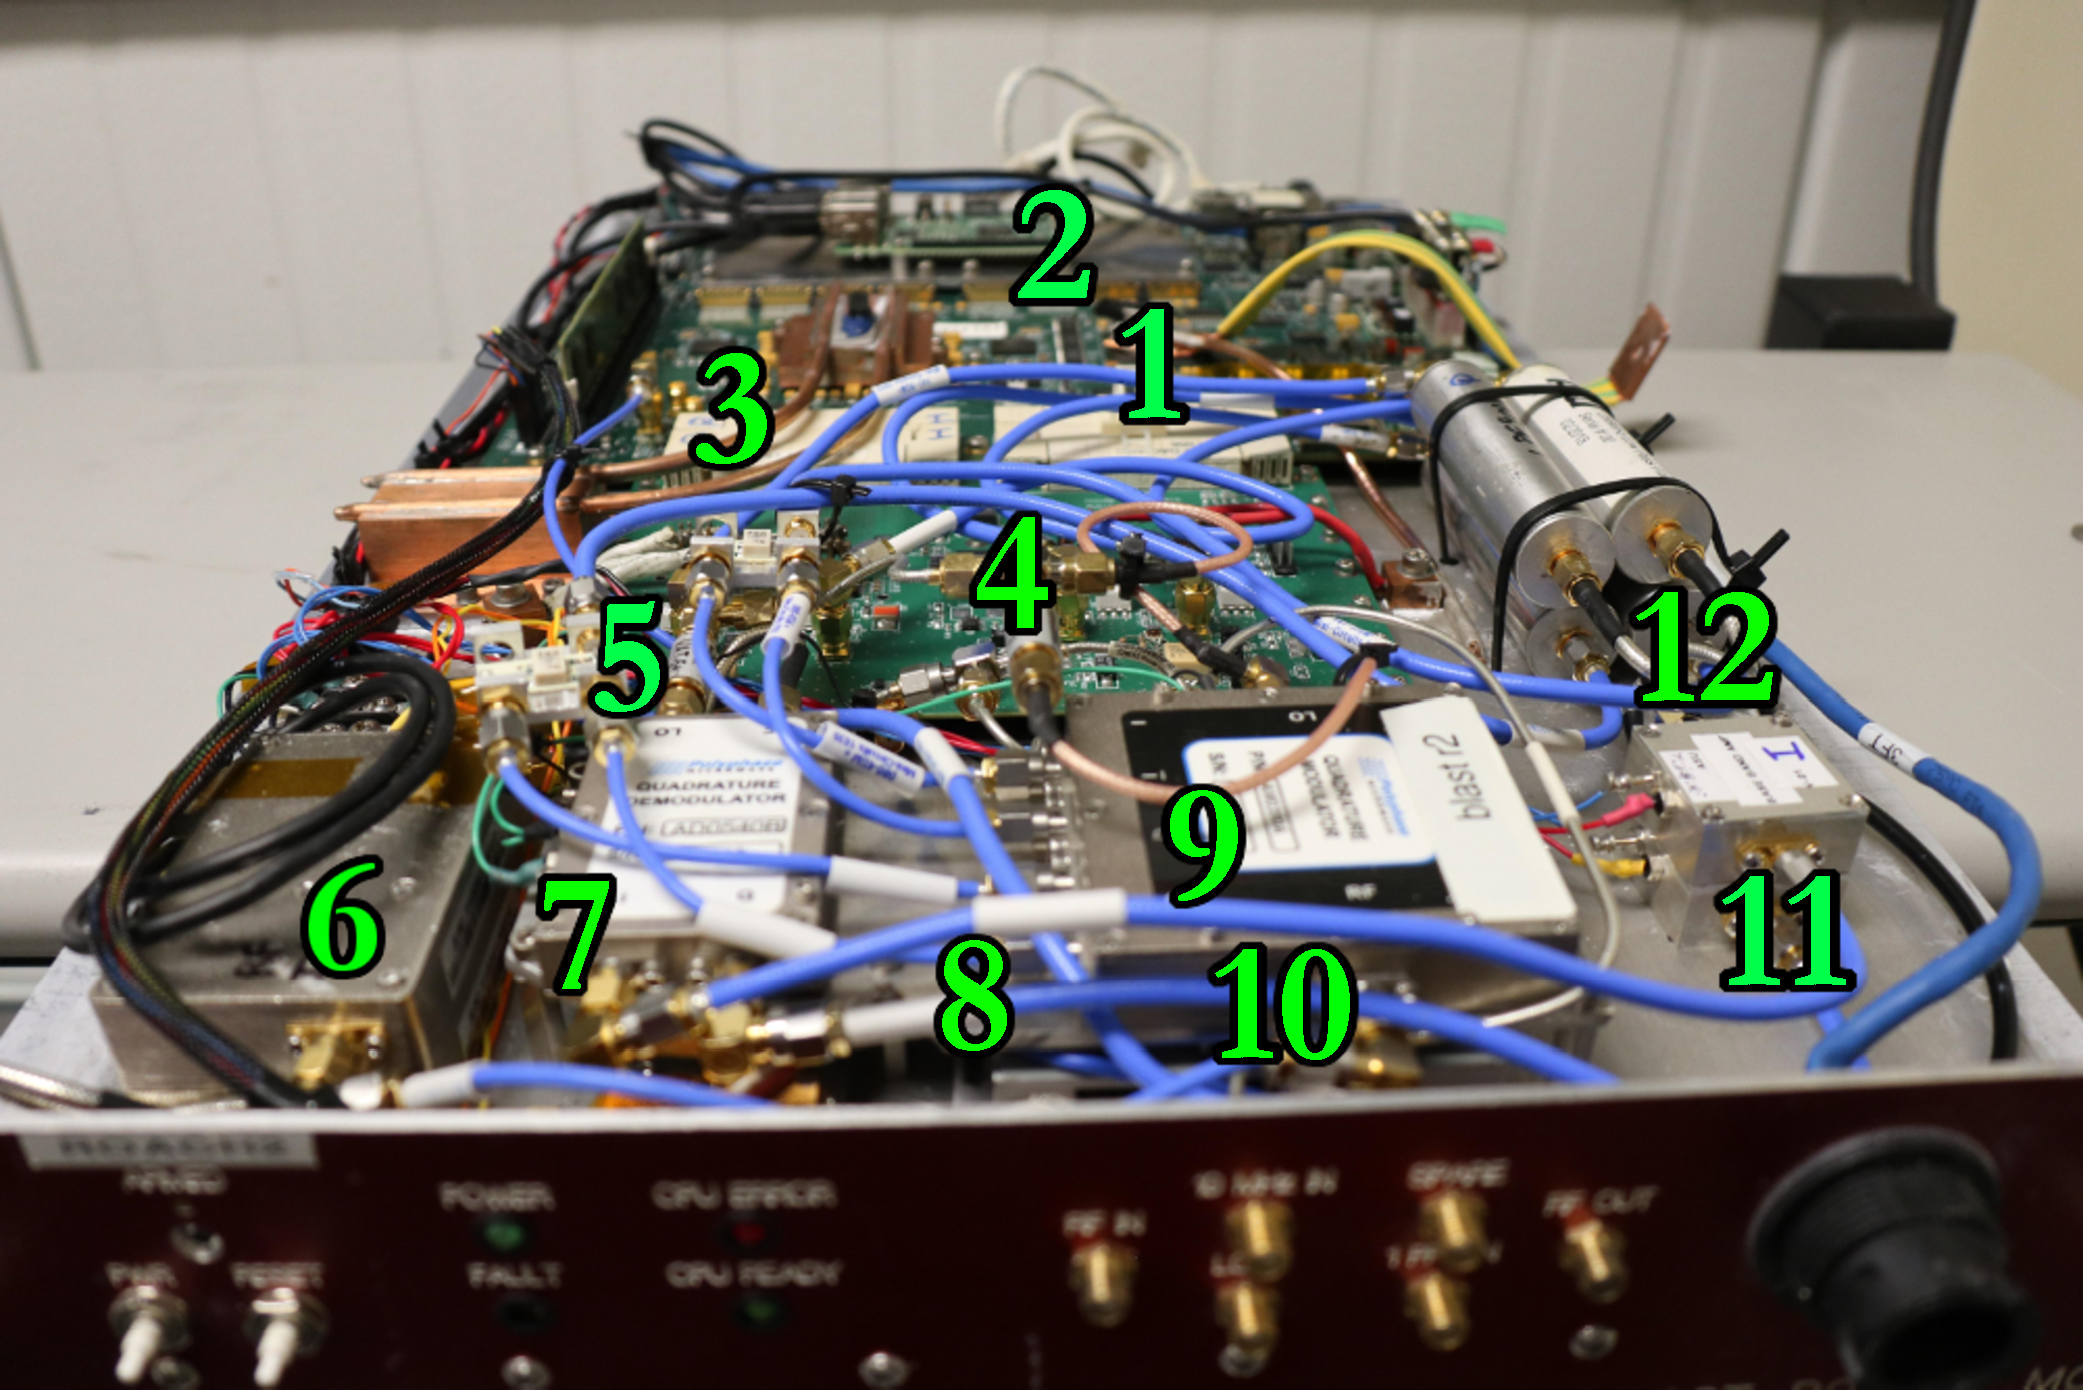
\includegraphics[width=\textwidth]{figures/readout/hardware/roach_slice_annotated}
\caption[An annotated photograph of one of the five BLAST-TNG ROACH2 electronics slices.]{An annotated photograph of one of the five BLAST-TNG ROACH2 electronics slices. Labeled components are: 1) ROACH2 board 2) Raspberry Pi 3 3) FPGA heat pipe assembly 4) MUSIC DAC/ADC board 5) baluns 6) programmable attenuators 7) demodulator 8) RT LNA (not visible) 9) modulator 10) Valon synthesizer (not visible) 11) third-stage amplifiers 12) anti-aliasing filter stack.}
\label{fig:if slice}
\end{sidewaysfigure}

% Lid open
\begin{figure}[!htbp]
\centering
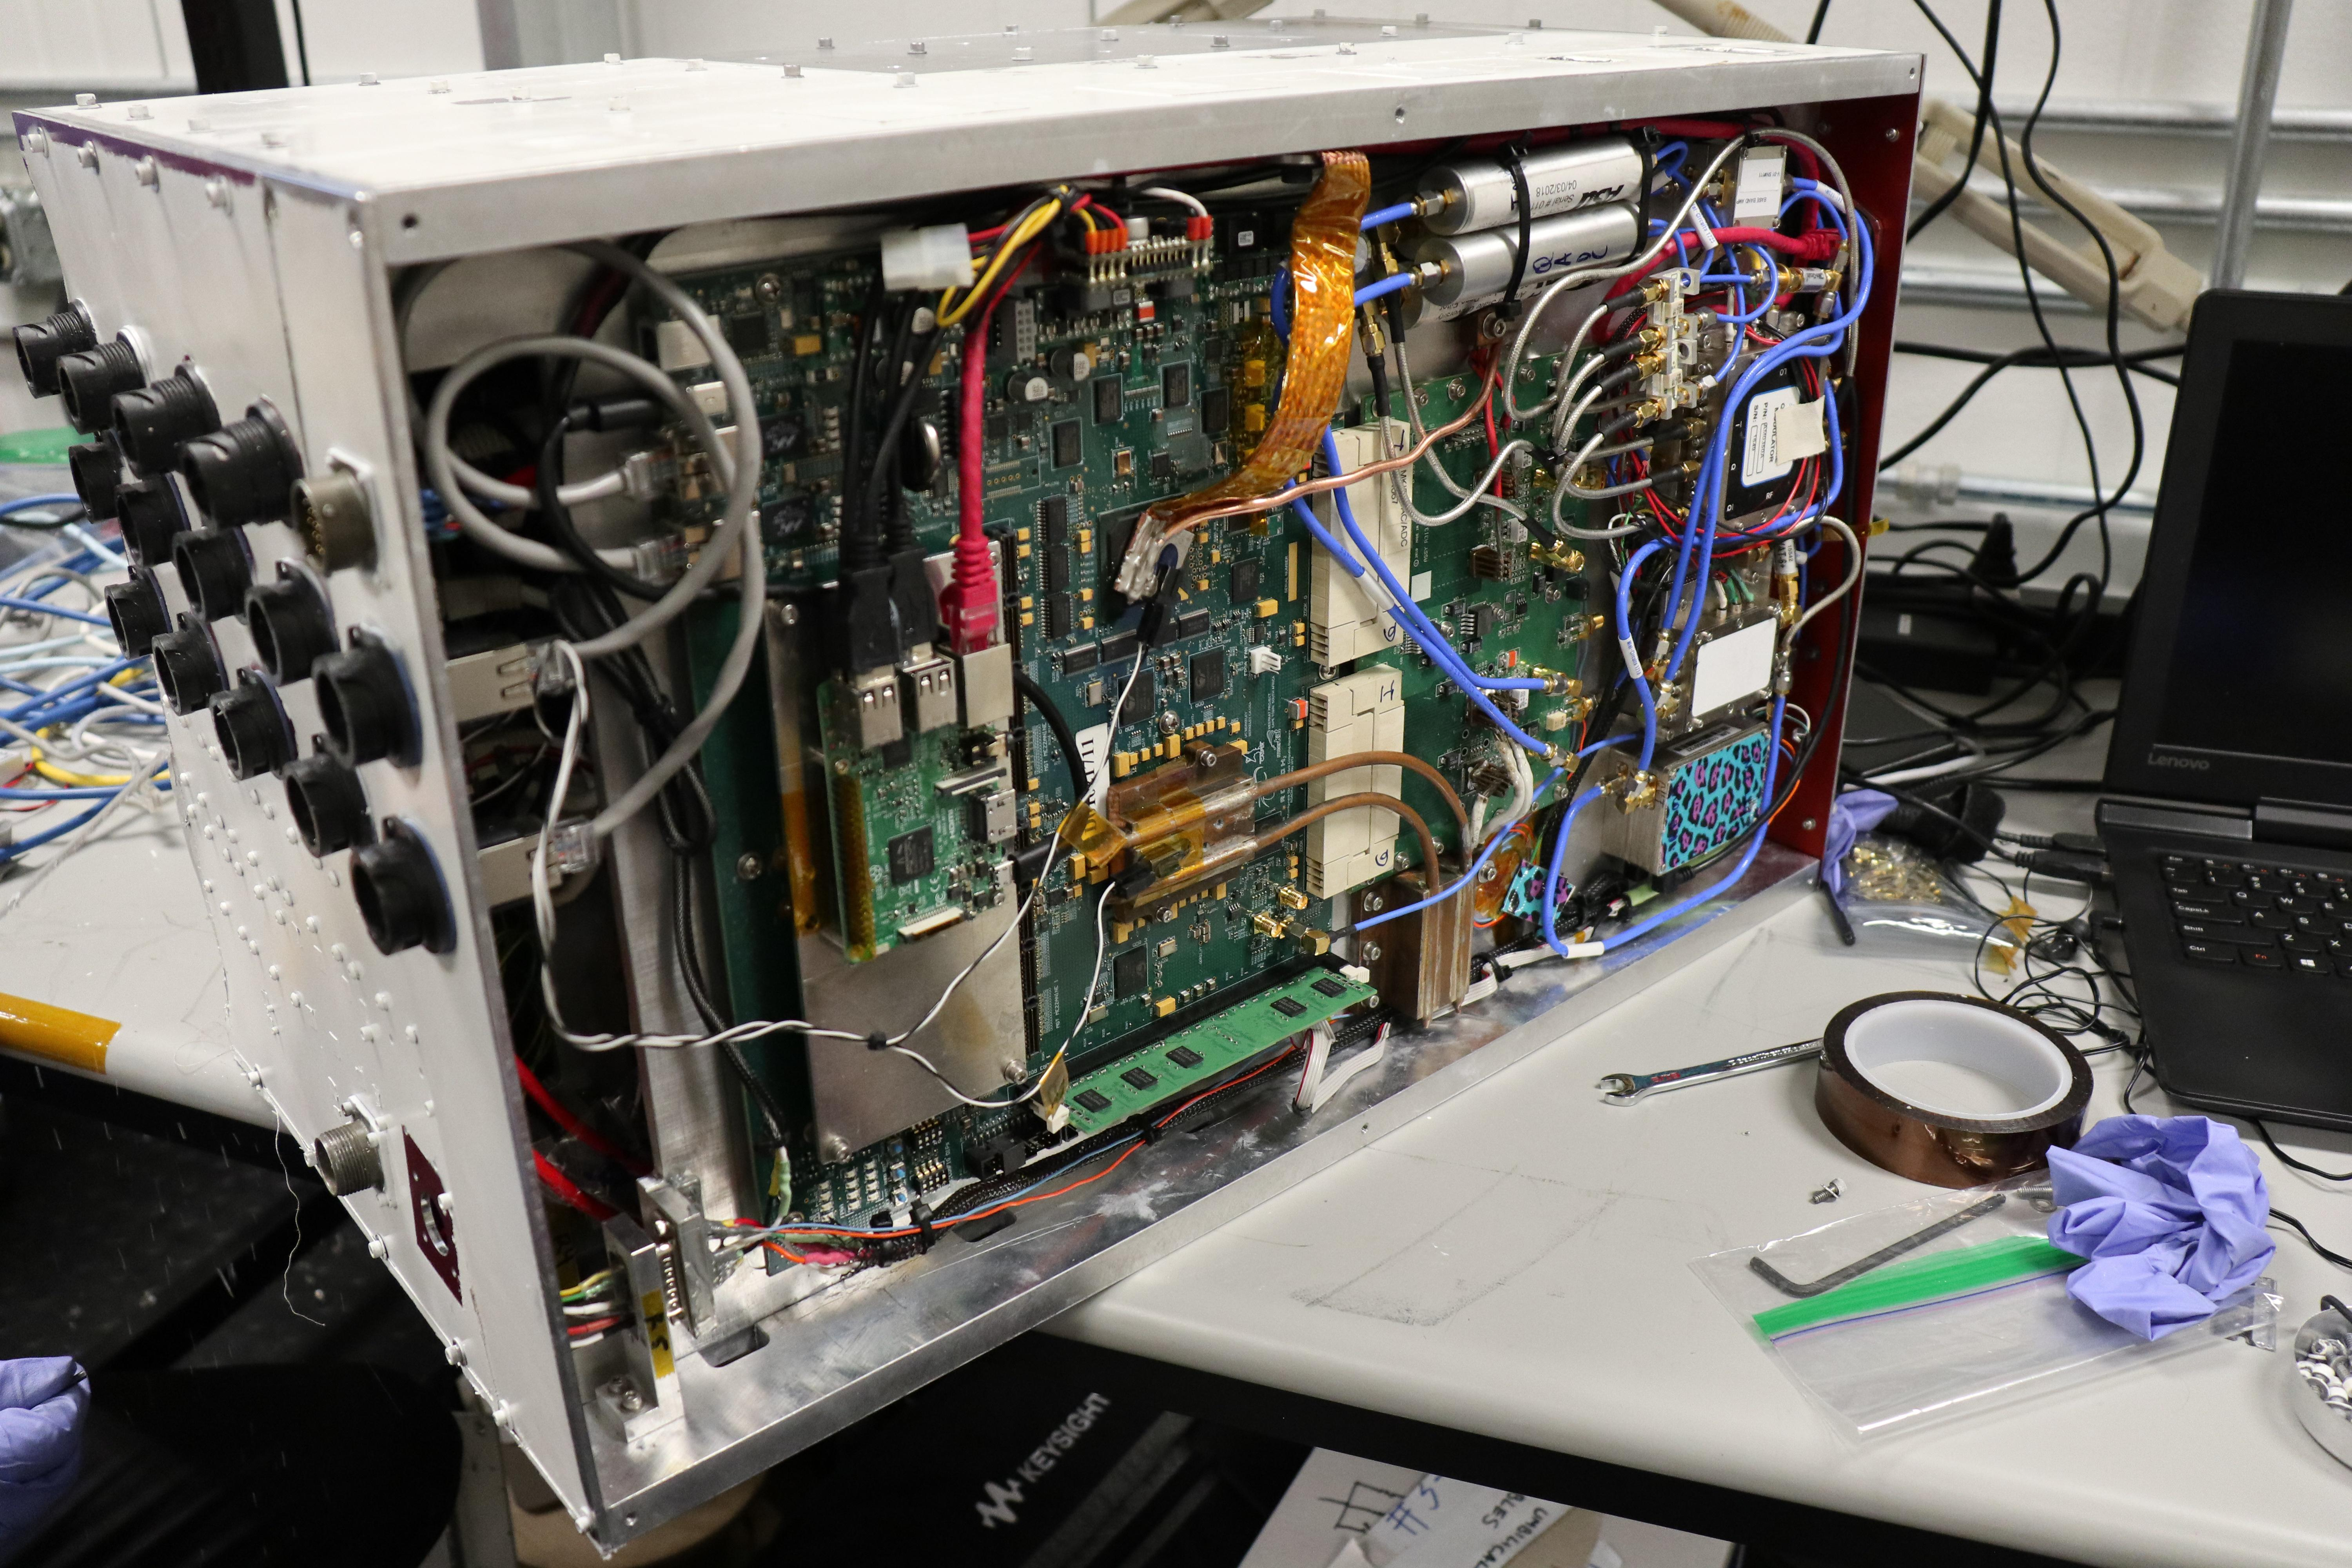
\includegraphics[width=\textwidth]{figures/readout/hardware/roach_motel_open}
\caption[A top view of the BLAST-TNG ROACH2 Motel, with the lid removed.]{A top view of the BLAST-TNG ROACH2 Motel, with the lid removed.}
\label{fig:top roach}
\end{figure}

\begin{comment}
\begin{figure}[!htbp]
\centering
\includegraphics[width=\textwidth]{figures/readout/minicircuitsLPFcomp_crop}
\caption{Comparison of the simulated S21 (ASU, red), measured S21 (ASU, black) and measured S21 (Minicircuits, blue).}
\label{fig:lpf comp}
\end{figure}

\begin{figure}[!htbp]
\centering
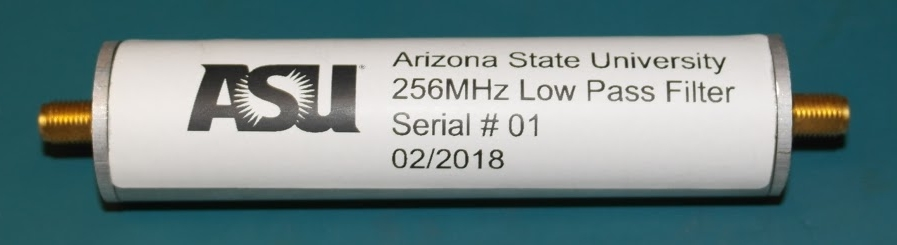
\includegraphics[width=\textwidth]{figures/readout/lpf_tube}
\caption{Comparison of the simulated S21 (ASU, red), measured S21 (ASU, black) and measured S21 (Minicircuits, blue).}
\label{fig:lpf}
\end{figure}

\begin{figure}[!htbp]
\centering
\includegraphics[width=\textwidth]{figures/readout/activeFilterbox_crop}
\caption{Comparison of the simulated S21 (ASU, red), measured S21 (ASU, black) and measured S21 (Minicircuits, blue).}
\label{fig:activeFilter}
\end{figure}

\begin{figure}[!htbp]
\centering
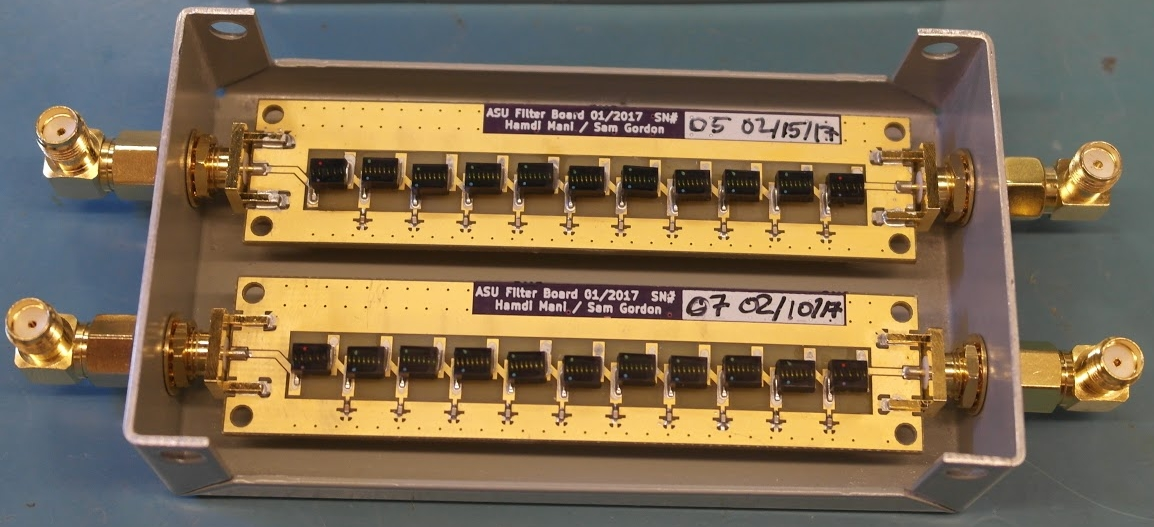
\includegraphics[width=\textwidth]{figures/readout/dac_lpf_crop}
\caption{Comparison of the simulated S21 (ASU, red), measured S21 (ASU, black) and measured S21 (Minicircuits, blue).}
\label{fig:dacLPF}
\end{figure}

\begin{figure}[!htbp]
\centering
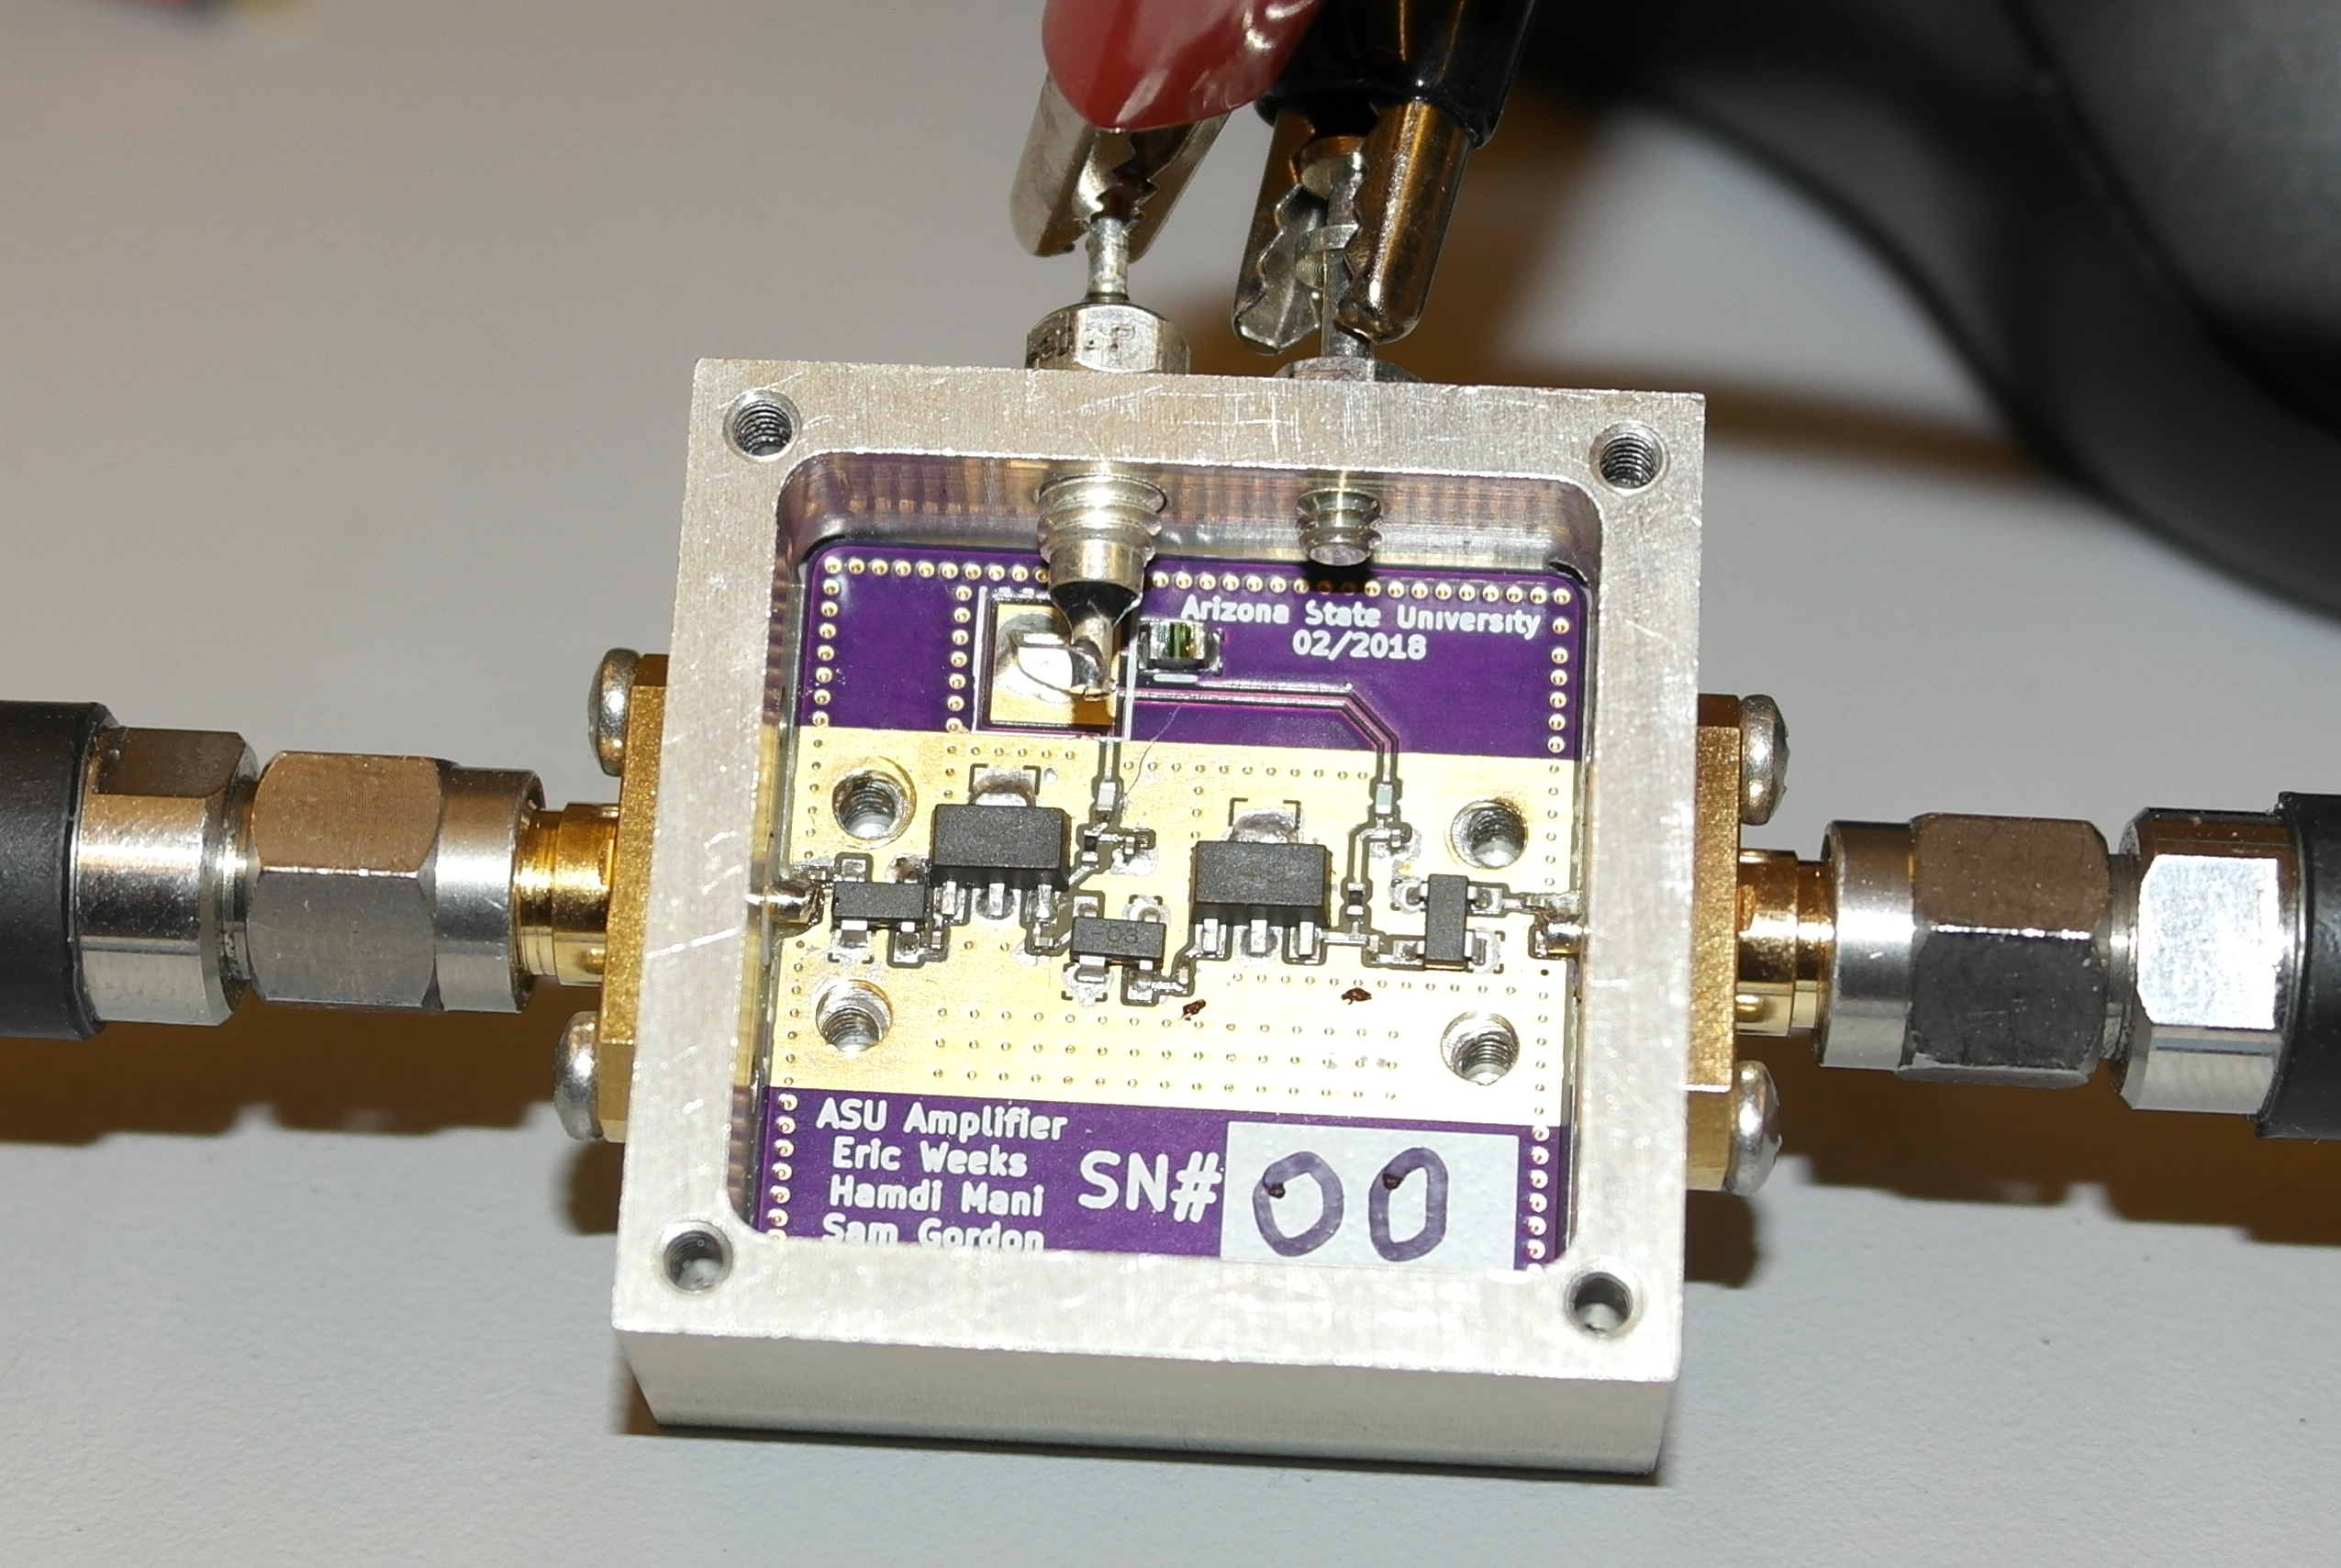
\includegraphics[width=\textwidth]{figures/readout/bb_amp_00_crop}
\caption{Comparison of the simulated S21 (ASU, red), measured S21 (ASU, black) and measured S21 (Minicircuits, blue).}
\label{fig:bb_amp_00}
\end{figure}
\end{comment}

\section{ROACH2 Firmware Overview}\label{firmware}

In this section we describe in detail the DSP which is performed in the FPGA firmware. The firmware is written using the MATLAB\footnote{Mathworks:\url{https://www.mathworks.com/}} / Simulink\footnote{Mathworks} / System Generator\footnote{Xilinx ISE 14.7 Design Suite} / EDK\footnote{Xilinx Embedded Development Kit} (MSSGE) Toolflow developed by the CASPER collaboration. CASPER `snap' blocks allow for pre-specified amounts of data from the data stream to be saved in block RAM (BRAM) on the FPGA at key points in the DSP chain. This data can then be converted into figures of merit to be used for making real-time adjustments to either the RF electronics or baseband frequency combs. Critical parameters, including the readout bandwidth, may be adjusted during operation using software inputs.

The DSP chain performs several synthesis and analysis functions, which are described sequentially in the sections below. A block diagram of the DSP chain is shown in Figure~\ref{fig:DSP schematic}.

% DSP flow
\begin{sidewaysfigure}[!p]
\centering
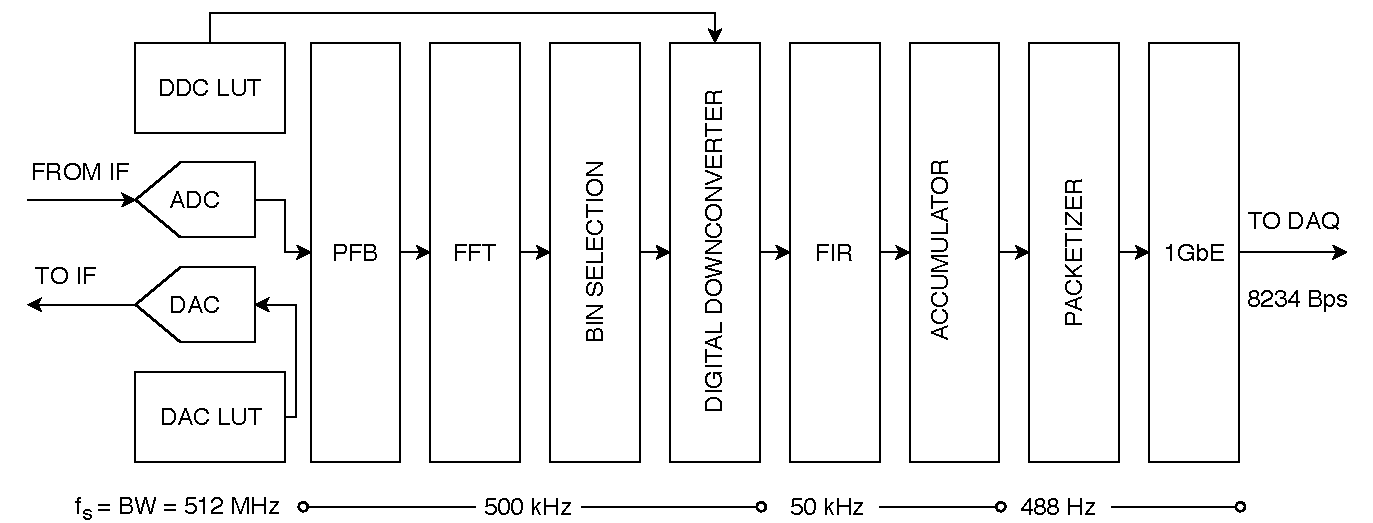
\includegraphics[width=\textwidth]{figures/readout/schematics/readoutDSPdiagram}
\caption{A schematic of the firmware DSP chain.}
\label{fig:DSP schematic}
\end{sidewaysfigure}

\subsection{Tone Comb Synthesis}\label{tone comb}

The DSP chain begins with the synthesis of the DAC probe tone and DDC tone look-up-tables (LUTs). The DDC tones are used to digitally downconvert the output timestreams of the PFB-FFT (see Section~\ref{ddc}), and the DAC probe tones circulate between the readout system and the LEKID arrays throughout an observation. If the resonator frequencies are not known, they can be discovered using the channel identification technique described in Section~\ref{KID-finding}. In the following, we assume that the LEKID resonant frequencies ($f_{\mathrm{res}}$) are already known.

The time domain waveform of the DAC probe tone is synthesized in software (\texttt{Python/C/C++}) by assembling a dummy spectrum in the frequency domain, and then taking its inverse-Fourier transform (IFT). In the dummy spectrum, each probe tone is represented by an amplitude $A$ and unique phase $\phi$. During an observation, the probe tone amplitudes are set to unique values corresponding to the specific tone power requirements of the detectors (including a global transfer function correction to correct for the ROACH2-output side IF electronics, described in Section~\ref{TRF}). In the examples which are provided in the following, the tone amplitudes are normalized to their maximum allowable value, which is 32767 analog-digital units (ADU). At the DAC output, this level corresponds to $V_{pp} \simeq 1.4$~V.

The phases of the probe tones are chosen from a normal distribution. This produces a near-optimal CF for a multitone comb with an arbitrary number of tones (\citet{boyd1986multitone}). The tone frequencies occupy the complex baseband bandwidth of the ROACH2/MUSIC board system, which spans from -256 to +256~MHz (for a good explanation of negative frequency, see \citet{lyons2004understanding}). The tone frequencies are rounded to increments of the final channelizer bandwidth of 488.28125~Hz.

The DDC tones are computed in a similar fashion as the DAC tones, although their frequencies correspond to the difference between the DAC probe tone frequencies and the center frequencies $f_{k}$ of their firmware FFT bins. For a given FFT bin index $k$, $f_{k} = kf_{s}/N_{\mathrm{FFT}}$. The frequency of the DDC tone corresponding to a probe tone at frequency $f_{\mathrm{pr}}$ which is located in bin $k$ is therefore $f_{k,\mathrm{DDC}} = f_{\mathrm{pr}} - f_{k}$. The sampling frequency for the DDC LUT is the PFB-FFT output frequency, $f_{\mathrm{FFT}} = 500$~kHz.

Once synthesized in software, the DAC and DDC comb LUTs are uploaded to the ROACH2 board, where they occupy two of the ROACH2's four quad-data-rate (QDR) SRAM chips\footnote{Cypress, CY7C2565KV18}, hereafter designated QDR$_{I}$ and QDR$ _{Q}$. Each LUT contains 2$^{21}$ signed 16-bit time ordered samples.

The QDR is logically accessed as 2$^{19}$ addresses $\times$ 16-B. The KATCP protocol is used to upload the LUT data to QDR RAM\@. To facilitate uploading the two LUTs to each QDR, the $I$ and $Q$ components are interwoven into two separate LUTs (LUT$_{I}$, LUT$_{Q}$) of 2$^{22}$ time ordered samples each (this is based on the method used by \citet{mchugh2012readout}). For example, the order of samples contained within LUT$_{I}$ is:

\begin{equation} I_{\mathrm{DAC}}^{1}, I_{\mathrm{DAC}}^{0}, I_{\mathrm{DDC}}^{1},I_{\mathrm{DDC}}^{0}, \ldots , I_{\mathrm{DAC}}^{n}, I_{\mathrm{DAC}}^{n - 1 }, I_{\mathrm{DDC}}^{n}, I_{\mathrm{DDC}}^{n - 1} \end{equation}
where superscripts refer to even and odd numbered samples, and each value is 16-bit wide.

After the LUTs have been uploaded to the QDRs, they are read from the QDR buffers, sliced into their original 16-bit values and re-cast as fixed-point 16.15 values\footnote{In this fixed-point notation, the first number represents the total bit width, with the second number being the radix point. All numbers in this notation are assumed to be signed unless otherwise noted.}. On each clock cycle, four consecutive samples are read out from QDR$_{I}$ (QDR$_{Q}$): $I_{\mathrm{DAC}}^{1}, I_{\mathrm{DAC}}^{0}, I_{\mathrm{DDC}}^{1}, I_{\mathrm{DDC}}^{0}$ (same for $Q$).

The DDC LUT samples are sent directly to the DDC section of the firmware, while the DAC LUT samples are input to the MUSIC board DAC gateware. Since the DACs are clocked at twice the rate of the FPGAs, two consecutive samples (e.g., $I_{\mathrm{DAC}}^{1}, I_{\mathrm{DAC}}^{0})$ are processed on each FPGA clock cycle. To ensure proper synchronization of each quadrature component, the DAC is synchronized by a pulse which simultaneously resets the QDR address counter.

Because the DAC waveforms are reconstructed using a zero-order hold (ZOH), the frequency response of the waveform is a sinc function: $\mathcal{X}(f) = \left|{\mathrm{sinc}}(\pi f/f_{s}) \right|$. The sinc response produces two effects which must be considered individually. The first effect is a roll-off of $\sim$6~dB between the center of the band and the edge of the first Nyquist zone, at $f_{\mathrm{FPGA}} = 256$~MHz. This roll-off is dealt with by applying an inverse transfer function correction to the probe tone amplitudes.

The second consequence of the ZOH is that several higher order Nyquist zones are output by the DAC, which must be removed using high-order low-pass filters. Figure~\ref{fig:dac sim} shows the measured output of one DAC for a tone comb comprised of 1,000 evenly spaced tones, ranging from -245--245~MHz. The blue trace is the unfiltered frequency response out to 1.5~GHz. The power in the second Nyquist zone ($f_{s}$---$\frac{3}{2}f_{s}$) is $\sim$10~dB below the peak at $f \simeq 250$~MHz. The orange trace shows the simulated sinc response. The simulation is a good match the first Nyquist zone, but does not taper off at higher zones (no frequency dependent attenuation factor was included in the simulation). The red trace shows the DAC output after the application of the anti-aliasing filters, which cut off at $\sim$245~MHz.

\begin{figure}[!htbp]
\centering
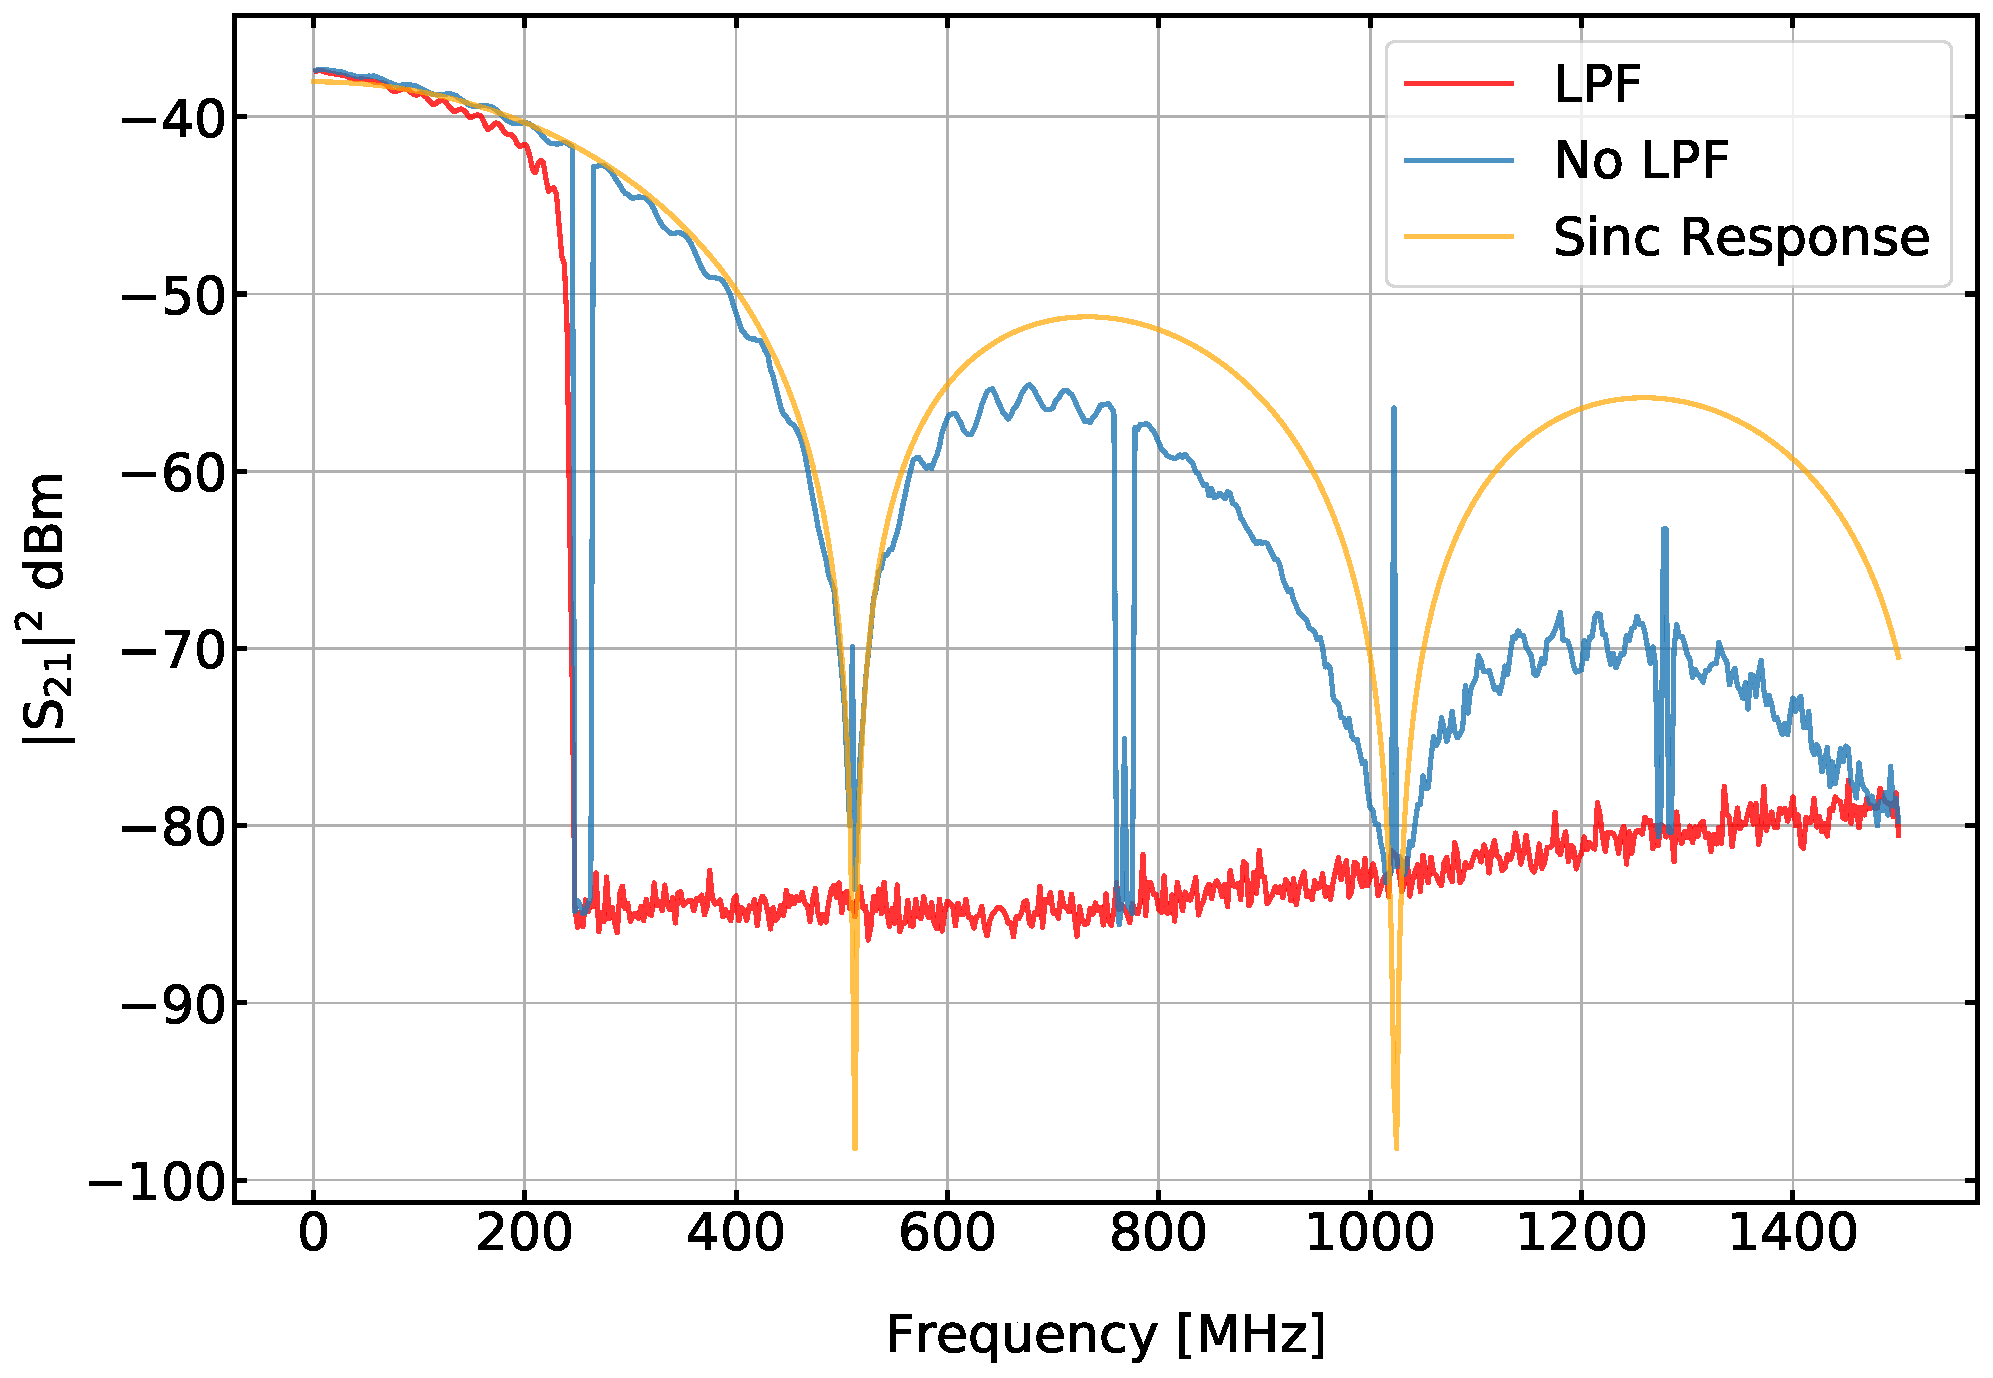
\includegraphics[width=\textwidth]{figures/readout/sim/dac_comp}
\caption[The DAC frequency response (measured and simulated), with and without anti-aliasing filters.]{The DAC frequency response for a multitone probe comb with $N = 1000$, showing the unfiltered (blue), simulated (orange) and measured filtered (red) response out to 1.5~GHz.}
\label{fig:dac sim}
\end{figure}

\subsection{Digitization}\label{digitization}

After the tone comb has been upconverted by the IF electronics, passed through the detector arrays, and once again downconverted to complex baseband, the $I$ and $Q$ signals are digitized by two independent ADCs which share the same clock source as the DACs. Each ADC outputs two consecutive time samples per FPGA clock cycle: I$_{\mathrm{ADC}}^{1}$, I$_{\mathrm{ADC}}^{0}$ (Q$_{\mathrm{ADC}}^{1}$, Q$_{\mathrm{ADC}}^{0}$). The time ordered $I/Q$ pairs are concatenated and sent to the first stage of channelization, which is the PFB-FFT\@. CASPER snap blocks are utilized at this stage to store some of the ADC timestream in BRAM, which can be downloaded to the DAQ at any time in order to calculate $V_{\mathrm{rms}}$ at the ADC input for both $I$ and $Q$. The ADCs have a full-scale input range of 1.1~V, which corresponds to a maximum allowable input power of 10.8~dBm.

Figure~\ref{fig:adc} shows 2,000 samples of the digitized timestream of a single tone at $f_{\mathrm{pr}} = 50.0125$~MHz, as well as for a tone comb with $N_{\mathrm{tones}} = 1000$ with evenly spaced frequencies. The power in the single tone has been attenuated using the output attenuator inside the IF electronics, to avoid saturating the ADCs. Because the phases of the multitone comb are randomized, the peak power in the comb scales as $P_{\mathrm{max}} \propto \sqrt{N_{\mathrm{tones}}}$. During an observation, the IF attenuators are adjusted to keep the RMS voltage of the tone comb to below $\approx$~100~mV. This ensures that the ADC will not saturate as the LEKID resonant frequencies drift from the initial locations of the probe tones, increasing their transmission through the system.

The CF of the waveform can also be measured from a small number of ADC samples, for both $I$ and for $Q$. For the data shown in Figure~\ref{fig:adc}, the CF is measured as 3~dB for the single tone, and 11.3~dB for the 1,000 tone comb. The real-time CF measurements are useful for making noise estimates (see Section~\ref{noise verify}).

% ADC
\begin{figure}[!htbp]
\centering
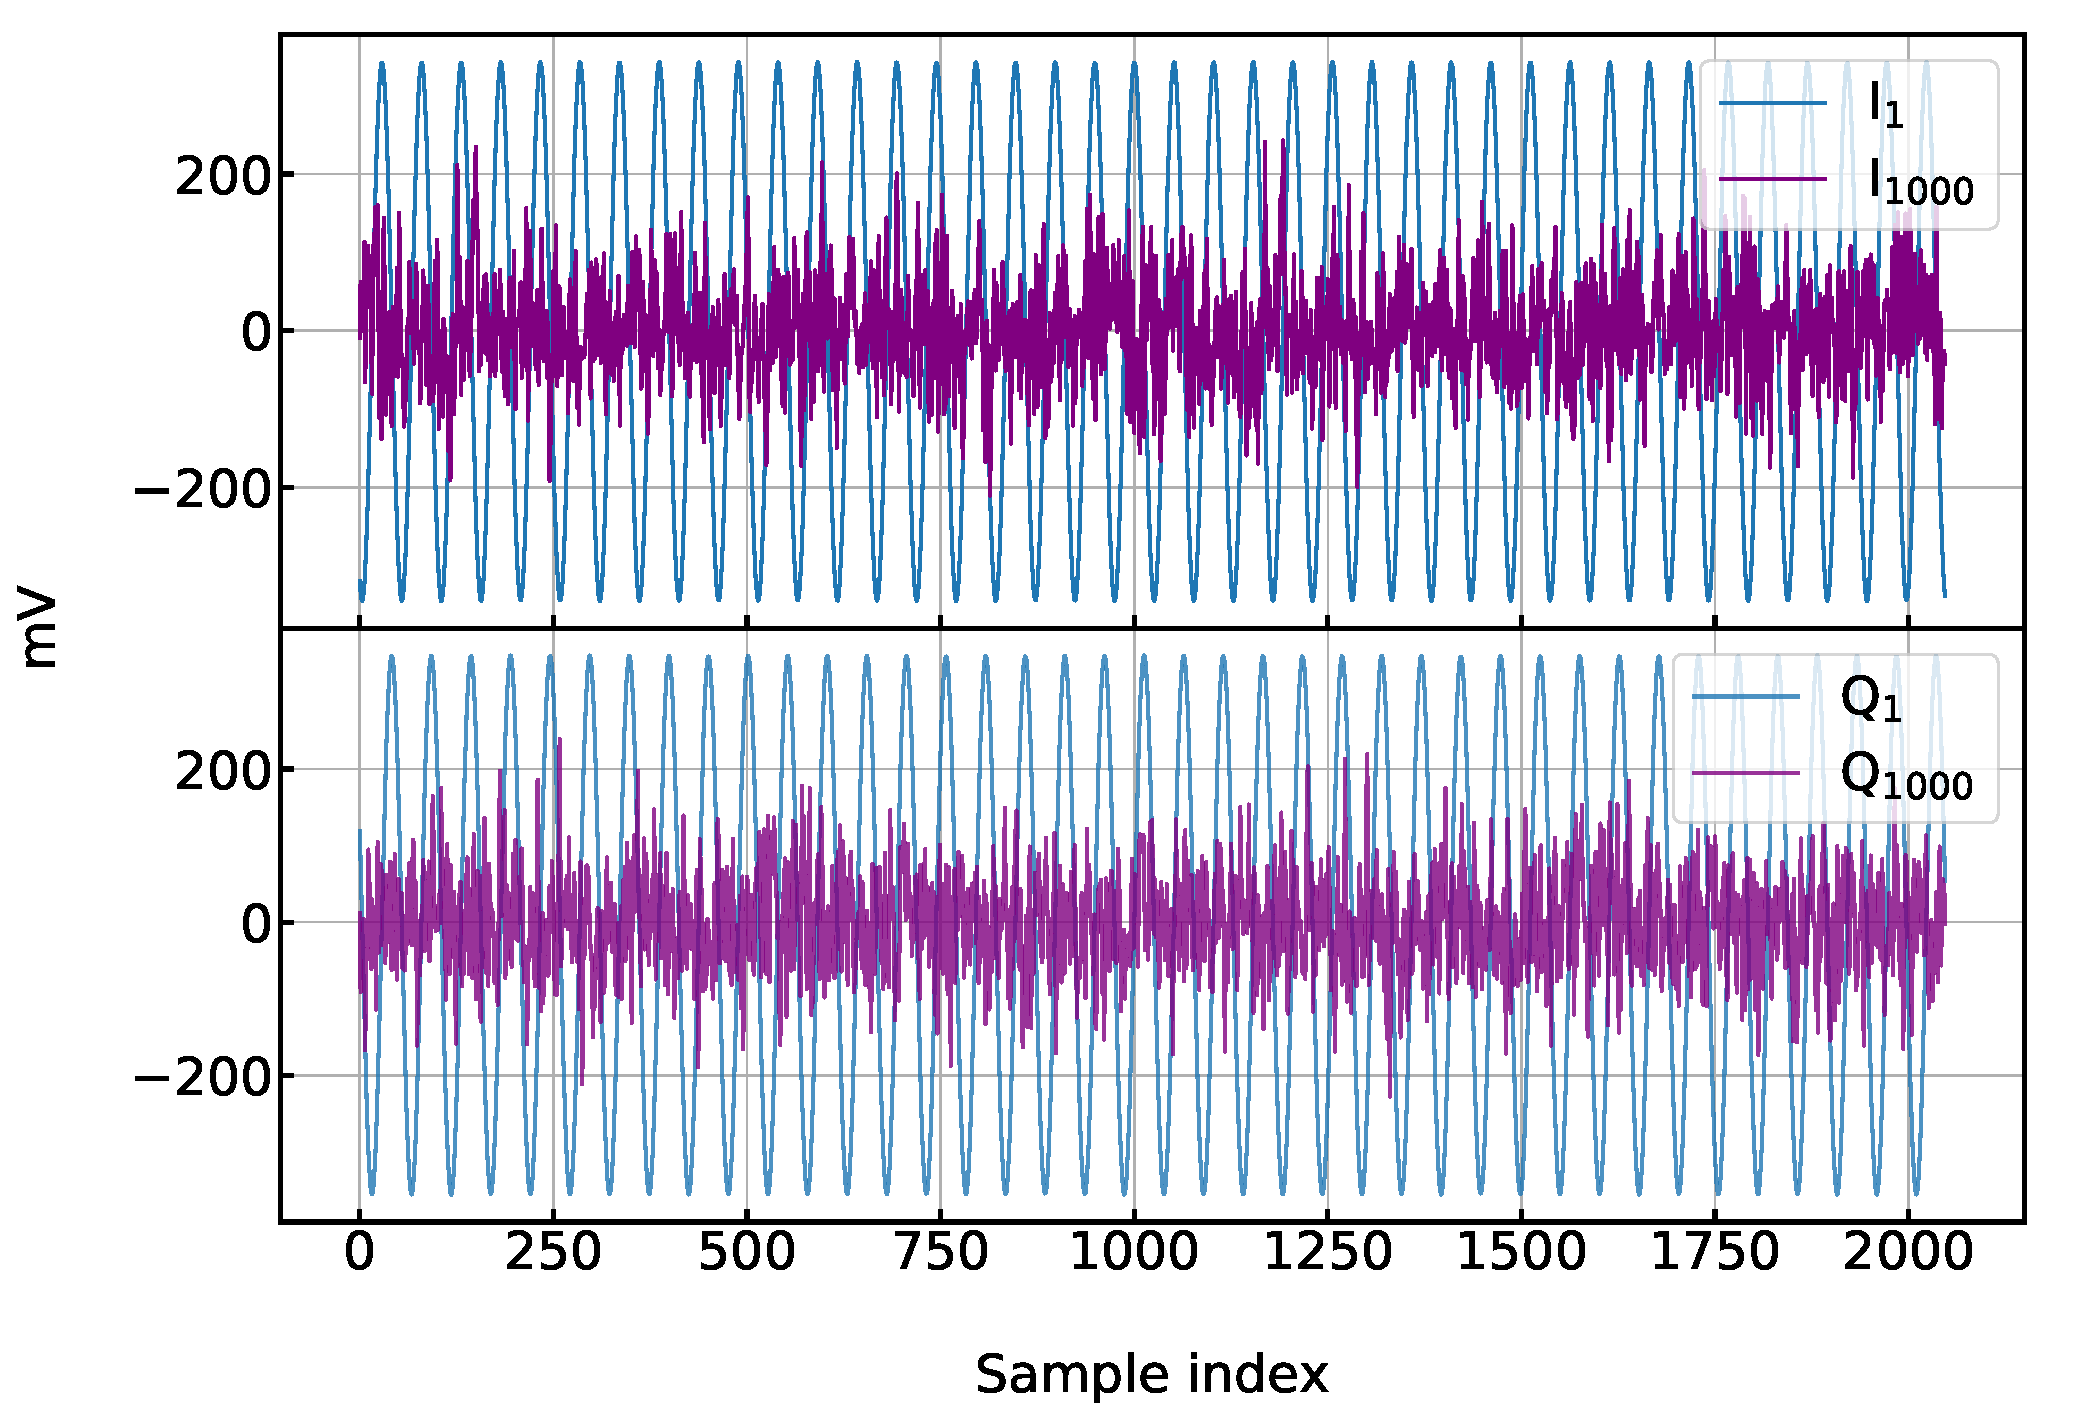
\includegraphics[width=\textwidth]{figures/readout/sim/adc}
\caption[2,000 \macrocapwrap{$I/Q$} samples of a digitized waveform for a single tone at f = 50.0125~Hz, and 1,000 evenly spaced tones.]{2,000 \macrocapwrap{$I/Q$} samples of a digitized waveform at \macrocapwrap{$f = 50.0125$}~Hz (blue), and for a tone comb consisting of 1,000 evenly spaced tones.}
\label{fig:adc}
\end{figure}

\subsection{Coarse Channelization: The PFB-FFT}\label{pfb}

Inside the firmware, the digitized tone comb is processed using two consecutive stages of channelization. The first stage of channelization is a PFB-FFT (AKA filterbank). A detailed description of PFBs is found in \citet{price2016spectrometers}. Utilizing a PFB before an FFT allows for frequency response of the FFT bins to be shaped according to the chosen PFB parameters. Specifically, the PFB is intended to minimize the two most deleterious side-effects of FFTs, which are spectral leakage and scalloping loss.

A PFB accomplishes this by multiplying a segment of timestream (for either $I$ or $Q$) with a window function, dividing the windowed segment into $P$ `phases' of length $N_{\mathrm{FFT}}$ (the poly-phases), and summing each of the $P$ phases. The summed segment of length $N_{\mathrm{FFT}}$ is then fed into a FFT, also of length $N_{\mathrm{FFT}}$ (the PFB-FFT is the combination of the two). The PFB acts as a set of sub-filters which condition the FFT bin transfer functions so that they are more rectangular than they would be otherwise. Lower sidelobe levels can be achieved by widening the the FFT bins.

The PFB-FFT is implemented using the CASPER \texttt{pfb\_fir} and \texttt{biplex\_fft} blocks. For the PFB, we use a $P = 4$ taps, a bin scaling factor of 2, and a Hamming window for the filter coefficients. The bin scaling factor of 2 widens the FFT bins so that they overlap at -6~dB. Their width at FWHM is 450~kHz. On each clock cycle, the biplex FFT receives two consecutive complex time ordered samples $I_{0}, I_{1}, Q_{0}, Q_{1}$, and outputs the complex amplitudes $\widetilde{I}_{0}, \widetilde{I}_{1}, \widetilde{Q}_{0}, \widetilde{Q}_{1}$ of two consecutive ($k$, $k + 1$) frequency bins. One $N = 1024$ FFT is processed every 512 clock cycles, corresponding to an FFT-rate of 500~kHz. A synchronization pulse which is emitted on the last clock cycle before the first valid data of each consecutive FFT is used to synchronize all following stages of the firmware. Since the average individual detector bandwidth is $\sim$50~kHz, several detectors may safely fall within a single FFT bin. Each bin pair output by the FFT is concatenated into a single 72-bit word (4 $\times$ 18-bit) before being stored in block RAM (BRAM) in the FPGA for channel selection.

\begin{figure}[!htbp]
\centering
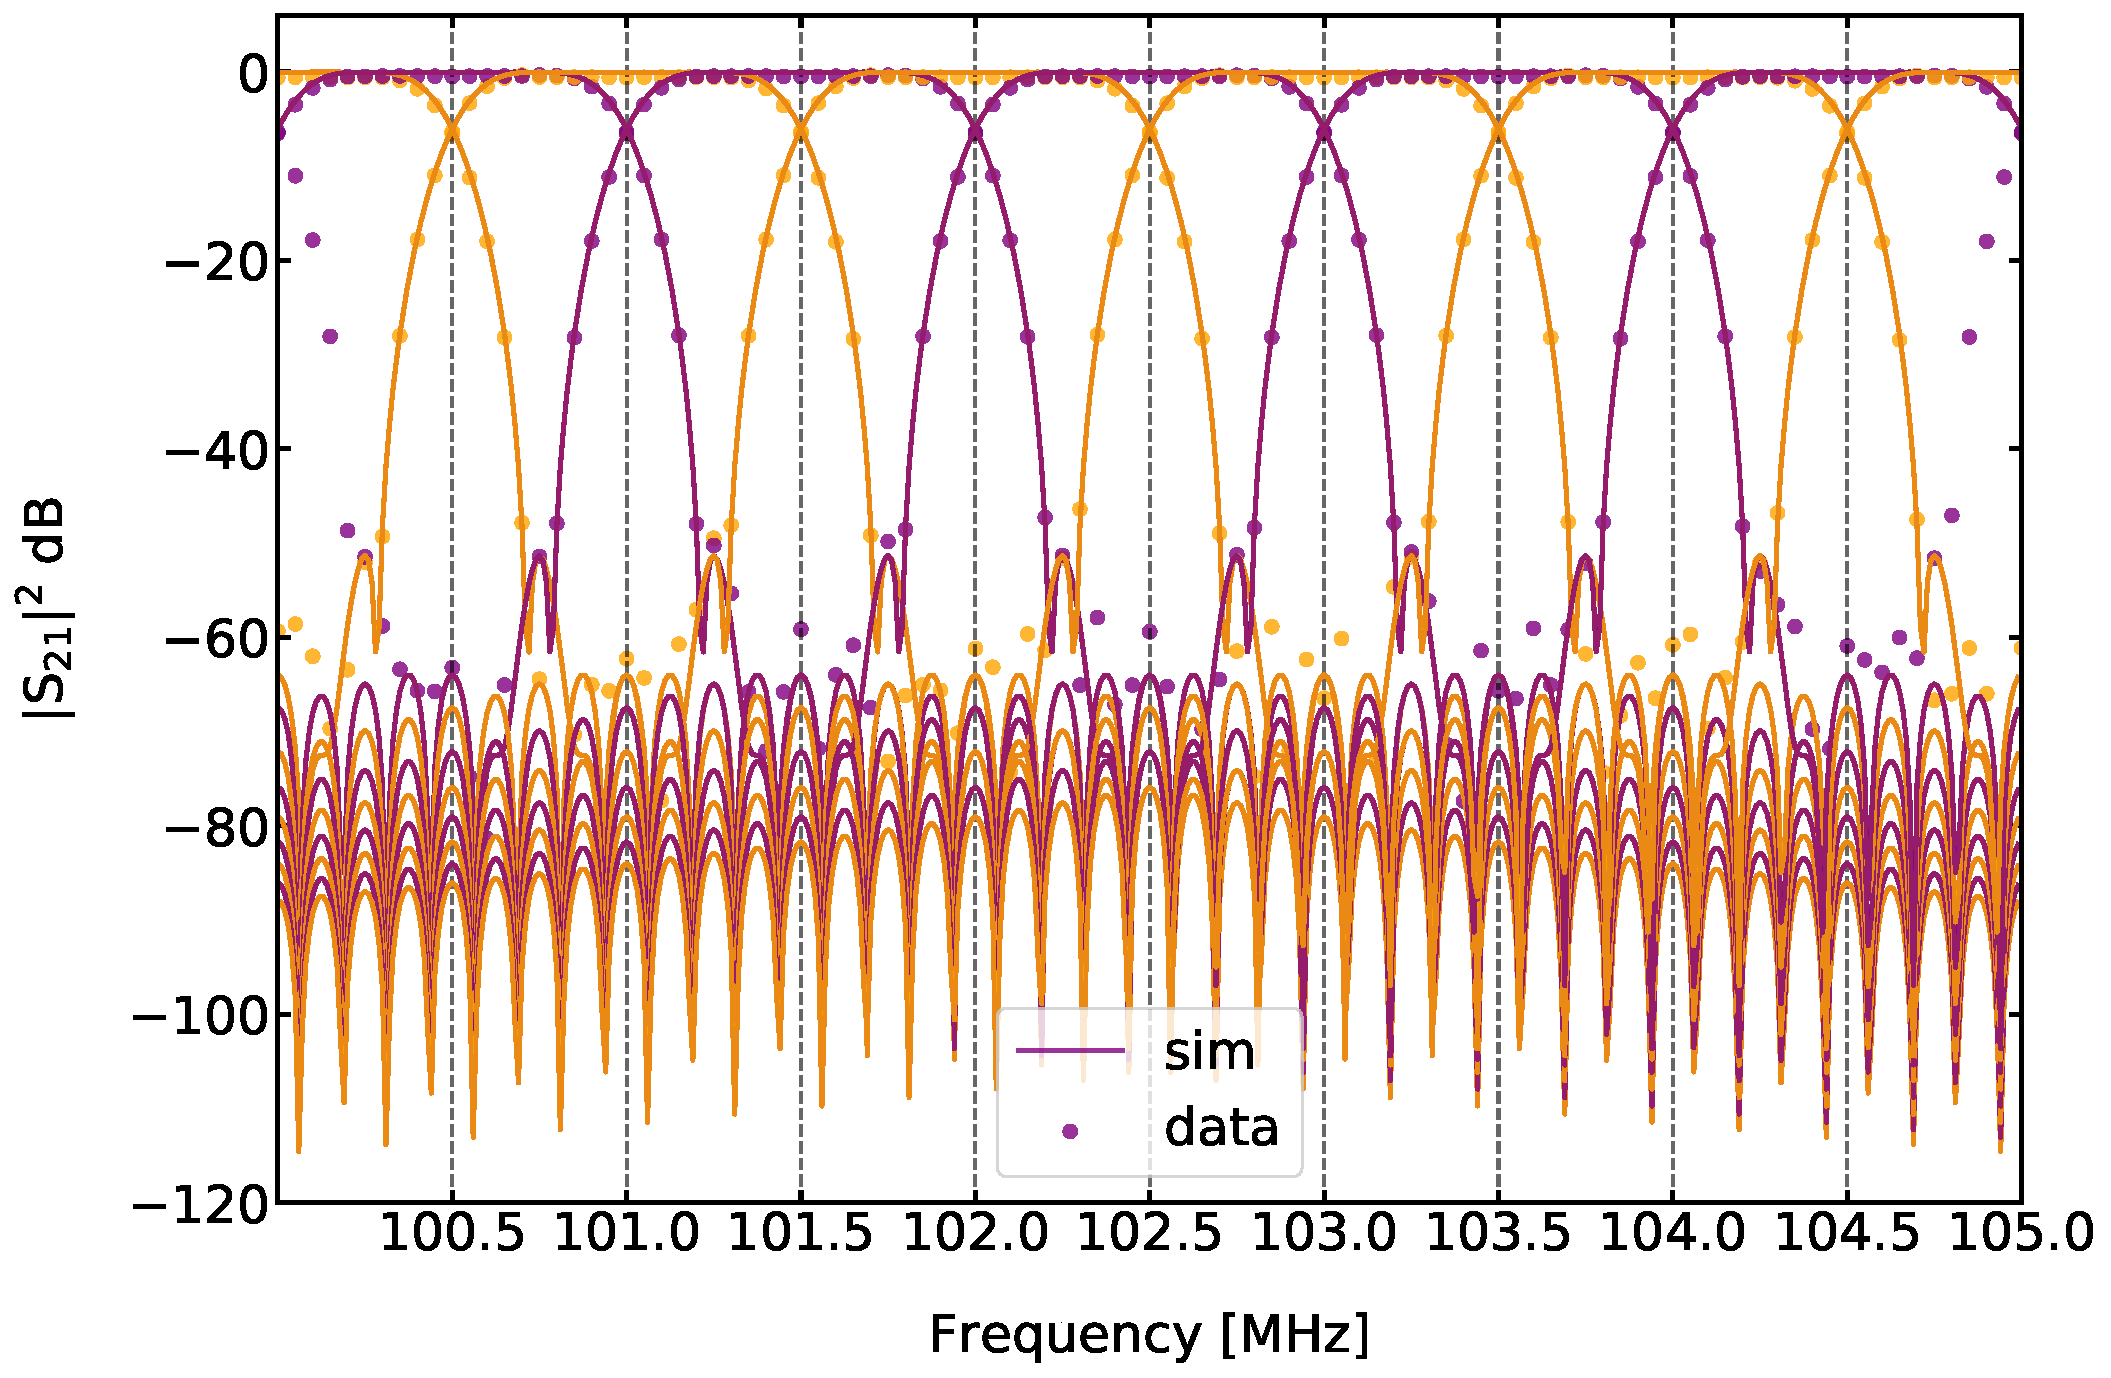
\includegraphics[width=\textwidth]{figures/readout/sim/pfb_fft_comp}
\caption[A 5~MHz section of the transfer function of the firmware PFB-FFT, showing measured (dots) and simulated values (lines).]{A 5~MHz section of the transfer function of the firmware PFB-FFT, showing measured (dots) and simulated values (lines). The PFB has widened the FFT bins so that they overlap at -6~dB. Their FHWM width is 450~kHz.}
\label{fig:pfb fft zoom}
\end{figure}

\subsection{FFT Bin Selection}\label{bin select}

When the LEKID resonant frequencies are irregularly spaced (as is the case for the BLAST-TNG arrays), some PFB-FFT bins contain multiple probe tones, while others remain empty (containing only noise). Only the former set of bins requires further channelization. The channel selection logic requires that up to 1024 channels from the FFT bin stream be selected within 512 clock cycles. To manage this while continuously streaming data, a buffered switch is constructed using Xilinx dual-port BRAM blocks. During software synthesis of the $I/Q$ waveform buffers, a list of up to 1024 bins is pre-calculated based on known resonator frequencies and loaded into a dual-port `bin select' BRAM\@. The list may consist of any combination of the 1024 available bin indices, including a single bin index repeated 1024 times. If only a subset of bins is required, any unused RAM addresses are initialized to zero. Once the bin list is loaded into RAM, the bins are referred to as channels, with the channel order corresponding to the order of the original list. During operation, the bin indices for two consecutive channels are read out in parallel from the dual-port RAM\@. Each bin index is halved to represent the clock cycle (`clock address') corresponding to its offset in cycles from the zeroth FFT bin, and these clock addresses are to be used as read addresses for another dual-port RAM containing the bin data. In the data RAM, the contents of two consecutive bins are stored in each address slot.

In read mode, the contents of two bins are presented at each output port of the dual-port data RAM, the addresses of which are chosen by the clock addresses of the desired bin indices. Out of the four available bins to choose from on each cycle, only one member of each pair is desired. To determine which member of each bin pair to use, the least significant bit of the desired bin index is used to operate a switch that slices the proper bin from each pair. The new pair of bins is then passed through a MUX selector and sent to the first stage of the DDC\@. To facilitate continuous readout, the bin selector is duplicated into a read branch and a write branch, which together form a buffered switch.

The bins which are selected for further processing are hereafter referred to as channels.

\subsection{Fine Channelization: Digital Down Conversion}\label{ddc}

As was discussed in Section~\ref{tone comb} The PFB-FFT operates on the digitized ADC timestream once every 512 clock cycles, and therefore any probe tone waveforms that have a period longer than the filterbank length of 1024 samples will exhibit unwanted phase rotation over the course of several FFTs. This results in amplitude modulation of $\widetilde{I}$ and $\widetilde{Q}$, where the AM frequency $f_{k} - f_{\mathrm{pr}}$. One approach to circumventing this issue would be to use a longer FFT, with bins so narrow that each $f_{\mathrm{pr}}$ falls very near to a bin center. The MUSIC firmware employed this approach, with a $2^{16}$-point FFT, resulting in bin width of $\sim${7.5}~kHz (\citet{duan2010open}). However, this method relies on the LEKID frequency spacing being somewhat uniform. Instead, we use digital down conversion (DDC) to demodulate the residual AM\@. The technique, which was previously implemented in the ARCONS firmware \citep{mchugh2012readout}, has the advantage of using fewer FPGA resources then the long PFB-FFT approach.

To downconvert each channel, the $\widetilde{I}/\widetilde{Q}$ output timestreams from each FFT bin are multiplied with their corresponding $I_{\mathrm{DDC}}$/$Q_{\mathrm{DDC}}$ entries from the DDC LUT\@. With each clock cycle, two consecutive channels are operated on in parallel. A single cycle of the operation involves performing the calculation:

\begin{equation}
  (\widetilde{I} + j\widetilde{Q})(Q_{\mathrm{DDC}} + jI_{\mathrm{DDC}})
\end{equation}

where $\widetilde{I}/\widetilde{Q}$ are of data type 18.17, $I_{\mathrm{DDC}}/Q_{\mathrm{DDC}}$ are 16.15, and the resulting output $I/Q$ values are 19.17. During this process, FFT bins which contain multiple channels are downconverted once per channel. For successful down conversion to occur, each channel of the DDC LUT must be synchronized with its corresponding $\widetilde{I}/\widetilde{Q}$ timestream at the output of the FFT\@. Otherwies, on system start, the first channel arriving at the downconverter will be out of sync channel-wise with its corresponding DDC tone by some number of clock cycles between 0 and 512. This `DDC shift' is constant for a given bitstream file, but due to differences in how the System Generator places the logic during each compilation, the DDC shift varies by a small number of clock cycles between different bitstreams.

For each firmware file, the DDC shift can be discovered on system startup by using an algorithm built into the readout software (see Section~\ref{software}). The software steps through each possible DDC shift using the variable delay block while monitoring the snap block data from the DDC for a single channel. At each shift, a software FFT of $\widetilde{I}/\widetilde{Q}$ is compared to that of $I_{\mathrm{DDC}}/Q_{\mathrm{DDC}}$. When the delay has been set properly, the FFTs will match. Once the shift is known, it is programmed into the variable delay block using a software register, and the value is thereafter left unchanged.

As stated above, FFT bins which contain $N$ probe tones are downconverted $N$ times. Each of the $N$ channels which result from this process contain the both the downconverted probe tone, centered at DC, as well as non-zero signal contributions from the other probe tones which were present in the FFT bin prior to downconversion. These adjacent tones must be filtered out. Two methods were explored in order to achieve this. The first method is to add a low-pass FIR filter after the DDC, which is narrow enough to filter out any adjacent tones. The second method, which is what is used in the BLAST-TNG firmware, is to accumulate the $I/Q$ values for each channel (see Section~\ref{accum}). Accumulation both filters out the adjacent tones (it is a boxcar filter) and reduces the sample rate.

Relative to downsampling by accumulation, the FIR has the disadvantage of requiring many FPGA resources (delays, adders and multipliers). Because the $I/Q$ samples at the output of the DDC are time-multiplexed (equivalently, channel-multiplexed) ($I_{\mathrm{chan0}}/Q_{\mathrm{chan0}}$, $I_{\mathrm{chan1}}/Q_{\mathrm{chan1}}$, \ldots, $I_{\mathrm{chanN}}/Q_{\mathrm{chanN}}$) the FIR must also act in a time-multiplexed fashion. At the output of the DDC, the samples of any given channel appear once every 512 clock cycles. Therefore, the FIR must include a matching latency of 512 clock cycles between every addition. Following \citet{strader2016digitial}, the $n$th $I$ value to appear at the output of the FIR is therefore:

\begin{equation}
  I_{\mathrm{out}}[n] = \sum _{m=0}^{M - 1} h[m]I_{\mathrm{in}}[n - 512m]
\end{equation}

where $m$ is the channel index and $h$ is a filter coefficient. The filter coefficients are calculated in software, using a Hamming or Hanning window, and then programmed into software registers by the user. During system operation they can be reprogrammed at any time.

The need for long latencies make it difficult for System Generator to meet the design's timing constraints during the placement and routing stage of firmware compilation. In addition, to narrow the signal bandwidth from 500~kHz to $\sim$1~kHz requires the use of many filter taps ($\mathcal{O}(100))$. By simply co-adding (accumulating) consecutive samples from each channel, both filtering and downsampling can be achieved simultaneously, with less resource utilization. Ultimately, this was the option that was taken for the BLAST-TNG firmware.

Figure~\ref{fig:ddc1} and~\ref{fig:ddc1000} show frequency domain examples of the downconversion process for one channel from a tone comb consisting of one and 1,000 tones. In both figures, the top frame shows the input signal to the DDC, $X = \sqrt{\widetilde{I}^{2} + \widetilde{Q}^{2}}$, the middle frame shows the DDC tone $X_{\mathrm{DDC}}$, and the bottom frame shows the downconverted output signal $Y$. The spurs which are visible at either side of the central tone are due to the effects of quantization errors in the software FFT\@. In the channel from the multitone comb shown in Figure~\ref{fig:ddc1000}, the group of spurs centered at -50~kHz relative to the main tone is due to sideband leakage in the IF modulator. The sideband tones are down $\sim$-20 dB relative to the main tone's peak, and are averaged out during the accumulation stage.

\begin{figure}[!htbp]
\centering
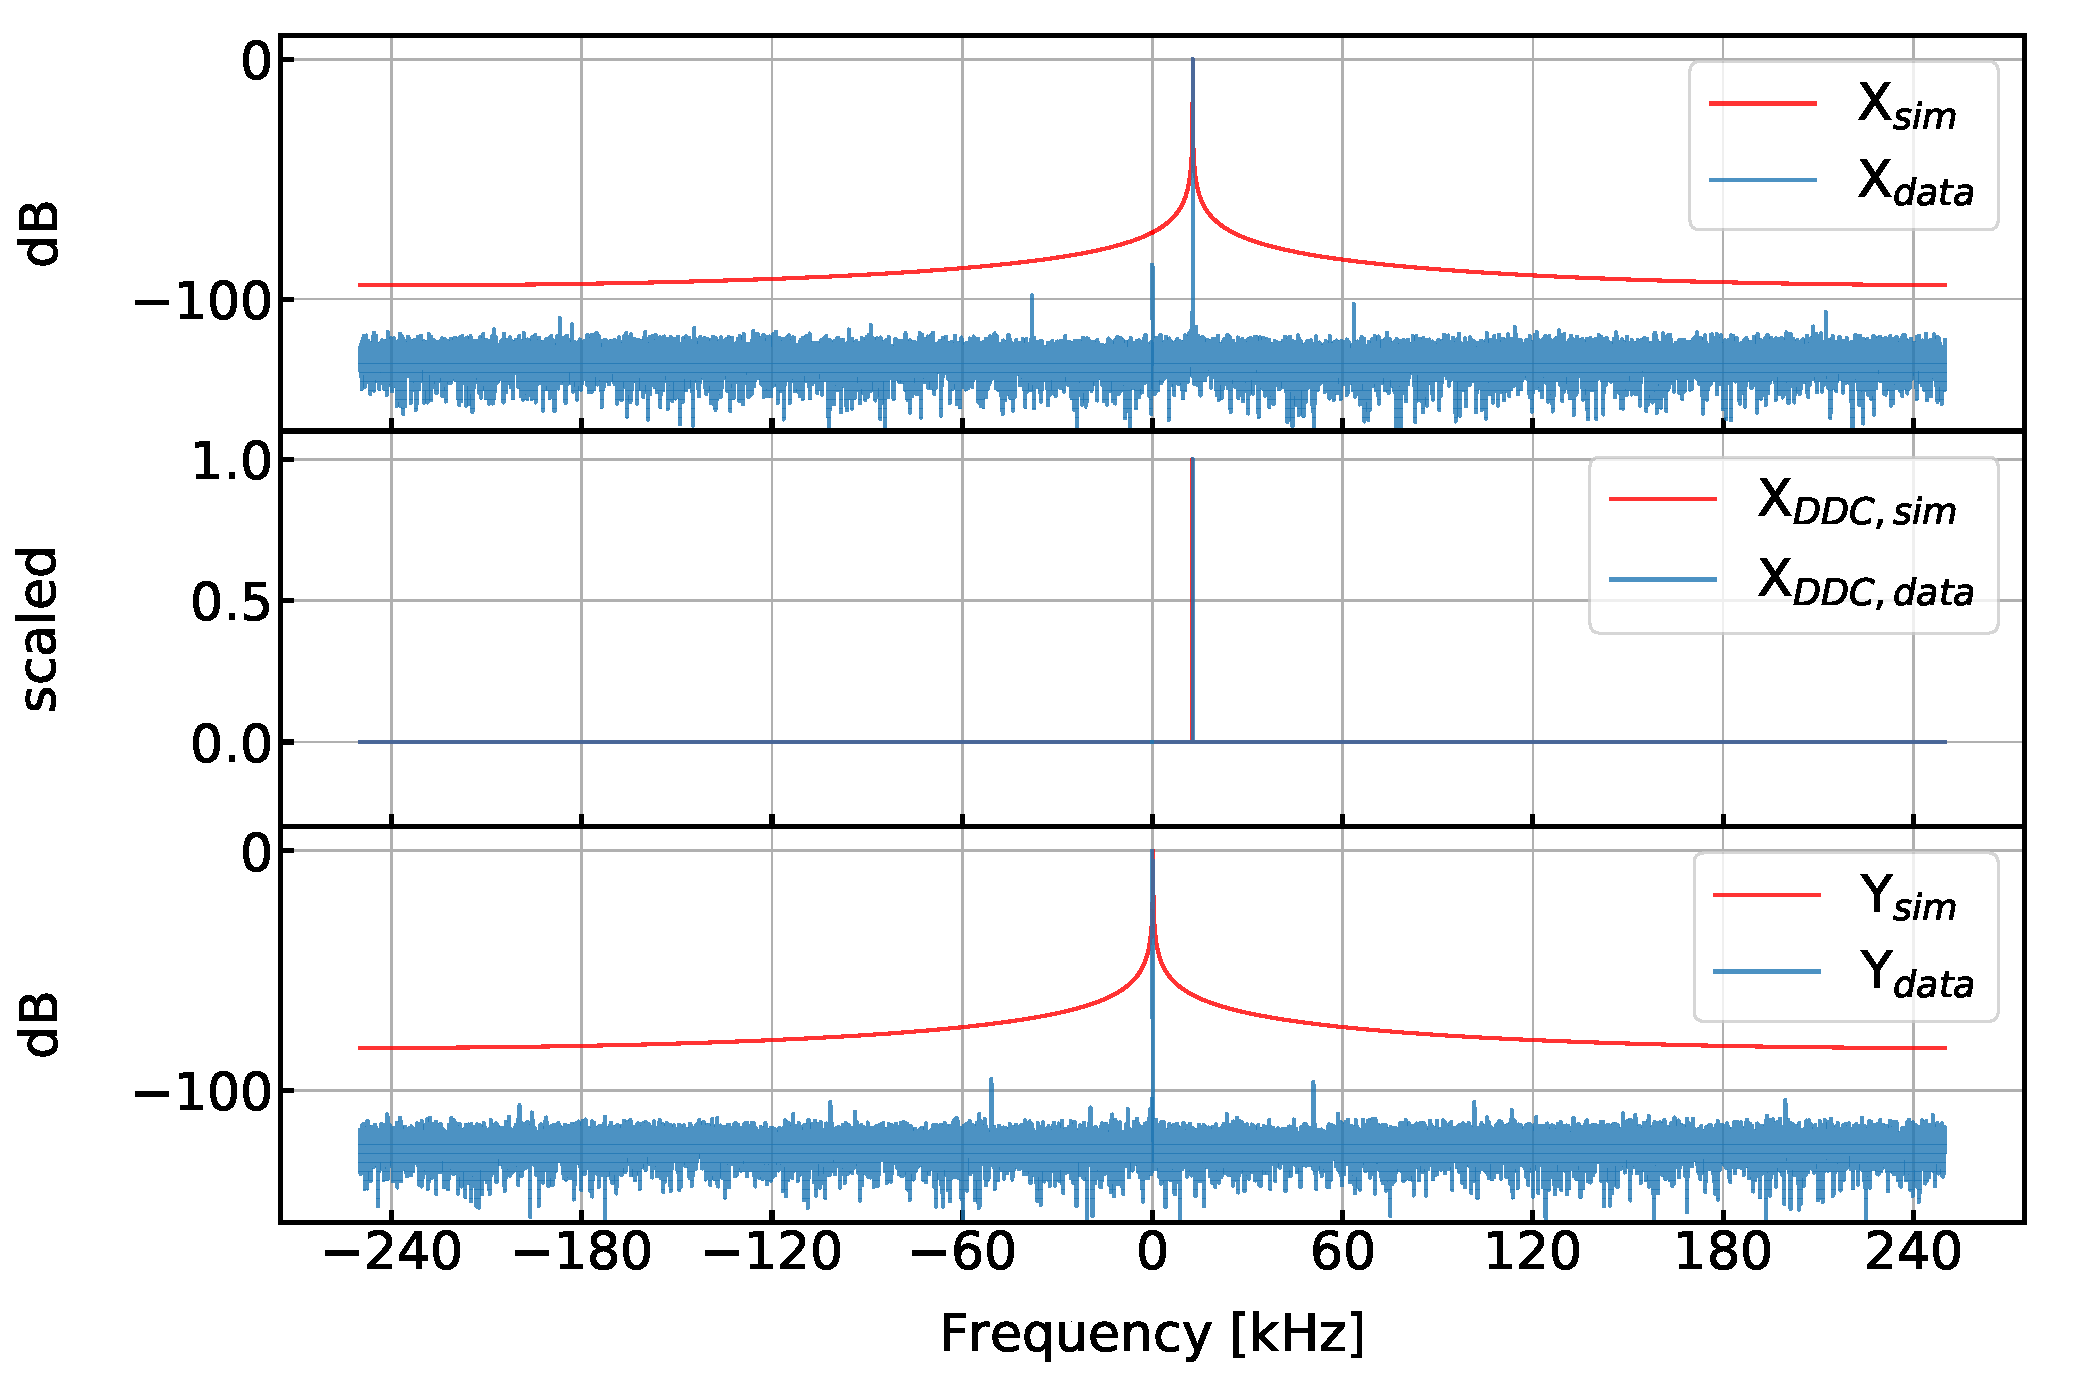
\includegraphics[width=\textwidth]{figures/readout/sim/ddc_sim_0}
\caption[An example of the frequency domain DDC products (measured and simulated) for one channel of a tone comb consisting of a single tone.]{An example of the frequency domain DDC products (measured and simulated) for one channel of a tone comb consisting of a single tone.}
\label{fig:ddc1}
\end{figure}

\begin{figure}[!htbp]
\centering
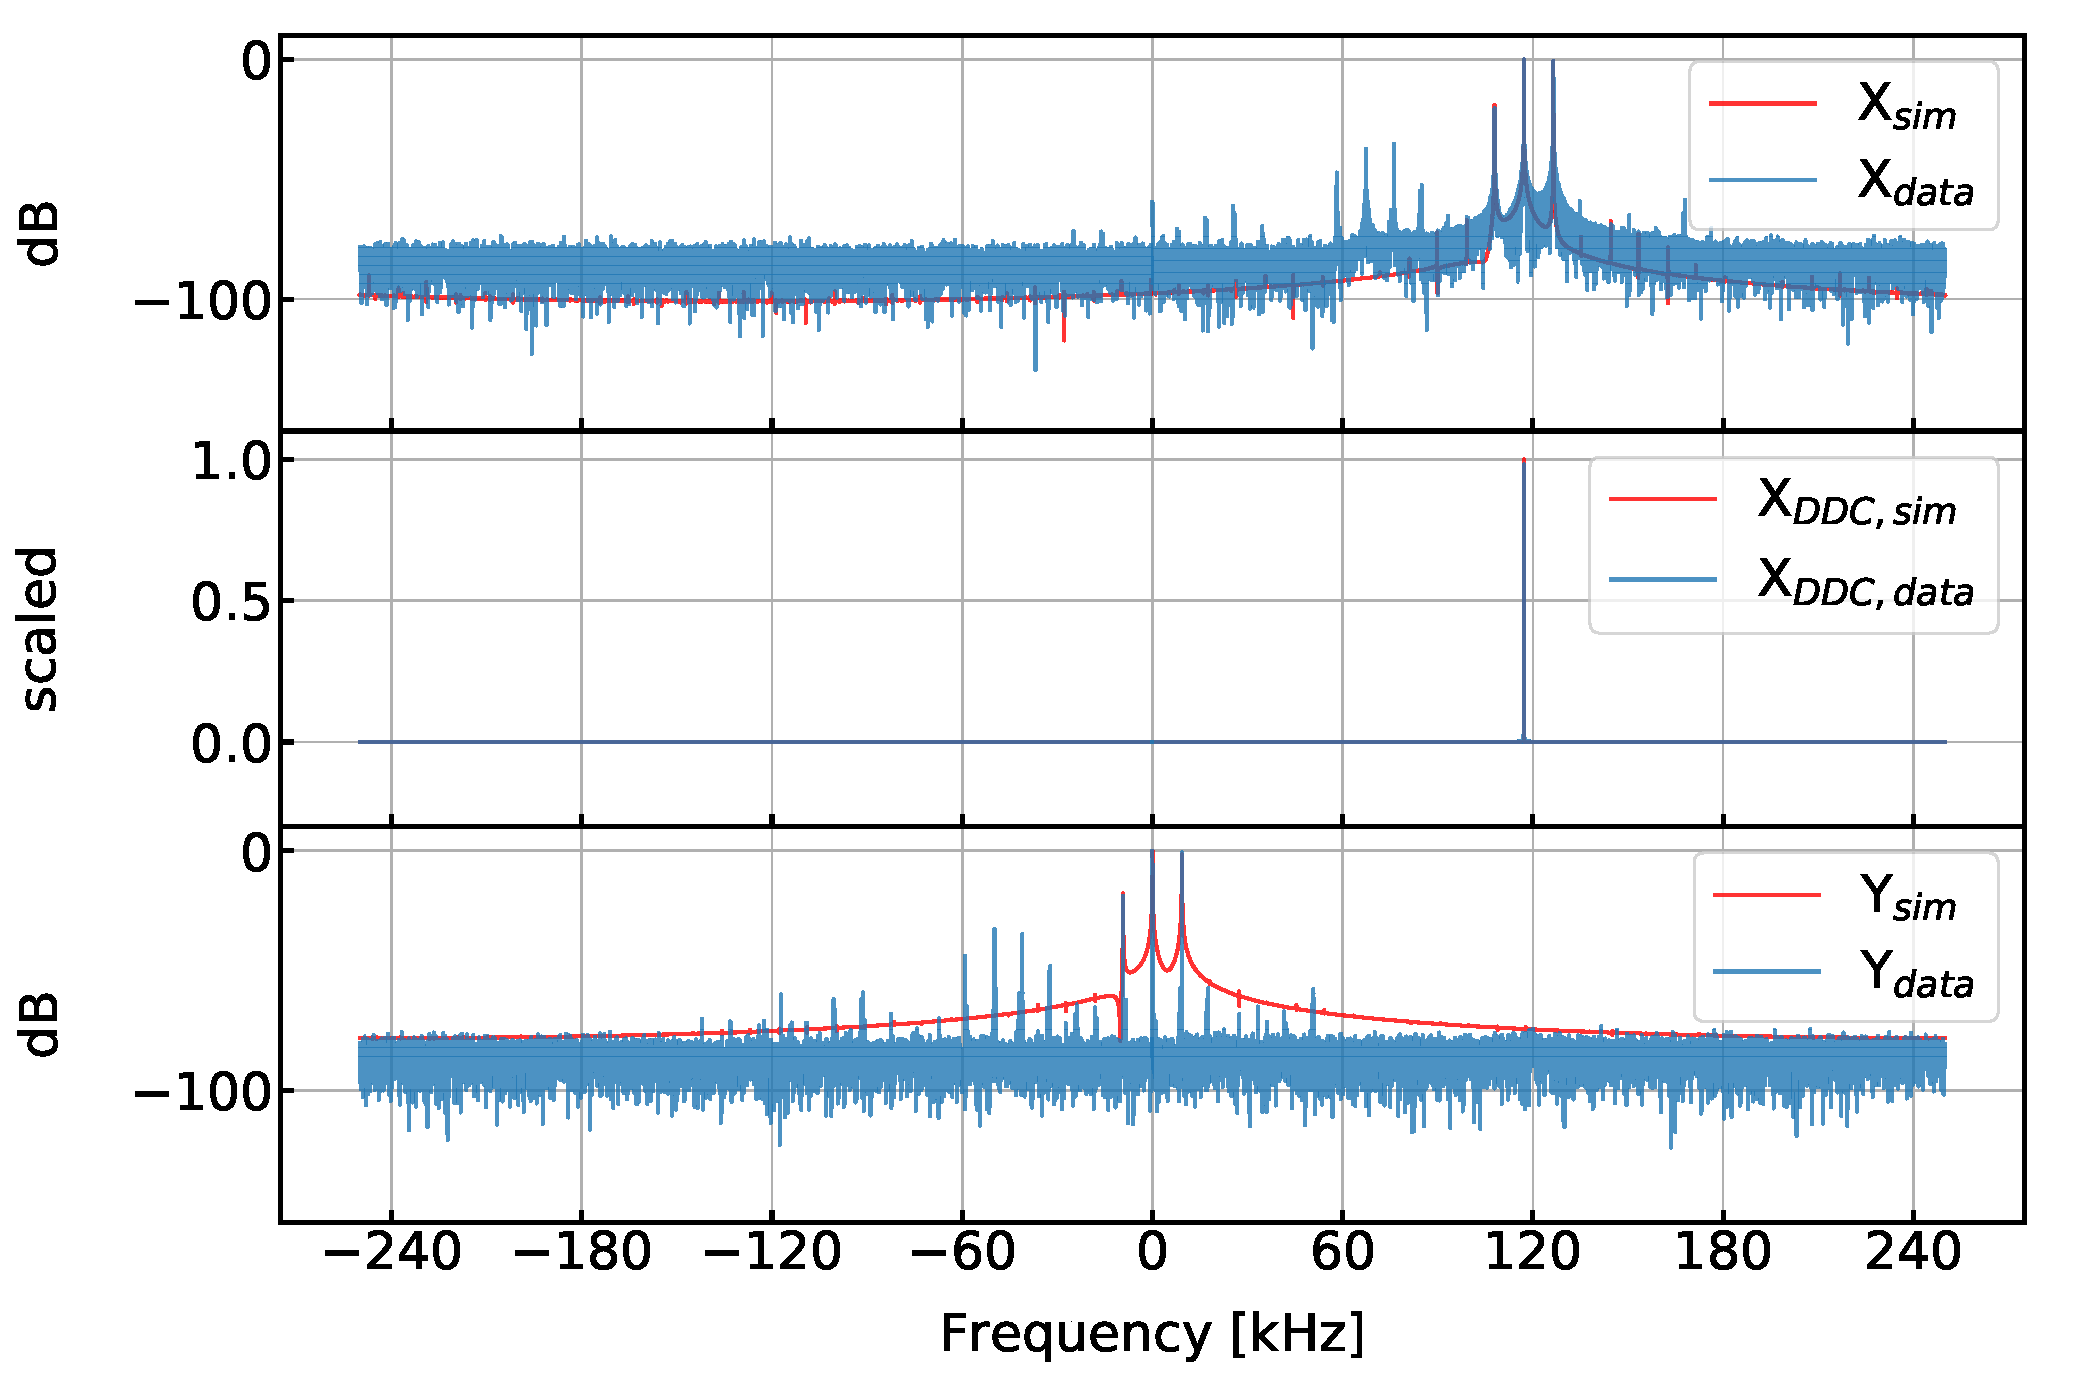
\includegraphics[width=\textwidth]{figures/readout/sim/ddc_sim_100}
\caption[An example of the frequency domain DDC products (measured and simulated) for one channel of a tone comb consisting of 1,000 tones.]{The frequency domain DDC products for one channel of a tone comb consisting of 1,000 probe tones, with measured (blue) and simulated data (red).}
\label{fig:ddc1000}
\end{figure}

\begin{comment}
\begin{figure}[!htbp]
\centering
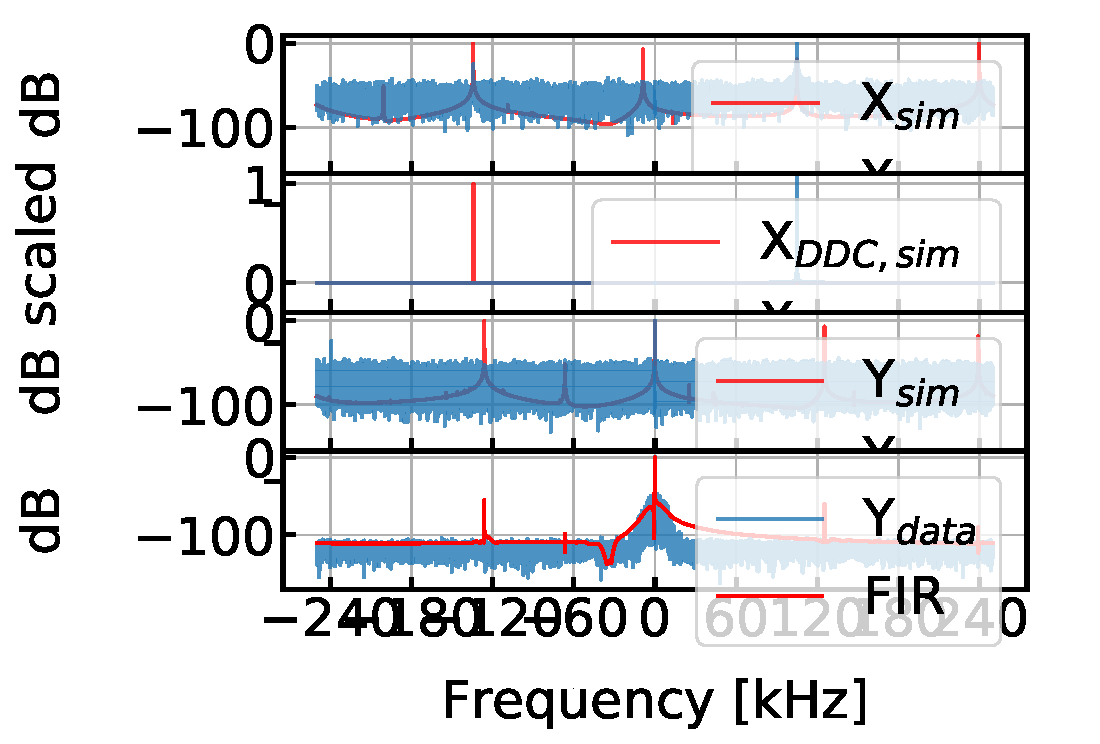
\includegraphics[width=\textwidth]{figures/readout/sim/ddc_sim_11}
\caption[An example of the frequency domain DDC products (measured and simulated) for one channel of a tone comb consisting of 628 tones, with the FIR applied to the DDC output.]{The frequency domain DDC products for one channel of a tone comb consisting of 628 probe tones, with measured (blue) and simulated data (red). An FIR has been applied to the DDC output timestream.}
\label{fig:ddcFIR}
\end{figure}
\end{comment}

\subsection{Accumulation and Downsampling}\label{accum}

The downconverter outputs $I/Q$ samples at a rate of $f_{\mathrm{DDC}} = 500$~kHz. The $I/Q$ timestreams at the output must be downsampled in order to output data at the desired rate. In the version of the firmware which does not contain the post-DDC FIR filter, the downconverted channels still contain signal from probe tones which were within the same PFB-FFT bin. While downsampling by decimation would require further filtering, downsampling by accumulation both decreases the data rate and filters out any signal which is non-periodic within the length of the accumulation.

Both downsampling and filtration are achieved by coherent channel-wise accumulation of the $I/Q$ values. The length of the accumulation is configured using a software register. The total number of accumulations used determines the bandwidth of the channels which are output by the system. For BLAST-TNG, the accumulation length is set to $2^{19}$ clock cycles, which corresponds to $N_{\mathrm{accum}} = 1024$. The resulting readout frequency $f_{\mathrm{ro}} = 488.2815$~Hz, and the channel bandwidth $B_{\mathrm{chan}} = f_{\mathrm{ro}}/2 = 244.14$~Hz. Because the number of accumulations can be adjusted by factors of 2, $f_{\mathrm{ro}}$ may be set to values of $\approx$~30, 61, 122, 244, 488 or 976~Hz. The firmware architecture does not support $f_{\mathrm{ro}} > 976$~Hz.

Accumulation is performed using CASPER vector accumulator blocks of length 512. During the additions, the $I/Q$ values are permitted to grow to 32-bits. The averaging function of the accumulator is effectively a box-car filter, which provides low-pass filtering of the channel timestreams. It is not necessary to complete the average with division by the total number of accumulations. Following accumulation, the channel values are sent to the packetization stage. Figure~\ref{fig:accum} shows the uncorrected transfer function (frequency response) for the 512~MHz readout band for a tone comb comprised of 1,000 evenly spaced channels (the `VNA' comb). The orange trace was measured in digital loopback. In digital loopback, the DAC output is filtered and then input directly into the ADC\@. The blue trace show the full RF loopback (containing all IF electronics). The ripples in the RF loopback trace are a product of the frequency response from each IF component. This transfer function can be corrected for using software, by calculating and applying the inverse transfer function for each readout slice (see Section~\ref{TRF}).

\begin{figure}[!htbp]
\centering
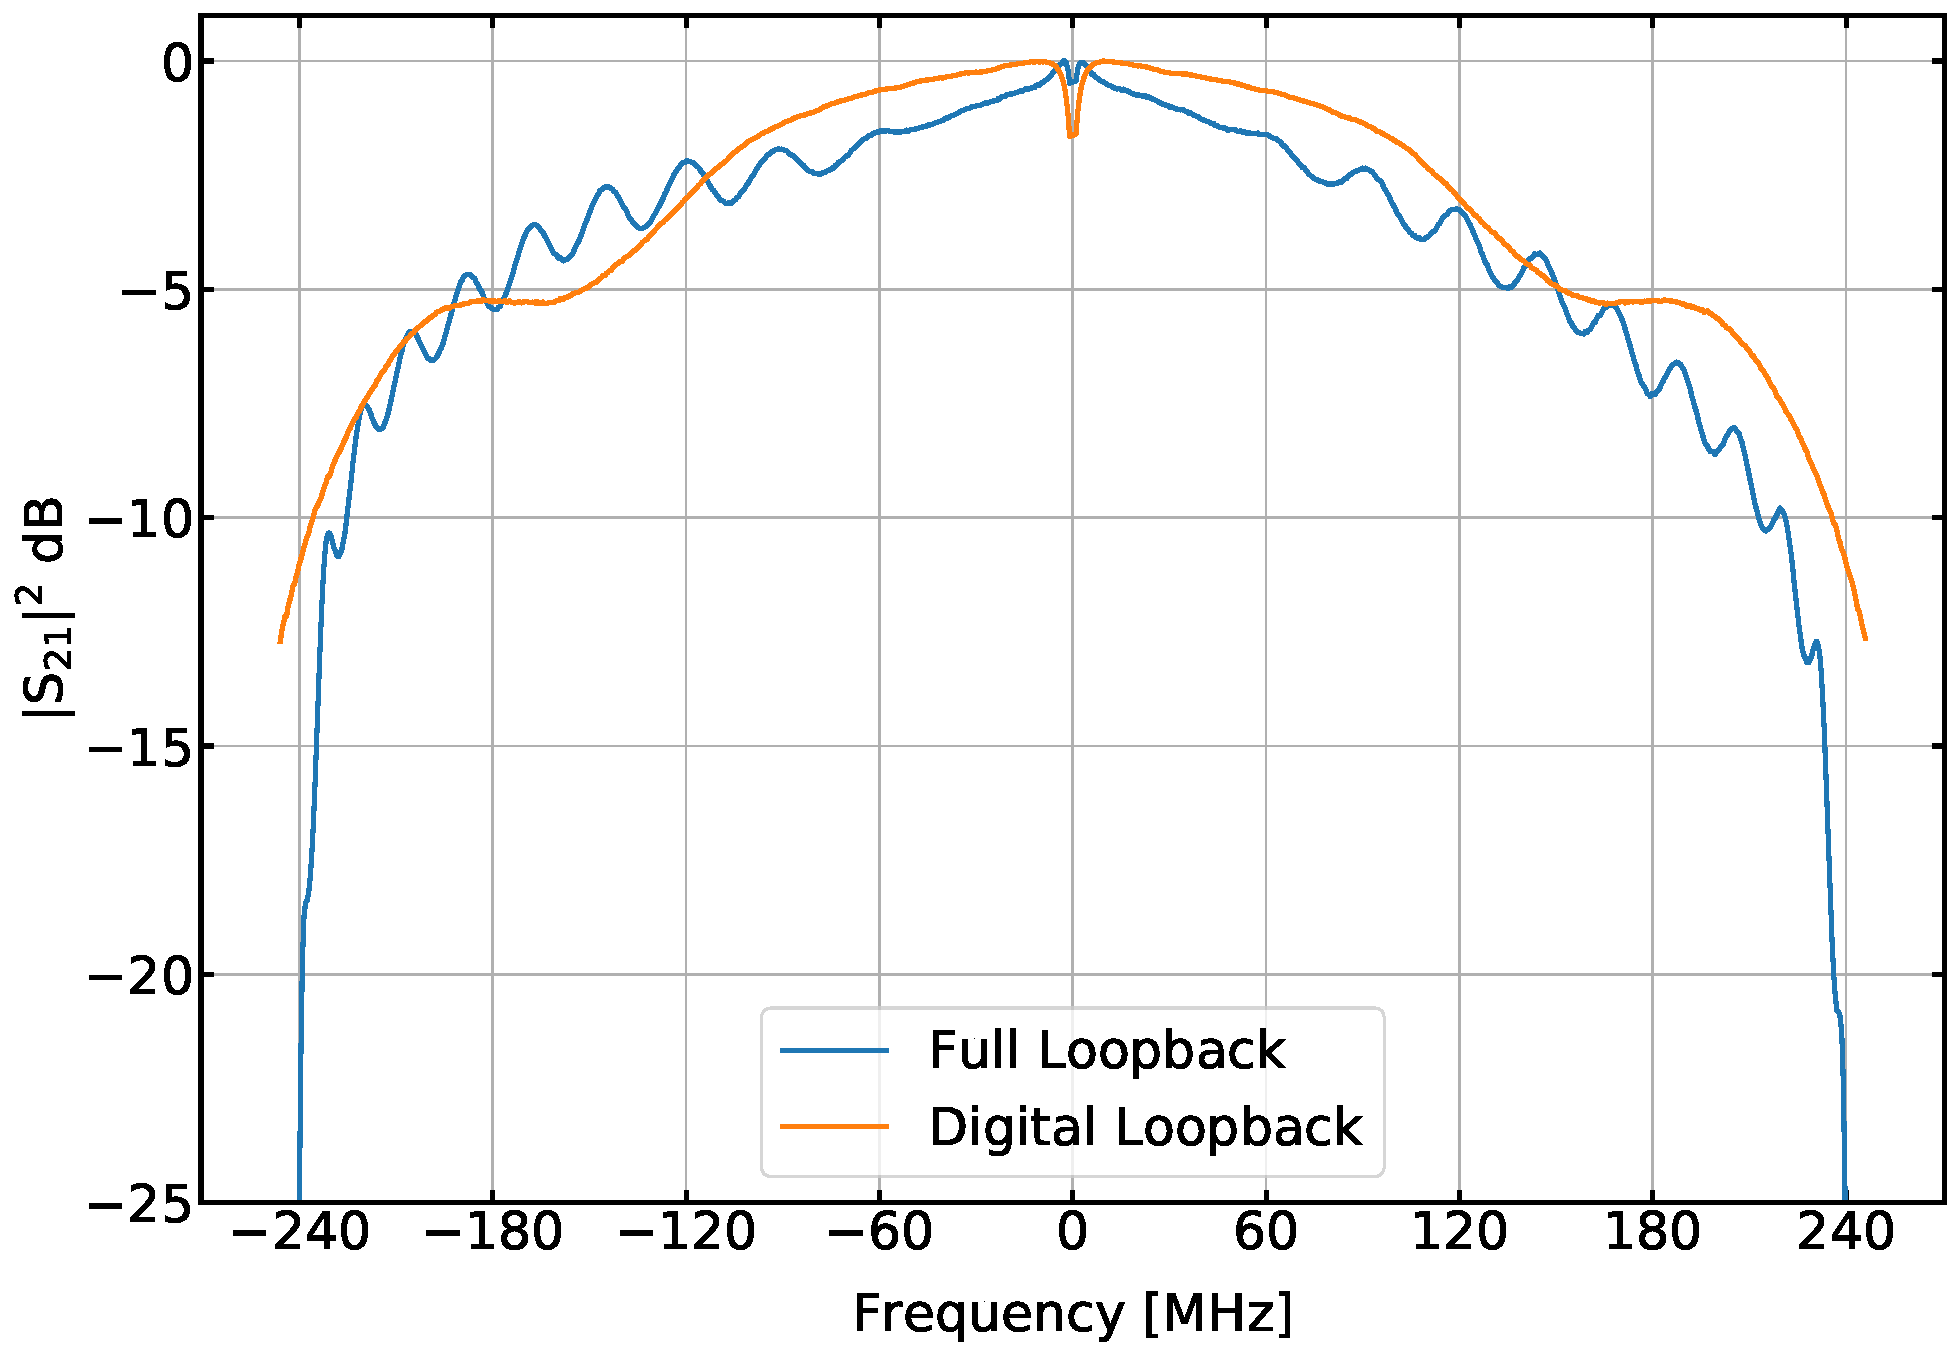
\includegraphics[width=\textwidth]{figures/readout/sim/accum_1000_lpf_nolpf}
\caption[The transfer function of the accumulator (\macrocapwrap{|S$_{21}$|$^{2}$}), for a tone comb consisting of 1,000 tones, in digital and RF loopback.]{The transfer function of the accumulator (|S$_{21}$|$^{2}$), for a tone comb consisting of 1,000 tones, in digital and RF loopback.}
\label{fig:accum}
\end{figure}

\subsubsection{UDP Packetization and Time Stamping}\label{packets}

UDP packetization is performed using the CASPER 1GbE block. Because the block accepts only one byte at a time, each 4-B $I$ or $Q$ word must be sliced byte-wise before being input to the block.

The data packet size is fixed at 8234-B, regardless of the number of channels which is used. Figure~\ref{fig:data packet} shows the structure of a single UDP frame. Each packet contains a 42-B header, and 8192-B of data, which includes the $I/Q$ values for each channel, as well as time stamp and checksum information. The UDP header contains the source and destination MAC addresses, IP addresses and UDP ports, where the source values correspond to the FPGA Ethernet device on the ROACH2 board, and the destination values correspond to the data acquisition computer (DAQ). Each of these parameters is chosen by the user and programmed into the firmware using software registers during system startup.

After the header, there are 8192-B allocated for data storage. The first 8218-B contain the $I/Q$ values, which are stored as signed, 4-B words in little-endian:

\begin{itemize}[nosep]
  \item Words 1--512: $I$, channels 0--512
  \item Words 513--1024: $I$, channels 0--512
  \item Words 1025--1536: $I$, channels 513--1024
  \item Words 1537--2032: $I$, channels 513--1016
\end{itemize}

\vspace{5mm}

The last 8 $Q$ slots are used to store timestamp values, which limits the maximum channel count to 1016. The final 64-B of each packet contain timetamp information, a data checksum, and a free 4-B slot which can contain extra diagnostic information chosen by the user. The timing information is contained in 4 separate words, which are:

\begin{itemize}[nosep]
  \item ctime: The absolute Linux time, taken from the flight computer, and truncated to~$\upmu$s precision.
  \item PPS count: The number of elapsed PPS pulses since the PPS reset register was toggled.
  \item clock count: The number FPGA clock cycles which have elapsed between PPS counts.
  \item packet count: The number of packets which have been generated since the PPS reset register was toggled.
\end{itemize}

\vspace{5mm}

As described in Section~\ref{timing}, the combination of these values allows for the acquistion time of each data packet to be sychronized with the other telescope subsystems (most crucially, the pointing system) to within the required precision of $\sim$1~ms.

\begin{figure}[!htbp]
\centering
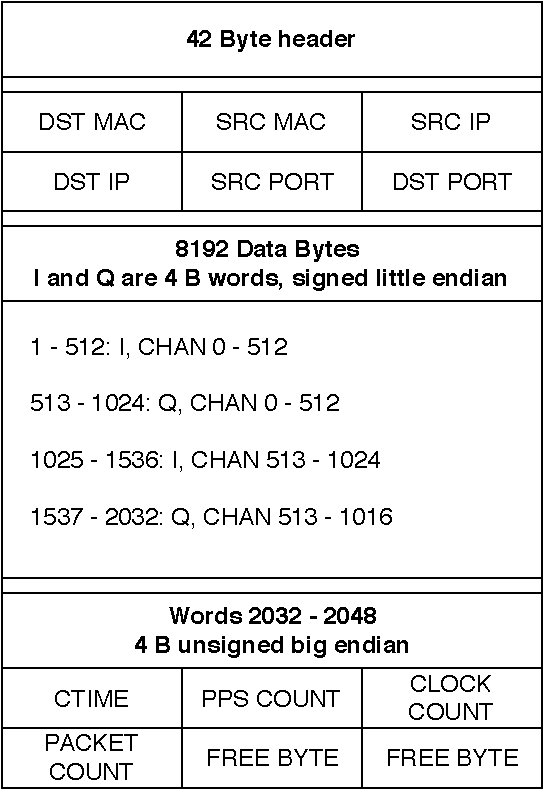
\includegraphics[scale=0.75]{figures/readout/schematics/roach_packet}
\caption[ROACH2 UDP packet structure.]{The structure of a ROACH2 UDP packet}
\label{fig:data packet}
\end{figure}

\section{Noise Verification}\label{noise verify}

In this section, we describe the verification of the WN and FN system requirements described in Sections~\ref{white noise} and~\ref{flicker noise}. To characterize these noise properties, we use the one-sided PSD, $S_{xx}(f)$:

\begin{equation}\label{eq:psd}
  S_{xx}[f]={\frac {1}{N f_{s}}}\left|\sum _{n=1}^{N}x_{n}e^{-j2\pi f n/f_{s}}\right|^{2}
\end{equation}

To obtain a better estimate of the PSD than Equation~\ref{eq:psd} can provide, we use the Welch Periodogram (WP) \citep{welch1967use}. The WP is an asymptotically unbiased estimator of the PSD\@. In Welch's method, a timestream is divided into $K$ windowed segments of equal length. The periodogram is calculated for each segment, and then averaged. The segments may also be overlapped in time. The variance of the WP is reduced by a factor of $1/K$ relative to a regular periodogram, at the expense of lower frequency resolution. The WP can be written as:

\begin{equation}\label{eq:WP}
S_{xx}[f] = \frac{1}{K} \sum_{n=0}^{K - 1}\frac{1}{f_{s} M} \left| \sum_{n=0}^{N - 1} x_{n,w} e^{-j2\pi f n / f_{s} }\right|^{2}
\end{equation}

where $x_{n,w}$ is a windowed version of the time series, and $M$ is the length of each segment. To fit the noise PSDs, we use a modified version of Leeson's equation, which empirically models the phase noise spectrum produced by a resonator \citep{lesson1966simple}. The model is a three-parameter fit to \gls{Sphase}:

\begin{equation}\label{eq:PSD fit}
  S_{\phi,fit}(f) = W\left[ 1 + \gls{fc}/f + \left( \frac{B_{\mathrm{res}}}{f} \right)^{2} (1 + \gls{fc}/f) \right] \qquad \left[  \frac{\mathrm{rad}^{2}}{\mathrm{Hz}} \right]
\end{equation}

where $W$ is the WN level, the resonator bandwidth $B_{\mathrm{res}} = (f_{0}/2\gls{Qr})$, and \gls{fc} the FN corner-frequency. The PSDs are measured in digital and RF loopack. In digital loopback, the MUSIC board DAC $I/Q$ outputs are passed through anti-aliasing filters and then fed directly into the ADCs. RF loopback includes the IF electronics. To simulate the gain of the BLAST-TNG cryostat, a 20~dB attenuator is placed between the RF out and RF in ports of the readout slice.

Figure~\ref{fig:psd 1000 fit} shows an example fit (red) using Equation~\ref{eq:PSD fit} to the median PSD of a tone comb containing 1,000 evenly spaced tones (blue), in digital loopback mode. In this particular example, the FN corner frequency $\gls{fc} \approx 0.5$~Hz, and the WN level is $\sim$-98~dBc/Hz.

\begin{figure}[!htbp]
\centering
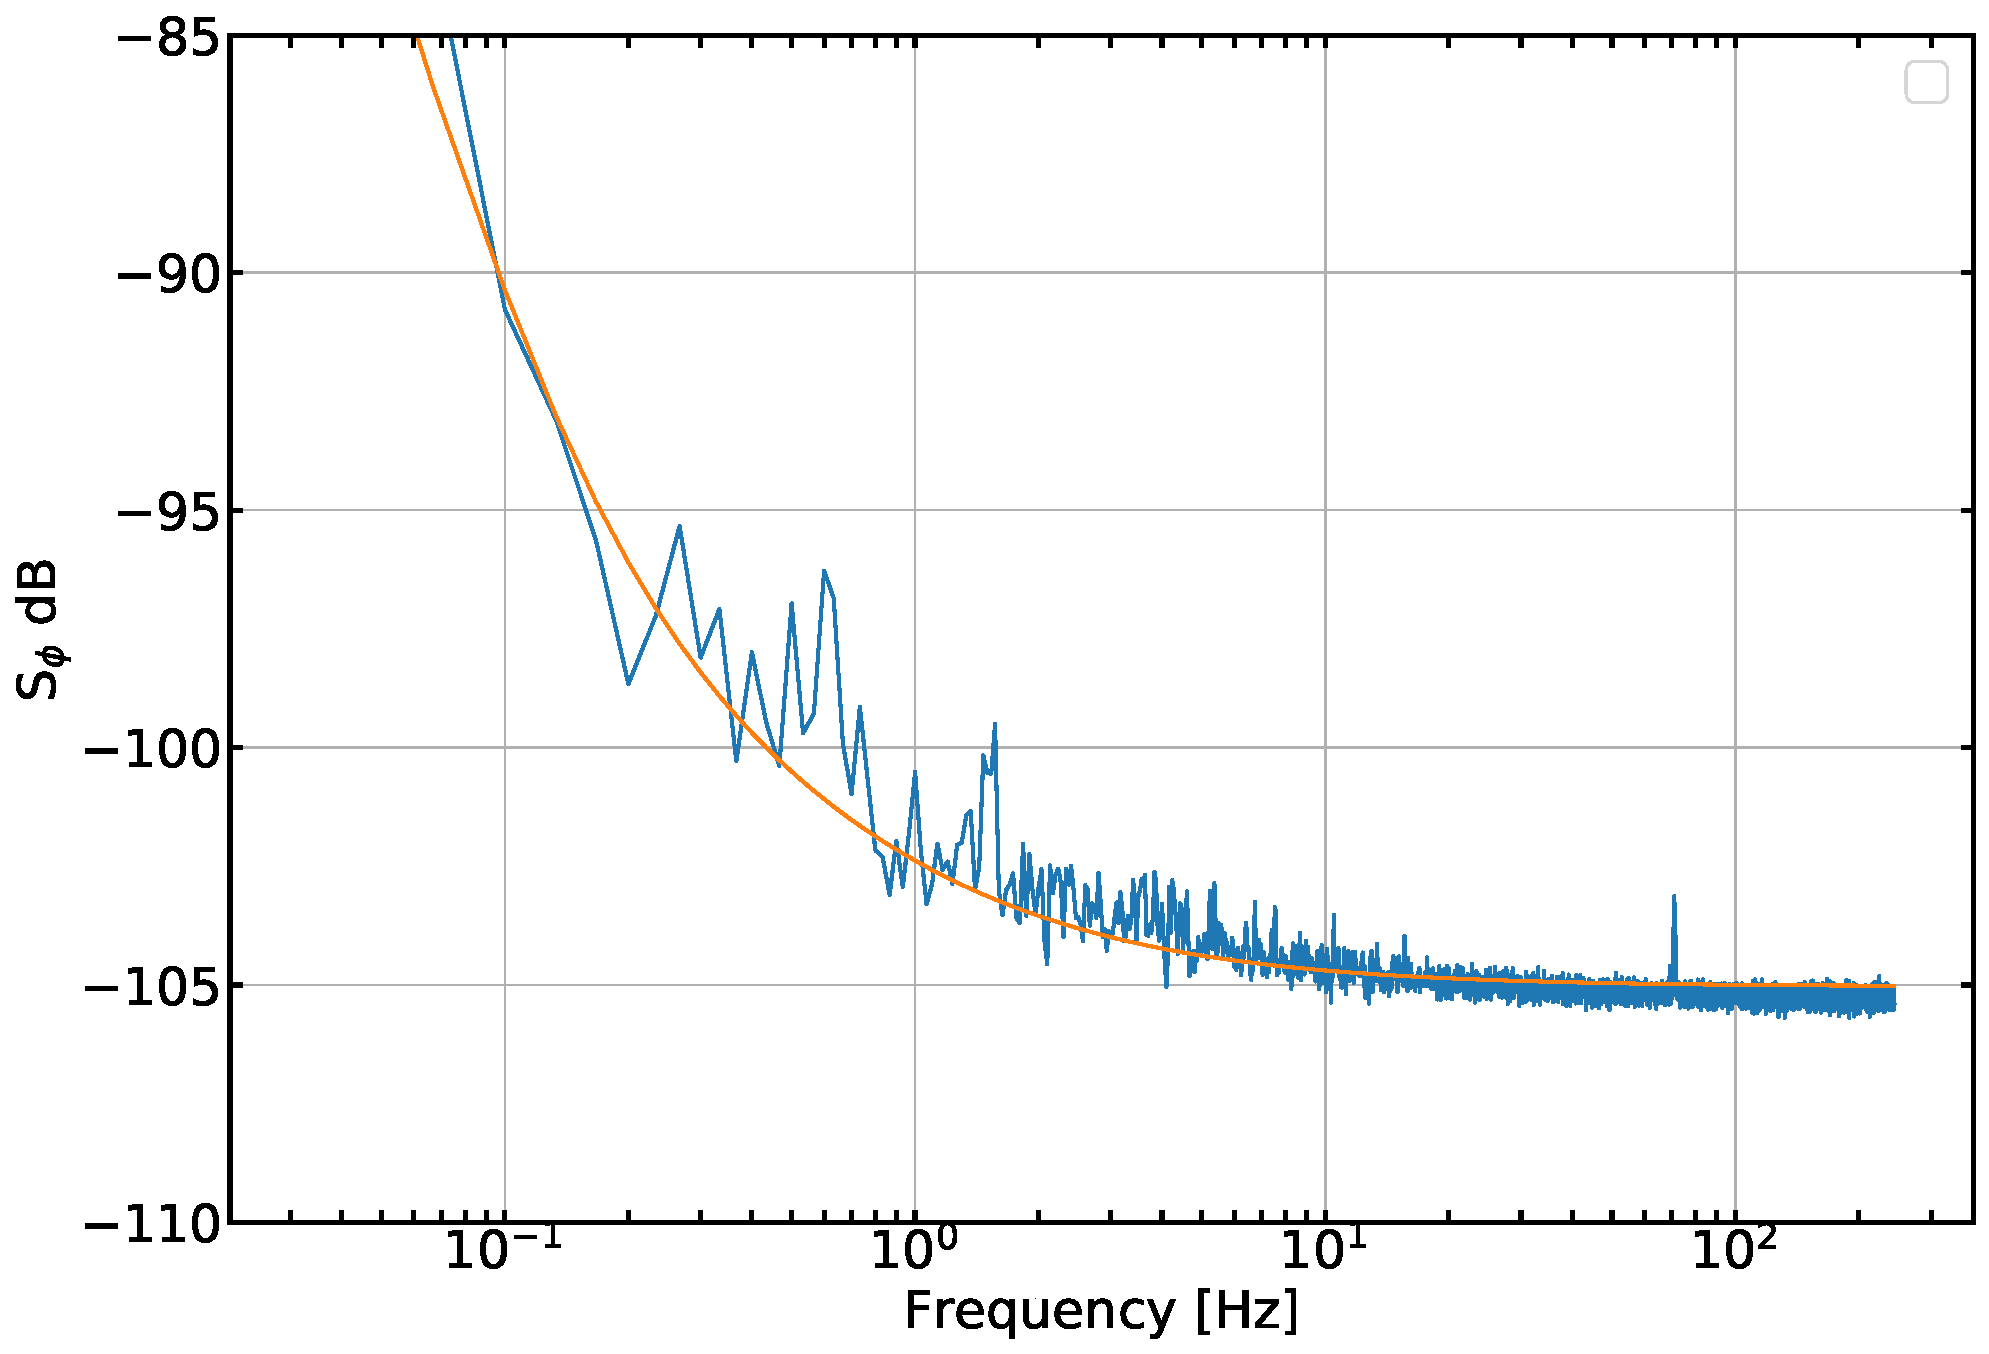
\includegraphics[width=\textwidth]{figures/readout/sim/c1000_PSD_fit}
\caption[A fit of a modified Leeson's equation to the median PSD for a tone comb containing 1,000 evenly spaced tones.]{A fit (red) of a modified Leeson's equation to the median PSD (blue) for a tone comb containing 1,000 evenly spaced tones.}
\label{fig:psd 1000 fit}
\end{figure}

In digital loopback mode, the noise was measured for tone combs containing 1, 100, 500, 618 and 1,000 tones. In the tone combs containing 100, 500 and 1,000 tones, the frequencies were evenly spaced by $\approx$~490~kHz. The tone comb with length 618 uses resonator frequencies which were identified for the 350~$\upmu$m array during detector testing at NASA's Columbia Scientific Balloon Facility in July, 2018 (618$_{350\mu m}$). These tones are not evenly spaced (see the discussion about detector yields in Chapter 4). The median PSDs calculated from each tone comb are shown in Figure~\ref{fig:dig loopback noise}. Table~\ref{tab:dig loopback} lists the WN level, in dBc/Hz and dB/Hz (converted using the method described in Section~\ref{white noise}, as well as the estimated CF, using Equation~\ref{eq:whitenoise}).

For the single tone comb, the WN level is measured to be $\approx$-143~dBc/Hz, which is within $\sim$1~dB of the theoretical minimum predicted by Equation~\ref{eq:whitenoise}. The WN levels for the evenly spaced tone combs are also close to their expected values. The 618$_{350\mu m}$ tone comb has a median WN level of $\approx$-105~dBc/Hz, which is close to the level measured for 1,000 evenly spaced tones. This small amount of excess noise is attributed to the uneven spacing of the probe tones, which creates intermodulation products in the analog modulator/demodulators. For each tone comb, the FN corner frequency is $\approx$0.5~Hz.

\begin{table}[!htbp]
\centering
\begin{tabular}{@{}llll@{}}
  \dtoprule{}
  N tones & S$_{\phi}$ (dBc/Hz) & S$_{\delta f / f}$ (dB/Hz) & Crest Factor est. (dB) \\ \midrule
  1 & -143 & -244 & 3 \\
  100 & -113 & -215 & 11 \\
  500 & -108 & -209 & 10 \\
  618$_{350\mu m}$ & -105 & -206 & 12.5 \\
  1000 & -105 & -206 & 10 \\ \dbottomrule{}
  \\
\end{tabular}
\caption[Digital loopback noise levels as a function of number of probe tones.]{The digital loopback WN levels as a function of 1, 100, 500, 618 and 1,000 tones. \macrocapwrap{618$_{350\mu m}$} is the tone comb for the 350~\macrocapwrap{$\upmu$m} band tones used during the 2018 Palestine instrument integration for BLAST-TNG\@. \macrocapwrap{\gls{Sff}} is calculated according to Equation \macrocapwrap{\ref{eq:Sff est}}, with \macrocapwrap{\gls{Qr} = 2.85 $\times$ 10$^{4}$}. The PSDs shown are the median of the PSDs calculated for each \macrocapwrap{$N$} value, from 60~s timestreams. \macrocapwrap{$CF$} is the estimated crest factor, in dB.}
\label{tab:dig loopback}
\end{table}

\begin{figure}[!htbp]
\centering
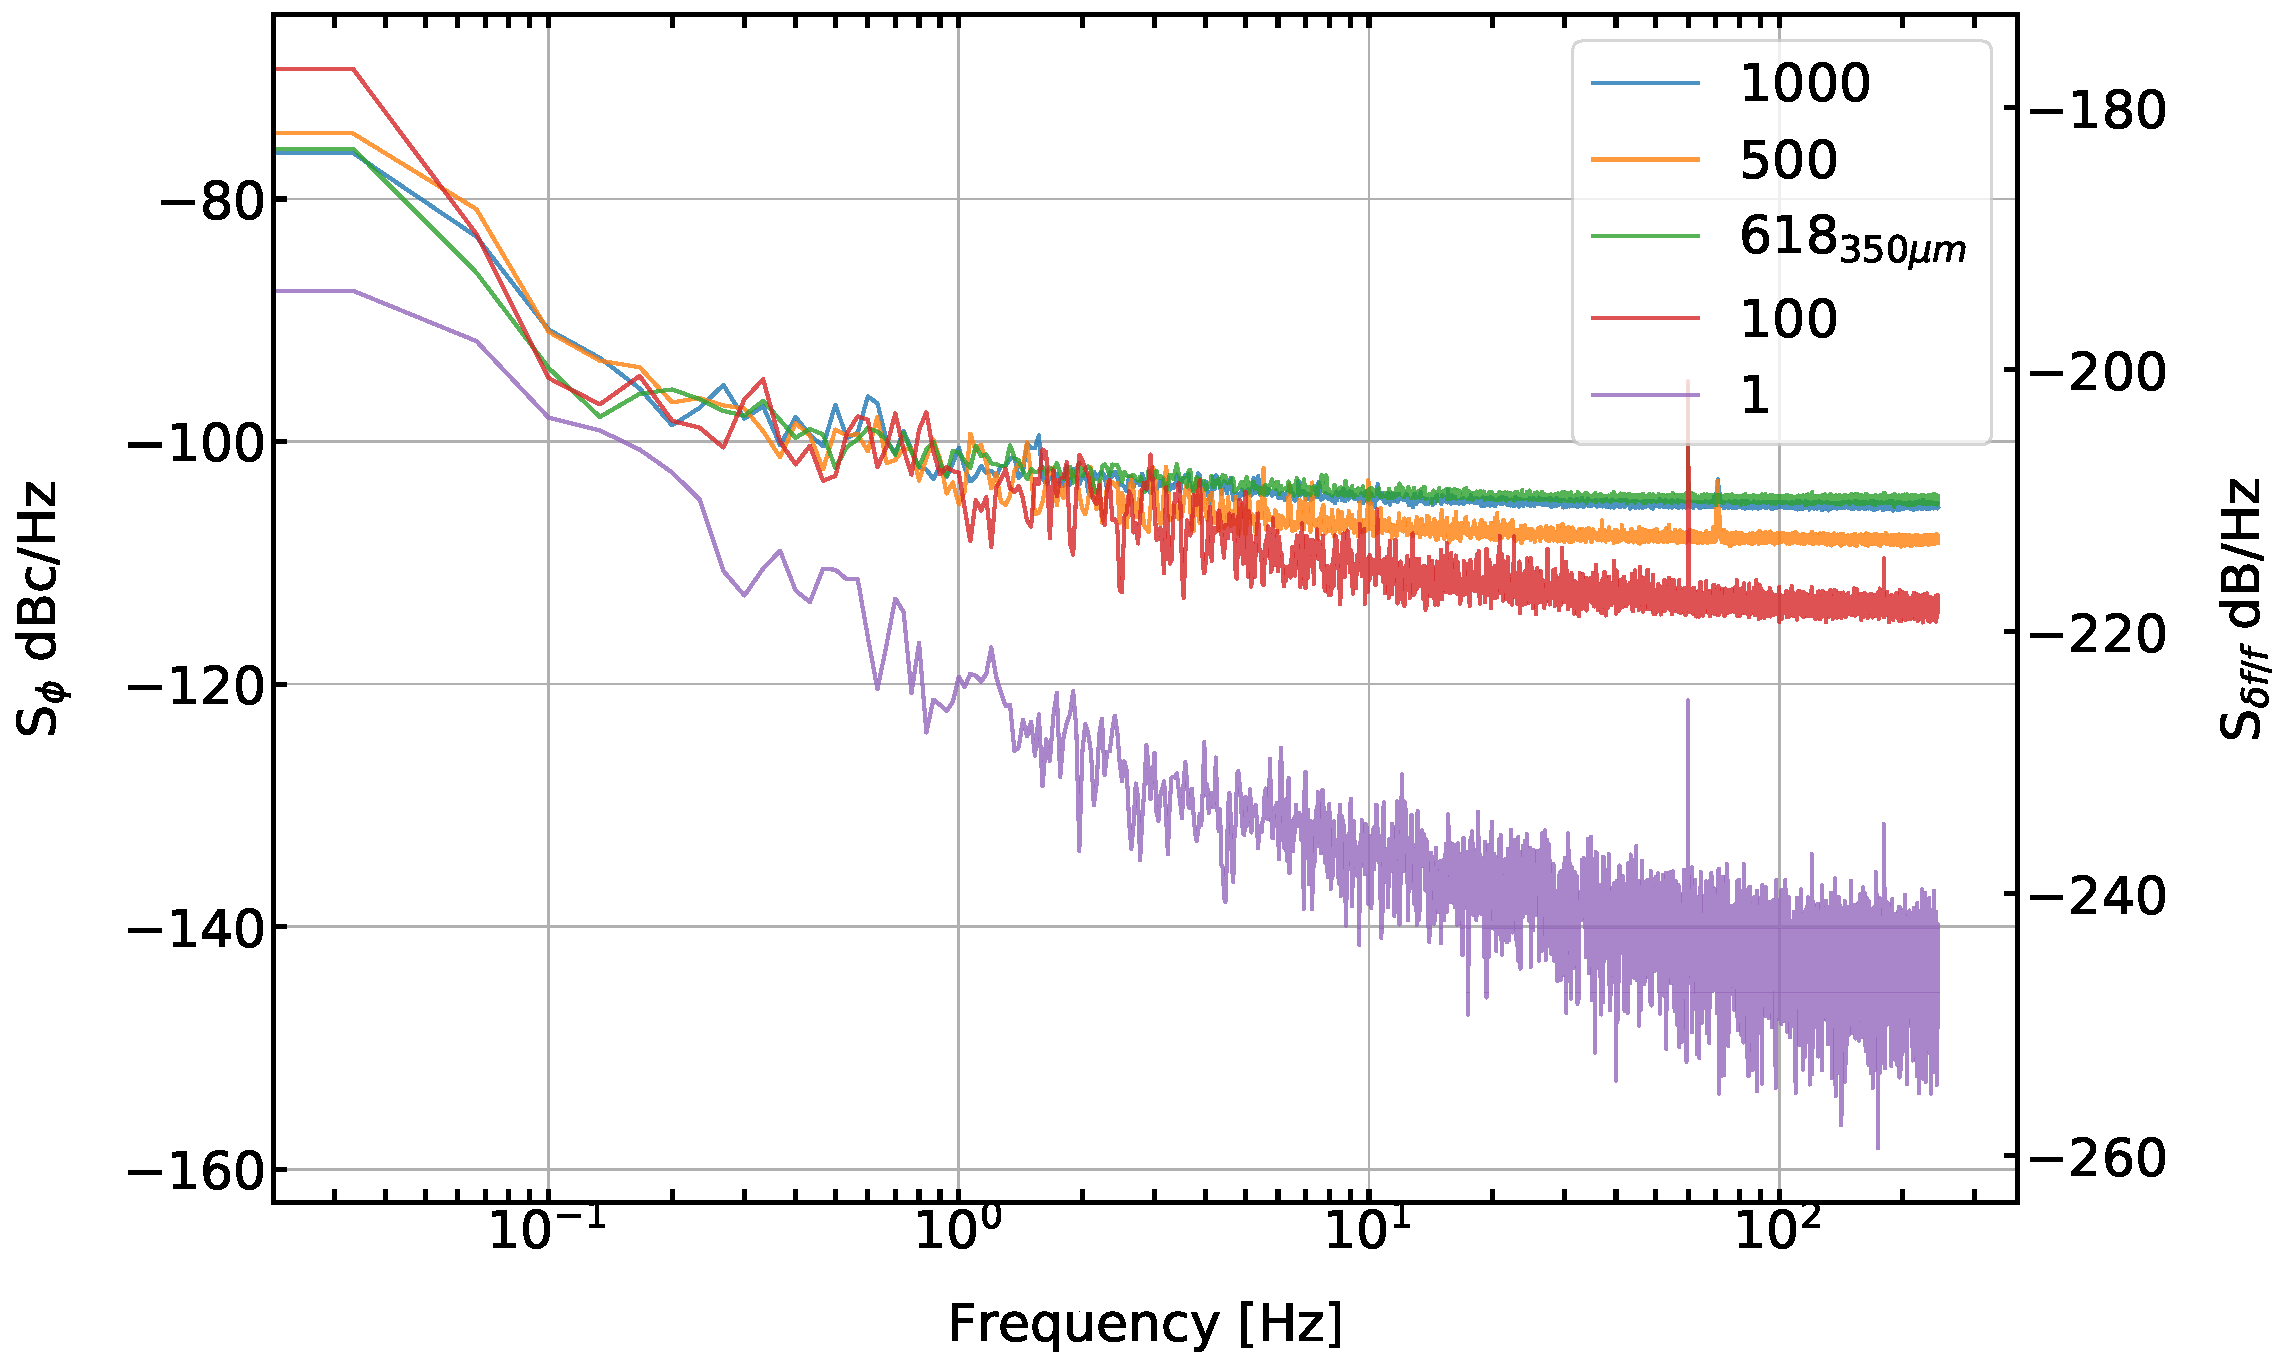
\includegraphics[width=\textwidth]{figures/readout/sim/LB_noise}
\caption[Digital loopback WN levels as a function of 1, 100, 500, 618 and 1,000 tones.]{The digital loopback WN levels as a function of 1, 100, 500, 618 and 1,000 tones. \macrocapwrap{618$_{350\mu m}$} is the tone comb for the 350~\macrocapwrap{$\upmu$m} band tones used during the 2018 Palestine instrument integration for BLAST-TNG\@. \macrocapwrap{\gls{Sff}} is calculated according to Equation \macrocapwrap{\ref{eq:Sff est}}, with \macrocapwrap{\gls{Qr} = 2.85 $\times$ 10$^{4}$}. The PSDs shown are the median of the PSDs calculated for each \macrocapwrap{$N$} value, from 60~s timestreams.}
\label{fig:dig loopback noise}
\end{figure}

The same median-PSD analysis was performed in RF loopback, using tone combs containing a single tone, the 618$_{350\mu m}$ tones and an evenly spaced comb of 1,000 tones (25 of which were removed from the data due to unusually high noise). The results of the analysis are shown in Figure~\ref{fig:rf loopback noise}. Table~\ref{tab:rf loopback} lists the WN levels as in Table~\ref{tab:dig loopback}, except the third column shows the estimated IF noise, in dB. The IF noise was estimated using Equation~\ref{eq:whitenoise} with the CF values in Table~\ref{tab:dig loopback}, and is found to be $\sim$5~dB in each measurement.

The WN level of the single tone is measured as -136~dBc/Hz, and those of the 1,000 and 618$_{350\mu m}$ combs are $\sim$~-98 dBc/Hz. These values are safely below the WN system requirement derived in Section~\ref{white noise}. However, the margin of error is only a few dB. As in digital loopback mode, the FN corner frequencies are $\approx$~0.5~Hz. While this value also satisfies the system requirement, there is little margin for error. It is therefore important to keep the noise contribution of the IF electronics as low as possible.

\begin{figure}[!htbp]
\centering
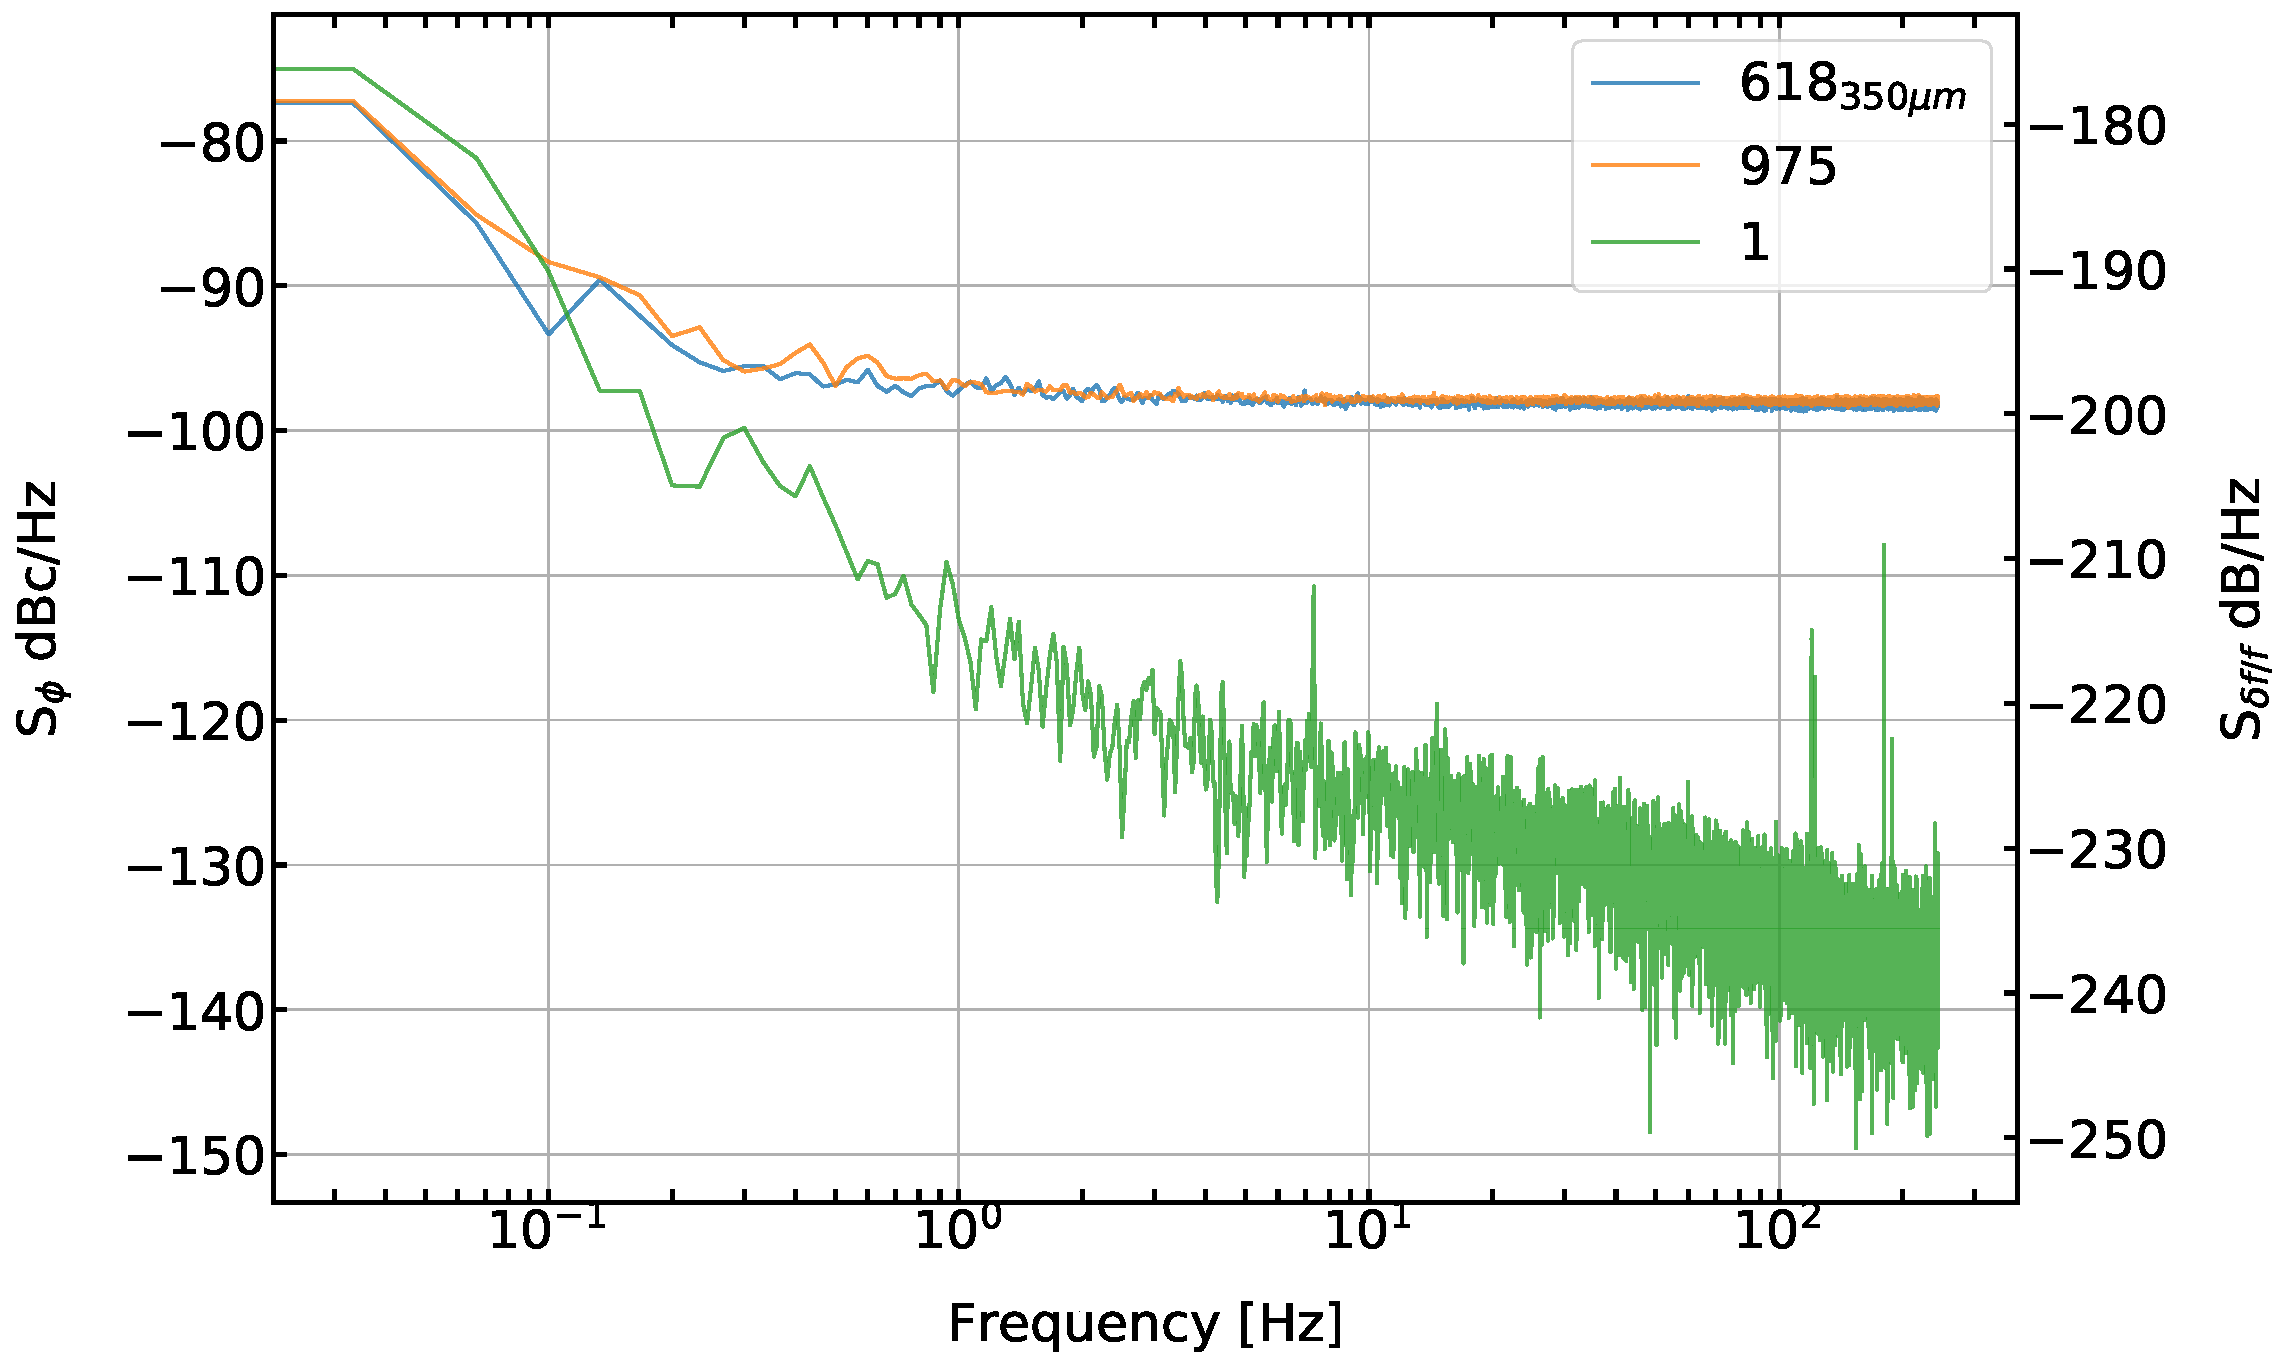
\includegraphics[width=\textwidth]{figures/readout/sim/IF_LB_noise}
\caption[The RF loopback WN levels as a function of 1, 618 and 975 tones.]{The RF loopback WN levels as a function of 1, 618 and 975 tones. 618$_{350\mu m}$ is the tone comb for the 350~$\upmu$m band tones used during the 2018 Palestine instrument integration for BLAST-TNG\@. \gls{Sff} is calculated according to Equation~\ref{eq:Sff est}, with\gls{Qr} = 2.85 $\times$ 10$^{4}$. The PSDs shown are the median of the PSDs calculated for each $N$ value, from 60~s timestreams.}
\label{fig:rf loopback noise}
\end{figure}

The WN and FN noise estimates presented in this section are in close agreement with those presented in \citet{gordon2016}, which have been measured using similar firmware and IF electronics.

\begin{table}[!htbp]
\centering
\begin{tabular}{@{}llll@{}}
\dtoprule{}
N tones & S$_{\phi}$ (dBc/Hz) & S$_{\delta f / f}$ (dB/Hz) & IF Noise (dB) \\ \midrule
1 & -136 & -237 & 4 \\
618$_{350\mu m}$ & -98 & -199 & 5 \\
1000 & -98 & -199 & 5.5 \\ \dbottomrule{}
\\
\end{tabular}
\caption[RF loopback noise levels for different numbers of probe tones.]{The RF loopback WN levels as a function of 1, 618 and 975 tones. 618$_{350\mu m}$ is the tone comb for the 350~$\upmu$m band tones used during the 2018 Palestine instrument integration for BLAST-TNG\@. \gls{Sff} is calculated according to Equation~\ref{eq:Sff est}, with \gls{Qr} = 2.85 $\times$ 10$^{4}$. The PSDs shown are the median of the PSDs calculated for each $N$ value, from 60~s timestreams. The last column is the estimated IF noise, in dB.}
\label{tab:rf loopback}
\end{table}

\begin{comment}
\begin{figure}[!htbp]
\centering
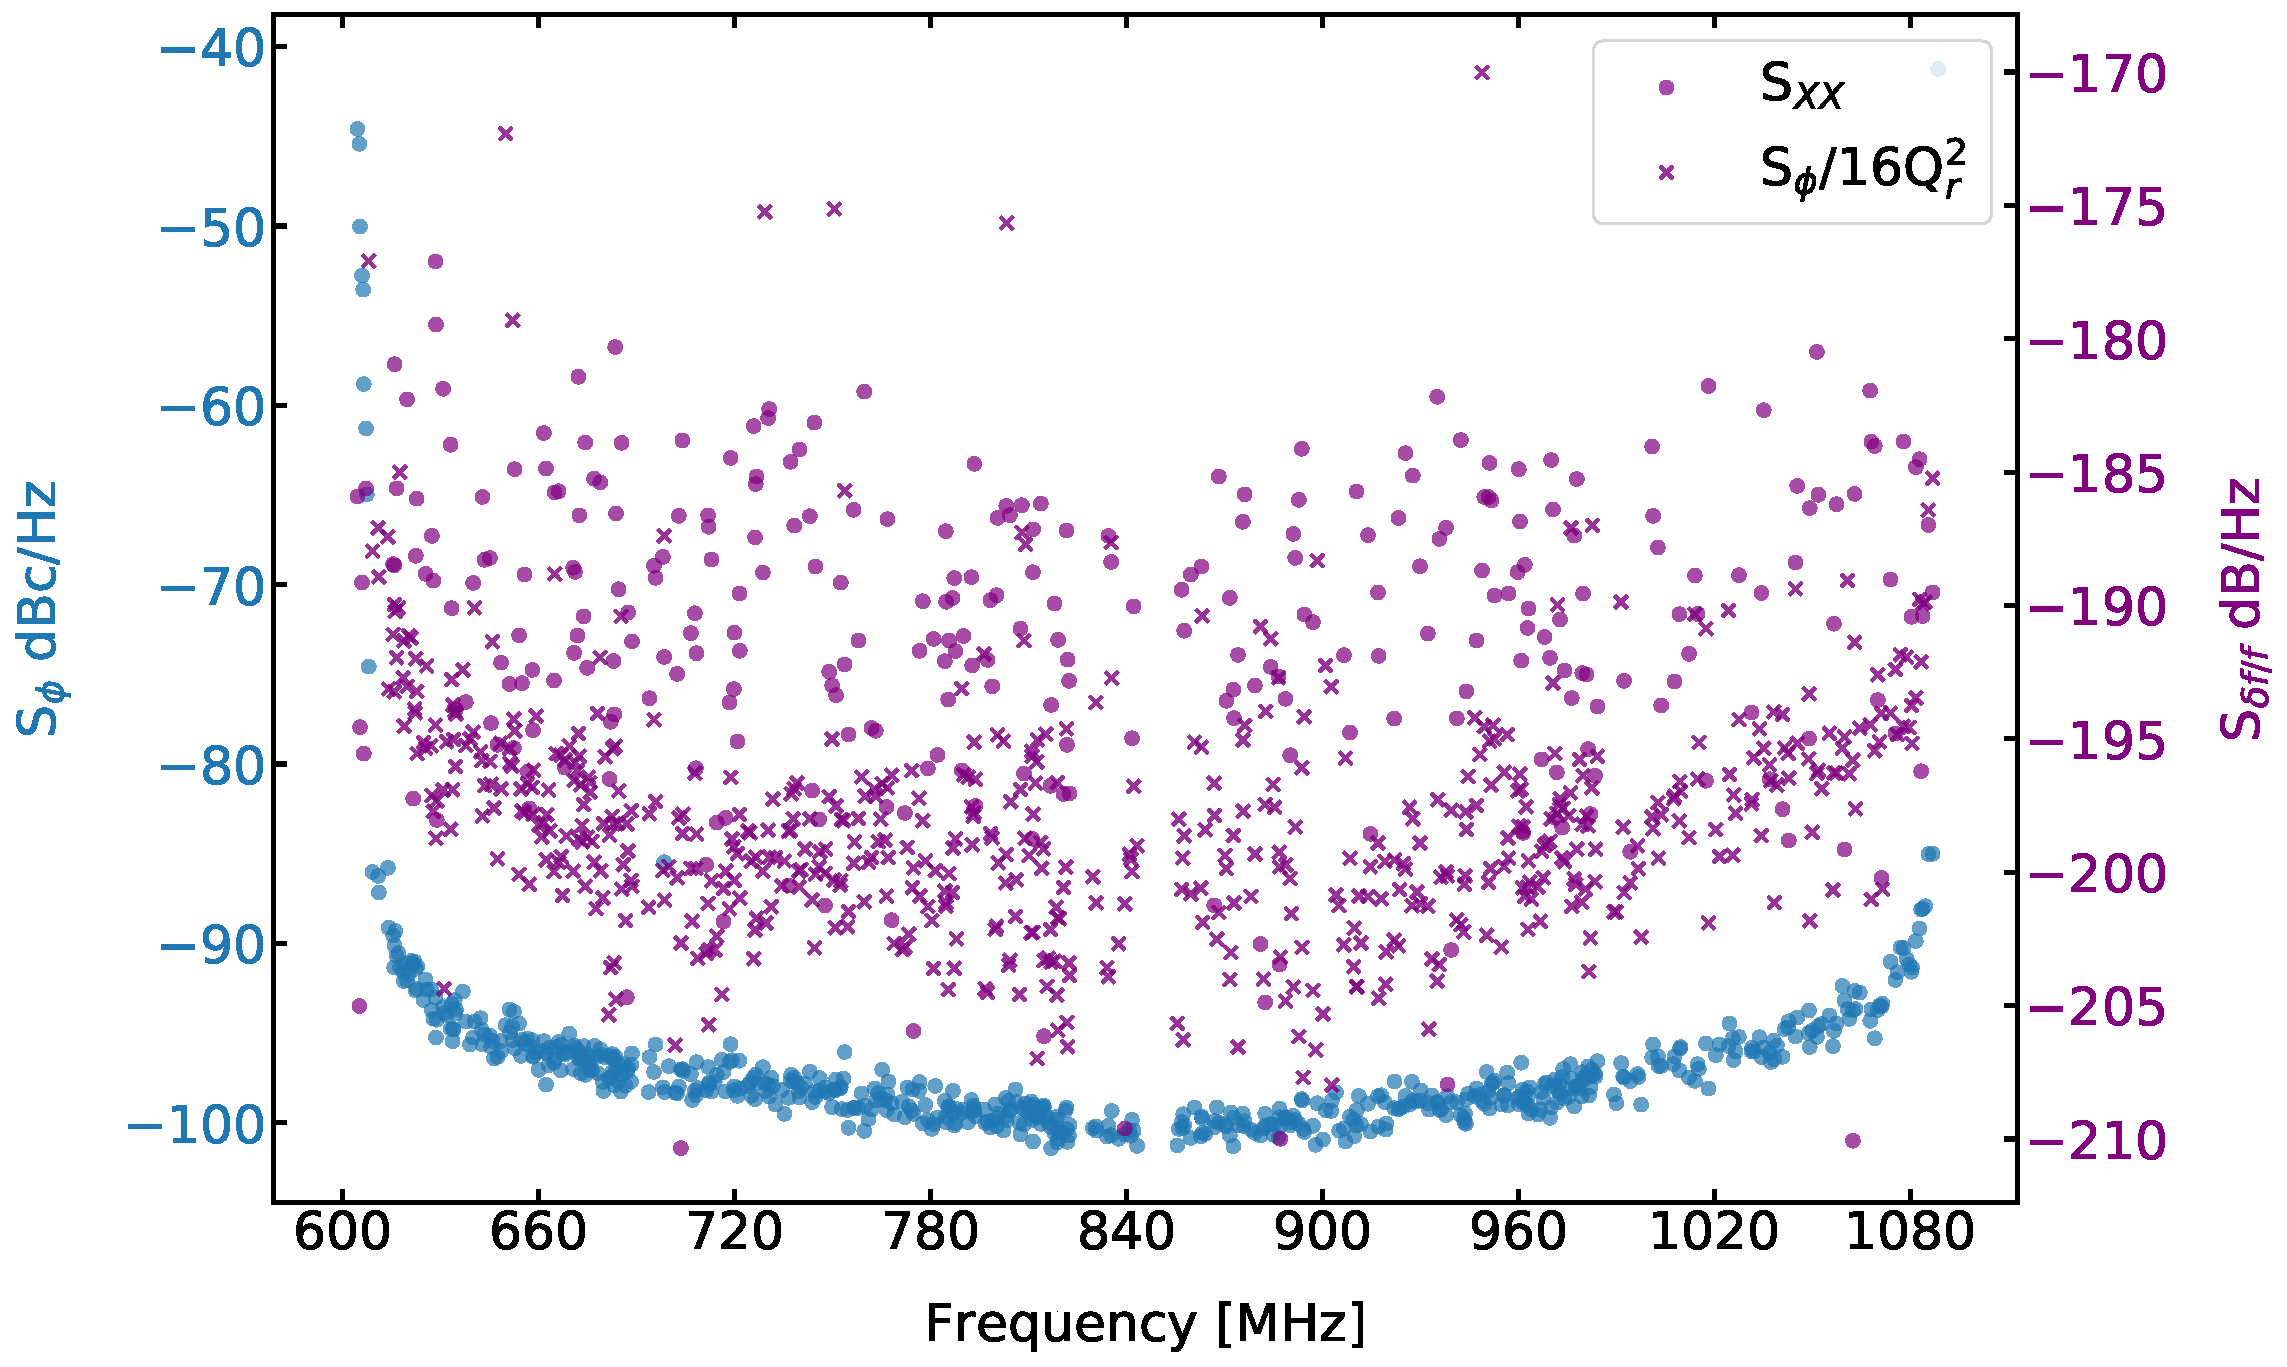
\includegraphics[width=\textwidth]{figures/readout/sim/350_phase_PSDs}
\caption{The white noise in RF loopback mode as a function of probe tone frequency.}
\label{fig:350um PSD comp}
\end{figure}
\end{comment}

\section{Readout Software}\label{software}

A custom software interface is required to operate the ROACH2 firmware and IF electronics, both in a lab setting and during instrument operation. The extent to which the software is automated depends on the context in which the system is being used. For example, if the system is to be used on a balloon platform (e.g., BLAST-TNG, OLIMPO), most if not all of the software functionality should be automated. At a ground/mountain-based observatory (e.g., TolTEC, MUSCAT, SuperSpec), user input on the observer's part should be incorporated when the outcome of a decision can affect the quality of the data (e.g., during the channel selection stage of operation). Basic housekeeping functions, which include uploading the FPGA firmware, initializing software registers such as the DDC delay and writing and programming probe tone combs tones frequency combs, should be automated no matter the context. Other functions, such as the acquisition of diagnostic snap-block data and the setting of RF power levels via the programmable attenuators, should be easily accessible to the operator.

For lab-based system operation, an open-source \texttt{Python}-based software was developed, known as kidPy\footnote{\url{https://github.com/sbg2133/kidPy}}. KidPy is a terminal user interface (TUI) which enables the manual operation of every step which is required to run the readout and acquire data. For the BLAST-TNG flight code (MCP), kidPY was ported to \texttt{C} and fully automated. The BLAST-TNG readout software and in-flight operational strategy is detailed in Appendix~\ref{mcp}.
